\author{Mai L. Ajspur, Rune M. Jensen}
\documentclass[a4paper,twoside,10pt]{article}
\interfootnotelinepenalty=10000
\usepackage[USenglish]{babel} %francais, polish, spanish, ...
\usepackage[T1]{fontenc}
%\usepackage[ansinew]{inputenc}
\usepackage{color}
\usepackage{mathtools}
%\usepackage{hyperref}
\usepackage{subfig}


\usepackage{lmodern} %Type1-font for non-english texts and characters
\usepackage{algorithm}
\usepackage[noend]{algpseudocode}
\usepackage{mnsymbol}

%% Packages for Graphics & Figures %%%%%%%%%%%%%%%%%%%%%%%%%%
\usepackage{graphicx} %%For loading graphic files
\usepackage{amsmath}
\usepackage{amsthm} 
\usepackage{thmtools}
\usepackage{amsfonts}
\usepackage[all,cmtip]{xy}
\usepackage{tikz}

\usepackage{TechFront}
%\declaretheorem{Lemma}
%\declaretheorem{prop}

%\DeclareMathOperator{\sign}{sgn}
%\DeclareMathOperator{\coef}{coef}
%\DeclareMathOperator{\var}{var}
%\DeclareMathOperator{\eqs}{eqs}
%\DeclareMathOperator{\feas}{feas}
%\DeclareMathOperator{\UB}{UB}
%\DeclareMathOperator{\lb}{lb}
%\DeclareMathOperator{\FMcomb}{FM-comb}
%\DeclareMathOperator{\Gcomb}{Gauss-comb}
%\DeclareMathOperator{\proj}{proj}
%\DeclareMathOperator{\Pos}{Pos}
%\DeclareMathOperator{\Neg}{Neg}
%\DeclareMathOperator{\rhs}{rhs}
\newcommand{\sign}{\mathit{sgn}}
\newcommand{\coef}{\mathit{co}}
\newcommand{\var}{\mathit{var}}
\newcommand{\VAR}{\mathit{VAR}}
\newcommand{\eqs}{\mathit{eqs}}
\newcommand{\feas}{\mathit{feas}}
\newcommand{\UB}{\mathit{UB}}
\newcommand{\UBc}{\mathit{UBineq}}
\newcommand{\lb}{\mathit{lb}}
\newcommand{\lbc}{\mathit{lbineq}}
\newcommand{\FMcomb}{\mathit{FM}}
\newcommand{\Gcomb}{\mathit{GA}}
\newcommand{\proj}{\mathit{proj}}
\newcommand{\Pos}{\mathit{Pos}}
\newcommand{\Neg}{\mathit{Neg}}
\newcommand{\rhs}{\mathit{rhs}}
\newcommand{\bounds}{\mathit{bounds}}
\newcommand{\ie}{\mathcal{IE}}
\newcommand{\xx}{\mathcal{X}}
\newcommand{\vea}{\mathbf{co}}
\newcommand{\ttt}{\texttt{t}}
\newcommand{\trt}[1]{\texttt{#1}}
\newcommand{\mi}{\mathit}

\newcommand{\false}{\texttt{false}}
\newcommand{\true}{\texttt{true}}
\newcommand{\nul}{\texttt{null}}
\newcommand{\ve}{\mathbf}
%\newcommand\lhs[1]{\text{lhs}(#1)}
%\newcommand\rhs[1]{\text{rhs}(#1)}
%\newcommand\coef[1]{\text{coef}(#1)}
%\newcommand\LB[1]{\text{LB}_{#1}}
%\newcommand\UB[1]{\text{UB}_{#1}}
\newcommand{\lig}[4]{\ve{#1}\cdot\ve{#2}#3#4}
\newcommand\red[1]{\textcolor{red}{#1}}
\newcommand\blue[1]{\textcolor{blue}{#1}}
\newcommand{\set}[2]{\{\;{#1}\;|\;{#2}\;\}}
\newcommand{\odef}{\overset{\text{def.}}=}
\newcommand{\mc}{\mathcal}
\algdef{SE}[DOWHILE]{Do}{doWhile}{\algorithmicdo}[1]{\algorithmicwhile\ #1}%
\newcommand{\argmin}{\operatornamewithlimits{argmin}}
\newcommand{\StateInd}{\State\hspace{\algorithmicindent}}
\newcommand{\pr}{\mathit{PR}}
\newcommand{\prs}{\mathit{PRS}}
\newcommand{\ens}{\Leftrightarrow}

%\algdef{SE}[DOPAR]{DoPar}{doParWhile}{\algorithmicdo\textbf{ in parallel for\ }}[1]{\algorithmicwhile\ #1}%
\algdef{SE}[DOPAR]{DoPar}{doParUntil}{\algorithmicdo\textbf{ in parallel for\ }}[1]{\algorithmicuntil\ #1}%

\algdef{SE}[SUBALG]{Indent}{EndIndent}{}{\algorithmicend\ }%
\algtext*{Indent}
\algtext*{EndIndent}

\newtheorem{prop}{Proposition}
\newtheorem{lemma}{Lemma}
\newtheorem{cor}{Corollary}

\newcounter{para}
%\newcommand\mypara[1]{\par\refstepcounter{para}\textbf{\thep‌​ara\space#1\space}}
\newcommand\mypara[1]{\newline\par\refstepcounter{para}\textbf{\thepara}\space \textbf{#1} \space}
%\newcommand\mypara{\par\refstepcounter{para}\thepara\space}
%\usepackage[thmmarks,...]{ntheorem}
\newcommand{\Sec}{F}
\newcommand{\Ca}{\mi{Cap}}
\newcommand{\Vol}{\mi{V}}
\newcommand{\Weight}{\mi{W}}
\newcommand{\weight}{\mi{w}}
\newcommand{\BonjeanStations}{\mi{BS}}
\newcommand{\bonjean}{bf}
\newcommand{\Bonj}{B}
\newcommand{\shear}{\mi{sf}}
\newcommand{\Prop}{P}

\theoremstyle{definition}
%\newtheorem{example}{Example}[section]
\newtheorem*{theorem}{Theorem}

\theoremstyle{definition}
\newtheorem{examplex}{Example}[section]
\newenvironment{example}
  {\pushQED{\qed}\renewcommand{\qedsymbol}{$\triangle$}\examplex}
  {\popQED\endexamplex}
	
%\newtheoremstyle{named}{}{}{\itshape}{}{\bfseries}{.}{.5em}{\thmnote{#3}}
%\theoremstyle{named}
%\newtheorem*{namedtheorem}{Theorem}

%\Ttitle{A Fourier-Motzkin-Based Framework to Derive Capacity Models of Container Vessels}%\Ttitle{A Fourier-Motzkin Elimination Framework to Derive Accurate Capacity Models of Container Vessels}
%\Ttitle{Using Decomposed Fourier-Motzkin Elimination to Derive Capacity Models of Mega 
%\title{A Decomposed FME Algorithm to Derive Capacity Models of Mega Container Vessels}
%\title{A Hierarchically Decomposed and Parallelized Fourier-Motzkin-Elimination Algorithm for Massive Variable Elimination Applied to Stowage Optimization Models for Mega Container Vessels}
\Tmonth{January}
\Tyear{2017}

\Ttrnumber{197}      
\TISBNno{978-87-7949-365-0}

\Tauthors{Mai Lise Ajspur\\ Rune M{\o}ller Jensen}
\Ttitle{Using Fourier-Motzkin-Elimination to Derive Capacity Models of Container Vessels}


\begin{document}
\makefront
\maketitle
\begin{abstract}
Due to its high computational complexity, Fourier-Motzkin-Elimination (FME) is mainly known as a theoretical approach to determine feasibility of a linear program (LP). Current practical applications of FME in static program analysis and logic programming exploit that it is a transformation corresponding to existential quantification in logic, but large-scale variable elimination has not been attempted so far. In this report, we introduce a novel FME-based framework for massive variable elimination that takes advantage of the block structure found in many LP problems. Our objective is to simplify the LP by eliminating most of its variables. We show that this is possible for defining accurate capacity models for container vessels by deriving them from stowage models. 
\end{abstract}

%\tableofcontents

\section{Introduction}

Fourier-Motzkin-Elimination (FME) is a central theoretical approach to determine feasibility of linear programs (LPs), but it is seldom used in practice due to its high computational complexity.
%
It is an algorithm that projects the polyhedron of feasible solutions of the LP one dimension at a time, such that the feasible values and inter-dependencies of the remaining variables in the resulting polyhedron are unaltered. In this way, FME computes an abstraction of the original LP corresponding to existential quantification in logic, \red{where the value of the eliminated variable no longer is represented.}

Projection is a fundamental operation that has been successfully applied in practice, in particular in static analysis of programs and logic programming,
%, and constraint logic programming (e.g., \cite{fouilhe,benoy05,simon10,jaffar93}), 
(see e.g. \cite{benoy05} for applications and references). Here polyhedra represent 
numerical variable domains \cite{cousot78}, and variables out of scope and other auxiliary variables are eliminated via projection. Likewise, projection is used in constraint query languages \cite{lassez90}, and other potential applications of FME include %constraint query languages \cite{lassez90}, 
coordination and/or negotiation situations as suggested in \cite{lukatskii08}, and as an alternative solution method for parametric linear programming \cite{jones08}.

We are not aware of any previous work, however, that applies FME for massive variable elimination, where say 99\% of the variables are eliminated with the purpose to simplify the LP by removing most of its variables.This is, however, a relevant task. Consider for instance an economic model that achieves high accuracy through a large number of economic parameters at county level, but primarily is used to analyse these parameters at an aggregated national level. In this case, only a small fraction of the variables are of interest and the LP may be simplified by abstracting away (i.e., eliminating) the other low-level variables.

In this report, we consider a similar problem. In liner shipping, it is challenging to evaluate how the cargo capacity of a container vessel depends on the {\em cargomix}, i.e., the mixture of containers with different attributes that the vessel carries. The reason for this is that containers only can be stowed certain ways (e.g., $40'$ containers cannot be stowed on top of $20'$ containers and refrigerated containers must be stowed in slots with power plugs) while at the same time the vessel must fulfill seaworthiness requirements such as stability rules and stress force limits. The liner shipping companies need accurate capacity models to optimize decisions about cargo flow and uptake management on services, but today they rely on static capacity measures (e.g., \cite{ting04,feng08,zurheide13}) that are too inaccurate for practical usage \cite{AlbertosThesis}.

On the other hand, accurate LP models for optimization of vessel stowage planning have been developed (e.g., {\cite{pacino11,pacino12,AlbertosThesis}}). These models represent a feasible stowage plan as the number of containers of different type and weight class that the vessel can carry in each of its $100$ or more storage areas. A capacity model is simply an abstraction of these stowage models, where the physical position of cargo is abstracted away. Since there are in the order of $100$ storage areas on the vessel, this corresponds to eliminating $99\%$ of the variables. 

In this report, we introduce a novel hierarchically decomposed and parallelized FME algorithm for massive variable elimination. Similar to other recent FME frameworks (e.g., \cite{simon05,lukatskii08,shapot12}), our method applies Gauss\--eli\-mi\-na\-tion (equality removal), removal of syntactic and quasi-syntactic redundancies, complete removal of redundancy in between variable eliminations, together with an approximation of the projection when needed. In addition, our framework includes preprocessing including removal of less strict inequalities. 
Our main contribution, however, is a hierarchical decomposition of the problem using auxiliary variables based on the block structure that often is observed in LPs \cite{williams} as well as a sound, concurrent implementation of the redundancy removal. 

Theoretically, the number of inequalities may grow double exponentially with the number of eliminated variables. Our experiments on deriving capacity models from stowage models of mega vessels, however, show only a modest growth in the number of inequalities  when complete removal of redundant inequalities between each variable elimination is carried out (e.g., see Figures~\ref{fig:FinalProjectionS1}-\ref{fig:FinalProjectionS3} in Chapter~\ref{sec:results}). As expected, the number of inequalities decrease in the end where most variables are removed. The resulting capacity models are small and useful in practice (e.g., see Table~\ref{tab:results} in Chapter~\ref{sec:results}). 

It is possible that the limited growth in non-redundant inequalities is unique for deriving capacity models, but since we mainly exploit the block structure of stowage models, we believe that similar results can be obtained in other domains.
\\
\\
The remainder of this report is organized as follows.
In Chapter~\ref{sec:def}, we present the definitions and notation relating to inequality systems and projections that are used in this report. 
Chapter~\ref{sec:basic} outlines the basic algorithms used for achieving the projection, namely the classical Fourier-Motzkin elimination, Gauss-elimination, and some basic methods for preprocessing and removing redundant information (inequalities). 
In Chapter~\ref{sec:improvements} we then describe the alterations and improvements made to these algorithms. Specifically we detail an altered and parallellized method for removing redundancy, how we combine the mentioned steps into an algorithm for projection, and we present how our system (as well as other block structured systems) can be decomposed to achieve a more efficient projection.    
Subsequently, Chapter~\ref{sec:results} gives a short presentation of the considered stowage model(s) after which the results of projecting these are presented along with a few details regarding the implementation. 
Finally, we review and discuss related work in Chapter~\ref{sec:related} before Chapter~\ref{sec:conclusion} concludes.

\section{Definitions and notation}\label{sec:def}
In this report we consider a finite set of variables $\xx$ plus the set $\ie$ consisting of all inequalities and equalities over any subset of $\xx$. An element $c\in\ie$ is thus an equality or inequality over a subset $\VAR(c)\subseteq\xx$ and is referred to as an (in)equality over $\VAR(c)$. 
It can be written as
\begin{equation}\label{eq:ineq}
c: \sum_{x\in \VAR(c)}\coef(x,c)\cdot x\odot_c \rhs(c),
\end{equation} 
where $\odot_c\in\{=, \leq\}$ is the \emph{relation} of $c$, $\coef(x,c)\in\mathbb{R}$ is the \emph{coefficient} of $x$ in $c$ for any $x\in \VAR(c)$, and $\rhs(c)\in\mathbb{R}$ is the \emph{right-hand-side} of $c$.
%
Letting $\coef(x,c)= 0$ for all $x\in \xx\setminus\VAR(c)$, we can extend $c$ to $X$ for any set $X\subseteq \xx$ by letting $c_X$ be the (in)equality over $X$ given by
\begin{equation}\label{eq:constraintX}
c_{X}: \sum_{x\in X} \coef(x,c)\cdot x \odot_c\rhs(c).
\end{equation}
Assuming a given total order $\preceq$ on the variables in $\xx$ we can order and name the variable of any subset $X\subseteq \xx$ according to this order such that $X = \{x_1, x_2, \ldots, x_{|X|}\}$ and $x_1\prec x_2\prec \ldots \prec x_{|X|}$. 
Letting $\vea(c_X) \odef (\coef(x_1,c),\ldots,$ $\coef(x_{|X|},c))$ and $\ve{x}_X = (x_1,\ldots, x_{|X|})$, the constraint $c_X$ can also be written using the dot-product as $c_X:\vea(c_X)\cdot\ve{x}_X\odot_c \rhs(c)$. 
By definition $c_{\VAR(c)}$ equals $c$, so we let $\vea(c)\odef \vea(c_{\VAR(c)})$, and for convenience we leave out the subscript of $\ve{x}_X$ when the $X$ is implied e.g. by the coefficient vector in the dot product. 

We let $\var(c)$ denote the variables whose coefficient in $c$ is nonzero, i.e. $\var(c)\odef \set{x\in \VAR(c)}{\coef(x,c) \neq 0}$ $\subseteq \VAR(c)$, and we notice that we might have that $\var(c)\subset \VAR(c)$. When $VAR(c)$ is clear from context we allow ourselves to write $c$ as $c : \sum_{x\in \var(c)}\coef(x,c)\cdot x \odot_c \rhs(c)$.

The set of points in $\mathbb{R}^{|\VAR(c)|}$ that satisfies the (in)equality $c$ is called the \emph{feasible region} for $c$ and is hence defined as
\[
\feas(c) \odef \set{\ve{r}\in\mathbb{R}^{|\VAR(c)|}}{\vea(c)\cdot\ve{r}\odot_c \rhs(c)}.
\] 
Since the feasible region of an (in)equality is just a set of points in a (multi-dimensional) Euclidian space, here the order of the variables, $\prec$, is important and needs to be explicitly or implicitly given or assumed.
\\\\
In the following, an (in)equality system is a set $S$ of (in)equalities over the same set of variables, $\VAR(S)$, i.e. $S\subset\ie$ and $\VAR(c)=\VAR(S)$ for all $c\in S$. Therefore, when we union, intersect or subtract two (in)equality systems $S_1, S_2\subset \ie$ to produce another (in)equality system $S'$, it is required that all (in)equalities in $S'$ are (in)equalities over the same set $X$. Hence we require that $\VAR(S_1) = \VAR(S_2)$ when we talk about the (in)equality systems $S_1\cup S_2$, $S_1\cap S_2$ or $S_1\setminus S_2$. However, it is always possible to extend the (in)equalities in $S_1$ and $S_2$ to a common variable-set, and if $\VAR(S_1)\neq \VAR(S_2)$ we therefore let $S_1\cup S_2\odef \set{c_X}{c\in S_1}\cup \set{c_X}{c\in S_2}$, where $X=\VAR(S_1)\cup\VAR(S_2)$, and similar for the other set-operations $\cap$ and $\setminus$. 

We let $\eqs(S)$ denote the set of equalities in $S$, i.e. $\eqs(S) \odef \set{c \in S}{\odot_c \text{ is } =}$, we define the used variables in $S$ as
$\var(S)\odef \cup_{c\in S}\var(c)$, and we let $S_X \odef \set{c_X}{c\in S}$ for any $X\subseteq \xx$.
The feasible region for $S$ is the set of points in $\mathbb{R}^{|\VAR(S)|}$ that satisfies \emph{all} (in)equalities in $S$, i.e. 
\[
\feas(S) \odef \cap_{c\in S}\feas(c).
\]
It follows that if $S_1, S_2\subseteq S$, then $\feas(S_1\cup S_2) = \feas(S_1)\cap \feas(S_2)$. 

In linear programming, it is common to have bounds for some of the variables in an (in)equality system $S$. For our purpose, upper and lower bounds are modeled as inequalities as in \eqref{eq:constraintX} with $X=\VAR(S)$ and a coefficient of $\pm 1$. If they exist, the inequalities representing upper and lower bounds for $x$ are referred to as $\UBc(x)$ and $\lbc(x)$, respectively, while $\UB(x)\in \mathbb{R}$ and $\lb(x)\in\mathbb{R}$ denote the upper, respectively lower bound of the variable $x$. 
That is, if the upper bound of $x$ exists, then $\UBc(x)$ refers to the inequality $x\leq \UB(x)$ in $S$, and if the lower bound of $x$ exists, then $\lbc(x)$ refers to the inequality $-x \leq -\lb(x)$ in $S$.

{We say that two (in)equality systems $S_1$ and $S_2$ are \emph{equivalent} and write $S_1\cong S_2$ if 
$\VAR(S_1)=\VAR(S_2)$ and $\feas(S_1) = \feas(S_2)$.}

An (in)equality $c\in S$ is \emph{redundant} if $c$ does not influence the feasible region for $S$, i.e. if $\feas(S)=\feas(S\setminus\{c\})$. The redundancy of an \emph{in}equality $c: \vea(c)\cdot\ve{x}\leq \rhs(c)$ can be determined by maximizing its left-hand-side:  
\begin{equation}\label{eq:redundant}
c \text{ is redundant iff }\max\set{\vea(c)\cdot\ve{r}}{\ve{r}\in \feas(S\setminus\{c\})} \leq \rhs(c).
\end{equation}
The equality $c: \vea(c)\cdot\ve{x} = \rhs(c)$ 
is redundant iff both inequalities 
$\vea(c)\cdot\ve{x} \leq \rhs(c)$ and $-\vea(c)\cdot\ve{x} \leq -\rhs(c)$ 
are redundant.
If the (in)equality $c$ is \emph{not} redundant, it is called \emph{non-redundant}.
%
\\\\
As described, the feasible region of $S$ describes the combination of values for the variables in $\VAR(S)$ that satisfy all the (in)equalities in $S$. However, for the sake of abstraction there are some variables $Y\subseteq \VAR(S)$ whose value we are not interested in, we just want to know that a satisfying value for these variables exists.  
Therefore, we want to find a set of values $P$ for the variables of interest ($\VAR(S)\setminus Y$), such that when we have a set of values in $P$ then we can extend it with values for the variables in $Y$ in such a way that the collective set of values satisfy all (in)equalities in $S$. 
The {projection} of the feasible region of $S$ gives us the largest set of values with this property.

Let $S$ be an (in)equality system over $X$ and let $Y\subseteq X$ be the set of variables that we want to eliminate. Without loss of generality we can assume that $X = \{x_1,\ldots, x_{|X|}\}$, $x_1\prec \ldots \prec x_{|X|}$ and that $Y=\{x_i, x_{i+1}, \ldots, x_{|X|}\}$ for some $1\leq i\leq |X|$.
The {projection} of the polyhedron $\feas(S)$ with respect to $Y$ is then the polyhedron 
\[
\proj_Y\big(\feas(S)\big) \odef \set{\ve{r}\in\mathbb{R}^{|X\setminus Y|}}{\text{there exists an } \ve{r}'\in\mathbb{R}^{|Y|}\text{ such that }
(\ve{r},\ve{r'})\in \feas(S)}.
\]
See Figure~\ref{fig:proj}. Here $(\ve{r},\ve{r'})$ denotes the vector $(r_1,\ldots, r_{|X\setminus Y|}, r'_1,\ldots, r_{|Y|})$ where $\ve{r}=(r_1,\ldots, r_{|X\setminus Y|})$ and $\ve{r'}=(r'_1,\ldots, r_{|Y|})$.

For convenience of notation we let $\proj_{Y'}\big(\feas(S)\big) = \proj_{Y'\cap \VAR(S)}(\feas(S))$ for any $Y'\subseteq \xx$.

\begin{figure}
	\centering
		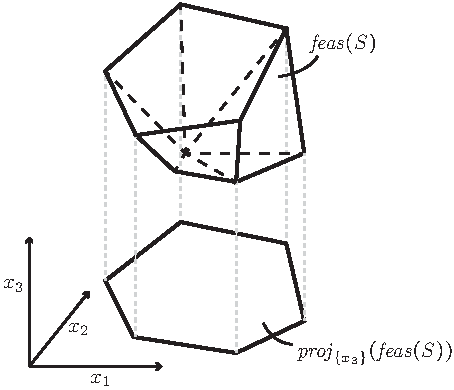
\includegraphics{figures/projection.pdf}
	\caption{Projection of the polyhedron $\feas(S)$ in $\mathbb{R}^3$ with respect to the third variable }
	\label{fig:proj}
\end{figure}
We notice that for arbitrary subsets $Y_1$ and $Y_2$ of $Y$ such that $Y_1\dot\cup Y_2=Y$,\footnote{$\dot\cup$ denotes disjoint union.} we have that $\proj_Y(P)=\proj_{Y_1}(\proj_{Y_2}(P))$. 
\\\\
In this report, we will only be interested in the projection of the feasible region of (in)equality systems,
and these are the feasible sets of (other) (in)equality systems (see e.g. \cite{ziegler95}). What we are interested in are the dependencies among the non-projected variables,  
so we want to talk about a system that ``generates'' a certain projection. For this we define $\prs_Y(S)$ to be the set of (in)equality systems whose feasible set is the projection of $S$ w.r.t. $Y$, i.e. 
\[
\prs_Y(S)\odef \set{S'\subset\ie}{\VAR(S')=\VAR(S)\setminus Y \text{ and }\feas(S') = \proj_Y\big(\feas(S)\big)}.
\]
If $S'\in\prs_Y(S)$ we say that $S'$ is a \emph{projection of $S$ w.r.t. $Y$}.
 
We point out, that for arbitrary (in)equality systems $S_1,S_2\subset \ie$ and $Y_1,Y_2\subseteq \xx$, the sets $\proj_{Y_1}(\feas(S_1))$ and $\proj_{Y_2}(\feas(S_2))$ are just sets of points in $\mathbb{R}^{|\VAR(S_1)\setminus Y|}$ and $\mathbb{R}^{|\VAR(S_2)\setminus Y|}$, respectively. As long as $|\VAR(S_1)|=|\VAR(S_2)|$ these sets can therefore be intersected, unioned or subtracted, but in order to have a meaningful interpretation of 
e.g. $\proj_{Y_1}(\feas(S_1))\cap\proj_{Y_2}(\feas(S_2))$ in our setting, we must have that $\VAR(S_1)\setminus Y_1 = \VAR(S_2)\setminus Y_2$, and projections must be given according to the same, implicitly given order $\prec$ on $\xx$.
%
\\\\
For proving the correctness of our decomposition in Section~\ref{sec:decomp} we need the following minor propositions.
\begin{restatable}{lemma}{projection}\label{lm:projection}
Let $S, S_1, S_2\subset\ie$ be (in)equality systems over $X$ and let $Y\subseteq X$. 
\begin{enumerate}
\item\label{lm:1.1} Assume that $\var(S_1)\cap\var(S_2) = \emptyset$. Then 
\begin{equation}\label{eq:lm1.1}
\proj_Y\big(\feas(S_1\cup S_2)\big) = \proj_Y\big(\feas(S_1)\big)\cap \proj_Y\big(\feas(S_2)\big).
\end{equation}
\item\label{lm:1.2} Assume that $\var(S_1)\cap Y = \emptyset$. Then
\begin{equation}
\proj_Y\big(\feas(S_1\cup S_2)\big) = \feas\big((S_1)_{X\setminus Y}\big)\cap \proj_Y\big(\feas(S_2)\big).
\end{equation}
\item\label{lm:1.3} Let $X'\subseteq \xx$ be a super set of $X$, i.e. $X\subseteq X'$, and let $E$ be an (in)equality system such that $\proj_Y\big(\feas(S)\big) = \feas(E)$.
Then 
\[
\proj_Y(\feas(S_{X'})) = \feas(E_{X'\setminus Y}).
\]
\end{enumerate}
\end{restatable}
\begin{proof} See Appendix.
\end{proof}
\section{Basic Algorithm}\label{sec:basic}
\subsection{Fourier-Motzkin-elimination}
Traditionally, this method works on pure inequality systems (i.e. with no equalities), and we will describe it like that. Since, an (in)equality system easily can be translated into a pure inequality system, this does not cause any problems. The method is described below.

The method eliminates the variables in $Y\subseteq X$ by creating new inequality systems in a stepwise fashion. At each step, one of the variables in $Y$ is eliminated from the current system to obtain the next system. A variable $x\in Y$ is projected from the pure inequality system $S$ as follows (see e.g. \cite{imbert93} or \cite{ziegler95}).

Firstly, the inequalities are divided into disjoint sets depending on the sign of the variable's coefficient in the constraints. Thus, we define
\begin{eqnarray*}
\Pos_S(x) &\odef& \set{c\in S}{\coef(x,c) > 0},\\
\Neg_S(x) &\odef& \set{c\in S}{\coef(x,c) < 0}, \text{ and }\\ 
\mathit{Zero}_S(x) &\odef& \set{c\in S}{\coef(x,c) = 0}.
\end{eqnarray*}
To eliminate the variable $x$ and construct the next inequality system, we first set aside $\mathit{Zero}_S(x)$, or rather $\set{c_{X\setminus\{x\}}}{c\in \mathit{Zero}_S(x)}$. To this set we then add a new inequality for each combination of $c^+\in\Pos_S(x)$ and $c^-\in\Neg_S(x)$. This new inequality is constructed by first normalizing $c^+$ and $c^-$ such that their coefficients for $x$ are plus and minus $1$, respectively, and then the two normalized inequalities are added. In this inequality, the coefficient of $x$ is zero, and restricting the inequality to $X\setminus\{x\}$ we then get
%is the inequality $\ve{a}\cdot \ve{x}\leq b$ and $c^-$ is the inequality $\ve{a}'\cdot \ve{x}\leq b'$, the resulting 
the inequality $\FMcomb(x,c^+, c^-)$ over $X\setminus\{x\}$ given below. %-comb$c^+ \boxplus_x c^-$, 
\begin{multline}
%\begin{split}
\label{eq:FMcomb}
%\MoveEqLeft
\FMcomb(x,c^+, c^-):\\ 
\sum_{x'\in \VAR(S)\setminus\{x\}} \left(\frac{1}{\coef(x,c^+)}\coef(x',c^+) + \frac{1}{\coef(x,c^-)}\coef(x',c^-)\right)\cdot x'
\leq \frac{1}{\coef(x,c^+)}\rhs(c^+) + \frac{1}{\coef(x,c^-)}\rhs(c^-)
% 
%\left(\frac{1}{\coef(x,c^+)} \ve{a} +\frac{1}{-\coef(x,c^-)} \ve{a}'\right)\cdot\ve{x} \leq \frac{1}{\coef(x,c^+)}b +\frac{1}{-\coef(x,c^-)}b'.
%\end{split}
\end{multline}
%This inequality clearly does not use $x$ (the coefficient is $0$).%
%
The procedure is described in pseudocode in Algorithm~\ref{alg:FMBasic}.

When eliminating a variable $x_i$, the inequalities in the constructed set $S'$ are all implied by the inequalities in $S$. On the other hand, it also holds that if $(x_1, x_2, \ldots, x_{i-1}, x_{i+1}, \ldots, x_n)$ satisfies the inequalities in $S'$ then there exists an assignment to $x_i$ such that $(x_1, x_2, \ldots, x_{i-1}, x_i, x_{i+1}, \ldots, x_n)$ satisfies the inequalities in $S$ {(e.g. \cite{duffin74}, Lemma 1)}. That is, $S' = \proj_{\{x_i\}}(S)$.
%\marginpar{How to write it without using the index $i$?}

A disadvantage of the procedure is its complexity. Due to the combination of inequalities in each step, in the worst case scenario where $|\Pos_S(x)| = |\Neg_S(x)| = \frac{|S|}{2}$ for the current system $S$, the number of inequalities in the succeeding system is $\frac{1}{4}|S|^2$. This implies that (both time and space) complexity is double-exponential.  
We also notice that the denser the system is, the more it will grow. 
It should, however, also be emphasized that not all inequalities in a succeeding system are necessarily non-redundant. In fact, the
number of non-redundant inequalities can only grow in single exponential \cite{Monniaux10}.
%
\begin{algorithm}
\caption{Eliminating variables from an inequality system $S$ using Fourier-Motzkin-elimination.}\label{alg:FMBasic}
\begin{algorithmic}[1]
\Function{FM-Elim}{Inequality system $S$, variables to eliminate $Y\subseteq \VAR(S)$}
	\State  $S'\gets S$, $Y'\gets Y$
	\While{ $Y'\neq \emptyset$ }
		\State $x\gets$ \Call{ChooseVariableToDelete}{$Y'$, $S'$}
		\State $S' \gets$ \Call{FM-ElimVar}{$S'$, $x$}
		\State Remove $x$ from $Y'$
	\EndWhile
	\State \Return $S'$
\EndFunction
\Statex
\Function{FM-ElimVar}{Inequality system $S$, variable to eliminate $x\in var(S)$}
\State Divide $S$ into $\Pos_S(x)$, $\Neg_S(x)$ and $\mathit{Zero}_S(x)$
\State $S'\gets \set{c_{\VAR(S)\setminus\{x\}}}{c\in\mathit{Zero}_S(x)}$ 
\ForAll{$c^+ \in \Pos_S(x)$}
	\ForAll{$c^- \in \Neg_S(x)$}
		\State Add $\FMcomb(x,c^+, c^-)$ to $S'$\Comment see \eqref{eq:FMcomb}
	\EndFor
\EndFor
\State \Return $S'$
\EndFunction
\end{algorithmic}
\end{algorithm}
%
The function \Call{ChooseVariableToDelete}{} in Algorithm~\ref{alg:FMBasic} is a heuristic to determine which variable among the ones needed to be eliminated that should be eliminated first. In principle, there are many choices for heuristics, but the most commonly used heuristic is the greedy heuristic that aims at minimizing the size of the inequality system in the next step \cite{duffin74}\footnote{This heuristic was useful for us, but though it is very commonly used, note that its success may depend on the specific problems considered; Imbert \cite{imbert93} states in his conclusion to have found the related heuristic returning $\argmin_{y\in Y}|\Pos_S(y)||\Neg_S(y)|$ to be inferior to ``any other choice, even at random''.}. This is easy to calculate from the current system since the increase in size only depends on the size of the sets $\Pos_S$ and $\Neg_S$ for the variable in question. We have also chosen this heuristic, that is, the function \Call{ChooseVariableToDelete}{$Y,S$} returns 
\[
\argmin_{y\in Y}\big(|\Pos_S(y)||\Neg_S(y)| - |\Pos_S(y)|-|\Neg_S(y)|\big).
\] 
%
%
%{It should be noted, though, that Imbert \cite{imbert93} states in his conclusion to have found the related heuristic returning $\argmin_{y\in Y}|\Pos_S(y)||\Neg_S(y)|$ to be inferior to ``any other choice, even at random''. The particular experiments, results and the specific problems considered for the experiments is, however, not presented.}
%
\subsection{Gauss-elimination}
When our (in)equality system contains equalities, it is often an advantage to let them remain equalities instead of converting each one to two inequalities. Firstly, they are then easier to identify, and instead of doing FM-elimination on a variable in an equality, we can isolate it in the equality and substitute it in the other (in)equalities. By doing this, we avoid the increase in inequalities that an FM-elimination of the variable would otherwise (in most cases) cause. The downside is, that we make the system more dense, which FM-elimination, however, does as well. This is e.g. done in \cite{simon05}.

Given an equality $c$, %: \ve{a}\cdot\ve{x} = b$, 
isolating and substituting the variable $x\in \var(c)$ in the (in)equality $c'$ for which $x\in\var(c')$ %: \ve{a}'\cdot\ve{x} \odot_{c'} b'$ 
corresponds to scaling $c'$ and $c$ with $\frac{1}{|\coef(x,c')|}$ and $\frac{-\sign(x,c')}{\coef(x,c)}$, respectively\footnote{$\sign$ is the sign-function that returns $+1$, $-1$ or $0$ depending on the sign of its parameter.}, such that the two coefficients for $x$ are plus and minus 1, and then adding the resulting (in)equalities. Restricting the resulting (in)equality to $\VAR(S)\setminus\{x\}$ results in the inequality $\Gcomb(x,c,c')$ over $\VAR(S)\setminus\{x\}$ given below. %$(-\sign(\coef(x,c'))\boxtimes c)\boxplus_x c'$:
\begin{multline}
%\begin{split}
\label{eq:Gauss}
\Gcomb(x,c,c'):
\sum_{x'\in\VAR(S)\setminus\{x\}}
\left(  \frac{-\sign(\coef(x, c'))}{\coef(x,c)}\coef(x',c) 
+ \frac{1}{|\coef(x, c')|}\coef(x',c')\right)\cdot x' \\
\odot_{c'} \frac{-\sign(\coef(x, c'))}{\coef(x,c)}\rhs(c)+ \frac{1}{|\coef(x,c')|}\rhs(c').
%\left(\frac{-\sign(\coef(x, c'))}{\coef(x,c)}\ve{a}+ \frac{1}{|\coef(x, c')|}\ve{a}'\right)\cdot\ve{x} \odot_{c'} \frac{-\sign(\coef(x, c'))}{\coef(x,c)}b+ \frac{1}{|\coef(x,c')|}b'.
%\end{split}
\end{multline} 
%
In our method, we will define auxiliary variables (that should not be eliminated) and we will therefore have a number of equalities which we will use to make Gauss-elimination. The pseudocode for this step is given in Algorithm~\ref{alg:Gauss}.
%
\begin{algorithm}
\caption{Eliminating variables from an (in)equality system $S$ using Gauss-elimination.}\label{alg:Gauss}
\begin{algorithmic}[1]
\Function{Gauss-Elim}{(In)equality system $S$, variables to be eliminated $Y\subseteq \VAR(S)$}
\State $S'\gets S$
\While{$Y\cap \var(\eqs(S')) \neq \emptyset$}
	\State $(x, c) \gets \Call{ChooseVarInEquality}{Y,S'}$ 
	\State $S'\gets \Call{Gauss-ElimVar}{S', c, x}$
\EndWhile
\State\Return $S'$
\Statex
\Function{Gauss-ElimVar}{System $S$, equality $c$, variable $x\in \var(c)$}
	\State $S'\gets \emptyset$
	\State Remove $c$ from $S$
	\ForAll{$c'$ in $S$}
		\If{$\coef(x, c') = 0$}
			\State Add $c'_{\VAR(S)\setminus\{x\}}$ to $S'$
		\Else
			\State Add $\Gcomb(x,c,c')$ to $S'$ \Comment see \eqref{eq:Gauss}
		\EndIf
	\EndFor
	\State \Return $S'$ 
\EndFunction
\EndFunction
\end{algorithmic}
\end{algorithm}
Also for this procedure, a heuristic is used for choosing which variable - and in this case also which equality - should be used in the elimination. Again, there are many choices and we have decided to %mainly use the one that finds the shortest equation that has a variable in $Y$, and then choose the variable that has the fewest occurrences in the system, or the other way around, 
first find the variable (occurring in equations) that occurs the fewest times, and then find the shortest equation using this variable. I.e. the function \Call{ChooseVarInEquality}{$Y,S$} returns $(y,e)$ where
%\[
%e = \argmin_{c\in \eqs(S)}|\var(c)|\; \text{ and }\;y = \argmin_{x\in \var(e)}|\set{c\in S}{x\in \var(c)}|,
%\] 
%or
\[
y = \smashoperator[r]{\argmin_{x\in \var(\eqs(S))}}|\set{c\in S}{x\in \var(c)}|\; \text{ and }\; e = \smashoperator[r]{\argmin_{c\in \eqs(S).y\in \var(c)}}|\var(c)|.
\] 

\subsection{Preprocessing}
The purpose of preprocessing is to simplify the (in)equality system that we are dealing with, i.e. to reduce it by removing redundant inequalities that are easily identifiable, updating bounds for variables and substituting variables with implied values \emph{such that} $\feas(S)$ does not change. {Likewise, preprocessing can be used to figure out at an early stage whether the problem is infeasible. However, we assume that the problem is feasible and do not spend time on checking this during the preprocessing step.}

Our preprocessing part consists of the following steps, described below: removing empty (in)equalities and unused variables, updating bounds for (in)\-equali\-ties with only one variable, substituting variables with fixed values, eliminating variables with only one sign occurring, updating bounds due to extreme values, removing linearly dependent (in)equalities \cite{lassez93}, and removing less strict (in)equalities. The basic preprocessing steps can be found in e.g. \cite{brearley75}, \cite{andersen95} and \cite{maros}.

When doing these steps, we take into consideration that not all variables should be eliminated, in fact there are some that we need to keep. This is particularly the case when we use auxiliary variables for decomposing our system (see Section~\ref{sec:decomp} later). Therefore we do not remove variables that are not in $Y$, and we do not substitute them with a value during the preprocessing {without keeping track of these substitutions}. 
%
\subsubsection{Removing empty (in)equalities and unused variables}\label{para:emptyIneqs} 
We remove from $S$ all inequalities $c$ for which $|\var(c)| = 0$. %\red{If $\rhs(c)< 0$, or $c$ is an equality and $\rhs(c)\neq 0$, then $S$ is unsatisfiable/infeasible.} 

For all $x\in Y$ for which $x \notin \var(S)$, we simply remove $x$ from $\VAR(S)$, i.e. we restrict $S$ to $\VAR(S)\setminus\{x\}$. Notice that we do not remove variables that we have not specifically expressed a desire to eliminate.
%	
\subsubsection{Updating bounds for (in)equalities with only one variable}\label{para:singleton} For all inequalities $c$ for which $|\var(c)|=1$, we have that $c$ equals the inequality  $\coef(x,c)\cdot x \odot_c \rhs(c)$ for an $x\in X$. In this case, we update the bound(s) for $x$ accordingly. That is, if $\coef(x,c)>0$ and $\frac{\rhs(c)}{\coef(x,c)}<\UB(x)$, then $c$ is removed from $S$ and $\UBc(x)$ is replaced with the inequality $x \leq \frac{\rhs(c)}{\coef(x,c)}$.  
Similarly, if $\coef(x,c)<0$ and $\frac{\rhs(c)}{\coef(x,c)}> \lb(x)$, then $c$ is removed from $S$ and $\lbc(x)$ is replaced with the inequality $-x \leq - \frac{\rhs(c)}{\coef(x,c)}$. 

If $c$ is an equality, both bounds are updated. 
%
\subsubsection{Substituting variables with fixed value}\label{para:fixed} If $\UB(x) = \lb(x)$ for a variable $x\in X$, then we substitute $x$ with the given value in all (in)equalities in $S$. 

If the variable $x$ is not in $Y$, meaning that we have not specified that it should be removed, then we do maintain the bounds of $x$ in the system, i.e. we substitute $x$ in all (in)equalities in $S$ except for $\lbc(x)$ and $\UBc(x)$. The main reason for keeping such inequalities is that due to our decomposition of the system (see Section~\ref{sec:decomp} later) the system might later be joined with another system where $x$ is present and hence $x$'s value should not ``disappear''. 
%\red{If $\lb(x)>\UB(x)$ then $S$ is unsatisfiable/infeasible.}
%
\subsubsection{Eliminating variables with only one sign occurring}\label{para:oneSign} If a variable $x$ only occurs with a non-negative coefficient in $S$ (excluding bounds) and does not occur in equalities, then we can substitute it with its lower bound if one exists; this actually corresponds to doing FM-elimination on $x$ where $\Neg_S(x)$ equals $\{\lbc(x)\}$. Notice that unlike the other described steps, this step changes the feasible area of $S$, though, this change is part of the overall goal of the whole procedure. 

In other words, for all $x\in Y\cap P$ for which $\lb(x)$ exists, where 
\[
P=\set {x\in \VAR(S)\setminus \var(\eqs(S))}{\forall c\in S\setminus\{\lbc(x)\}\ .\ \coef(x,c)\geq 0},
\] 
we substitute $x$ with $\lb(x)$ in all (in)equalities in $S$. If $x\in Y\cap P$ and $x$ has no lower bound, we can just remove all inequalities $c$ for which $x\in \var(c)$, since this also corresponds to doing an FM-elimination of $x$. 
Notice, that we again only do this for variables that we have confirmed should be eliminated. %\red{but can't we also do it otherwise and just maintain bounds?}
	
Likewise, if $x$ has only non-positive coefficients in $S$, we can substitute is with its upper bound. That is, we substitute variables in 
\[
N=\set {x\in \VAR(S)\setminus\var(\eqs(S))}{\forall c\in S\setminus\{\UBc(x)\}\ . \ \coef(x,c)\leq 0}
\] 
%$N = \set {x\in X}{\coef(x,c) \leq 0 \text{ for all }c \in S}$ 
with their upper bound if it exists and if the variable is in $Y$. As above, if a variable $x\in N\cap Y$ has no upper bound, then we simply remove all inequalities $c$ for which $x\in \var(c)$.
%	
\subsubsection{Updating bounds due to extreme values} For an (in)equality $c$ in $S$ we can -- given appropriate bounds for the variables in $\var(c)$ -- calculate the highest and the lowest value that the left-hand-side of $c$ can reach when variables are restricted to $\feas(S)$ (\cite{maros}, {\cite{andersen95}}). The highest value is
	\begin{equation}\label{eq:high}
	\mathit{high}(c)=\smashoperator[r]{\sum_{x\in X.\coef(x,c)>0}}\coef(x,c)\cdot\UB(x) + \smashoperator[r]{\sum_{x\in X.\coef(x,c)<0}}\coef(x,c)\cdot\lb(x),
	\end{equation}
	while the lowest value is
	\begin{equation}\label{eq:low}
	\mathit{low}(c)=\smashoperator[r]{\sum_{x\in X.\coef(x,c)>0}}\coef(x,c)\cdot\lb(x) + \smashoperator[r]{\sum_{x\in X.\coef(x,c)<0}}\coef(x,c)\cdot\UB(x).
	\end{equation}
If $c$ is an equality, and %\red{either $high(c) < \rhs(c)$ or $low(c)> \rhs(c)$ then $c$ (and thus the whole system $S$) is unsatisfiable/infeasible.} If 
$\mathit{low}(c) = \rhs(c)$ ($\mathit{high}(c) = \rhs(c)$) then all variables in $\var(c)$ needs to be have the value of the bound that gives the lowest (highest) value in order to be in $\feas(S)$, and we substitute the variables in $\var(c)$ with these values in all (in)equalities in $S$.

If $c$ is not an equality then we still substitute variables with the appropriate value if $\mathit{low}(c) = \rhs(c)$.  %.\red{If $low(c)>\rhs(c)$ then the system is unsatisfiable, but} if 
If $\mathit{high}(c)\leq\rhs(c)$ then $c$ will always be satisfied for variables in $\feas(S\setminus\{c\})$, i.e. it is redundant and we will remove it. 
\\\\
Now assume $x$ is a variable in $\var(c)$. 
{Staying within the feasible area given by $c$ and also satisfying the bounds for the other variables in $c$ can then imply tighter bounds on $x$.}

As in \eqref{eq:low} we can calculate the lowest reachable value for $c$ (within $\feas(S)$) when disregarding the contribution of $x$ by not summing over $x$. We will call this value $\mathit{low}_x(c)$. We notice that if $\mathit{low}(c)$ exists, we have that $\mathit{low}_x(c) = \mathit{low}(c) - \coef(x,c)\cdot \mathit{bound}(x)$, where $\mathit{bound}(x)=\lb(x)$ if $\coef(x,c)>0$, and $\mathit{bound}(x)= \UB(x)$ if $\coef(x,c)<0$.

In order for $\feas(c)$ to be non-empty it is then necessary that 
	$\coef(x,c)\cdot x + \mathit{low}_x(c)$ is at most $\rhs(c)$. 	
That is, if $\coef(x,c)>0$ then $x\leq \frac{\rhs(c)-\mathit{low}_x(c)}{\coef(x,c)}$, and if $\coef(x,c)<0$ then $x\geq \frac{\rhs(c)-\mathit{low}_x(c)}{\coef(x,c)}$. We therefore update the upper of lower bound for $x$ correspondingly.
	
%Updating the bounds of variables like this could then lead to new bounds being forced and so on. %, so in principle we shuld continue doing this, but (due to precision of computer?) we only run thorugh all variables 3 times (I think)  

This step is performed as in Algorithm~\ref{alg:bounds}. 
We say that $x\in\var(c)$ has an appropriate high bound, if $\UB(x)$ exists when $\coef(x,c)>0$, and $\lb(x)$ exists when $\coef(x,c)<0$. Likewise, $x\in\var(c)$ has an appropriate low bounds if $\lb(x)$ exists when $\coef(x,c)>0$, and $\UB(x)$ exists when $\coef(x,c)<0$.

\begin{algorithm}
\caption{Removing (in)equalities that are implied due to the bounds of its variables, and updating bounds of variables implied by the right-hand-side of the (in)equality (and the bound of the other variables).}
\label{alg:bounds} 
\begin{algorithmic}[1]
\Function{ForcedByBounds}{(In)equality system $S$}
\State $S'\gets S$
\For{$c \in S'$}
	\State $(red, Subst) \gets \Call{RedundantDueToBounds?}{S', c}$
	\If{$red$}
		\State Remove $c$ from $S'$
		\ForAll{$(x,v)\in Subst$}
			\State Substitute $x$ with $v$ in all (in)equalities in $S'$
		\EndFor
	\Else
		\State $(\mi{UBs}, \mi{lbs})\gets$\Call{ImpliedBounds}{$S', c$}
		\ForAll{$(x,b)\in \mi{UBs}$}
			\State Replace $\UBc(x)$ in $S'$ with $x\leq b$		
		\EndFor
		\ForAll{$(x,b)\in \mi{lbs}$}
			\State Replace $\lbc(x)$ in $S'$ with $-x\leq -b$
		\EndFor
	\EndIf
\EndFor
\State\Return $S'$
\EndFunction
\Statex
\Function{RedundantDueToBounds?}{$S$, $c\in S$}
	\State $red \gets  \false$, $Subst \gets \emptyset$
	\State $high\gets \infty$, $low\gets -\infty$ 
	\If{$x$ has an appropriate high bound for all $x\in\var(c)$}
		\State $high \gets \mathit{high}(c)$ \Comment see \eqref{eq:high}
	\EndIf
	\If{$x$ has an appropriate low bound for all $x\in\var(c)$}
		\State $low\gets \mathit{low}(c)$ \Comment see \eqref{eq:low}
	\EndIf
	\If{ $low = \rhs(c)$} 
		\State $red \gets \true$
		\ForAll{$x\in\var\{c\}$}
			\State Add $(x, x'\text{s appropriate low bound})$ to $Subst$
%			\State Substitute $x$ with its appropriate low bound
		\EndFor
	\ElsIf{ $c\in\eqs(S)$ and $high = \rhs(c)$} 
		\State $red \gets \true$
		\ForAll{$x\in\var\{c\}$}
			\State Add $(x, x'\text{s appropriate high bound})$ to $Subst$
%			\State Substitute $x$ with its appropriate high bound
		\EndFor
	\ElsIf{ $high \leq \rhs(c)$} 
		\State $red \gets \true$
	\EndIf
	\State\Return $(red, Subst)$
\EndFunction
\Statex
\Function{ImpliedBounds}{$S$, $c \in S$}
	\State $\mi{UBs}\gets \emptyset$, $\mi{lbs}\gets\emptyset$
	\For{ $x \in \var(c)$ }
		\If{$y$ has an appropriate low bound for all $y\in\var(c)\setminus\{x\}$}
			\State $b\gets \frac{\rhs(c)-\mathit{low}_x(c)}{\coef(x,c)}$
			\If{ $\coef(x,c)>0$ and $b < \UB(x)$ in $S$}
%				\State $\UB(x)\gets b$
				\State Add $(x, b)$ to $\mi{UBs}$
			\ElsIf{ $\coef(x,c)<0$ and $b > \lb(x)$ in $S$}
%				\State $\lb(x)\gets b$
				\State Add $(x,b)$ to $\mi{lbs}$
			\EndIf
		\EndIf
	\EndFor
	\State\Return $(\mi{UBs},\mi{lbs})$
\EndFunction
\end{algorithmic}
\end{algorithm}
We notice that the step ``updating bounds for (in)equalities with only one variable'' is a special case of the above.
%
\subsubsection{Removing linearly dependent (in)equalities}
Consider the two \emph{different} (in)equalities $c$ and $c'$ in $S$. 
Assume that the left-hand-side of $c$ is a multiple of the left-hand-side of $c'$, i.e. there is an $\sigma\in \mathbb{R}$ such that $\coef(x,c) = \sigma\cdot\coef(x,c')$ for all $x\in\var\{c,c'\}$. Given that $S$ is feasible, then one of the (in)equalities are redundant \cite{lassez93}. %More concretely, $c$ is redundant
%If $\sigma\neq 0$ then this means that the defining hyperplanes of $c$ and $c'$ are parallel, and if $\sigma = 0$ then $\vea(c)=\ve{0}$.
 
More concretely, we can conclude that $c$ is redundant in the following cases.

\begin{itemize}
\item $c\notin \eqs(S)$, $\sigma\geq 0$ and $\sigma\cdot \rhs(c')\leq \rhs(c)$. 
\item $c\notin \eqs(S)$, $c'\in \eqs(S)$, $\sigma<0$ and  $\sigma\cdot \rhs(c')\leq \rhs(c)$. 
\item $c,c'\in \eqs(S)$ and $\sigma\cdot \rhs(c')\leq \rhs(c)$. 
\end{itemize}
In all these cases it holds that if $\ve{r}\in\feas(c')$ then 
\begin{equation}\label{eq:3cases}
\vea(c)\cdot \ve{r} = \sigma\cdot \vea(c')\cdot \ve{r} \leq \sigma \cdot \rhs(c')\leq  \rhs(c).
\end{equation}
In the first two cases this means that $\ve{r}\in\feas(c)$, and hence $c$ is redundant. In the last case, since $S$ is assumed feasible there is an $\ve{r}'\in\feas(c)\cap\feas(c')$, i.e. $\rhs(c)=\vea(c)\cdot\ve{r}'=\sigma\cdot\vea(c')\cdot \ve{r}' = \sigma\cdot \rhs(c')$. Thus, $\vea(c)\cdot\ve{r}=\sigma\cdot\vea(c')\cdot\ve{r}=\sigma\cdot\rhs(c')=\rhs(c)$, and hence $c$ is redundant. 

If $c$ is redundant because of an (in)equality $c'$ as above, we say that $c$ is \emph{linearly dependent} compared to $c'$\footnote{Note, \cite{lassez93} differentiates and  calls $c$ syntactically redundant if $\rhs(c)=\sigma\cdot\rhs(c')$ (for positive $\sigma$), and quasi-syntactically redundant in the first case (first item) considered.}.
For a given pair of (in)equalities $c$ and $c'$ it is of course enough to check whether a specific value of $\sigma$, namely $\frac{\coef(x,c)}{\coef(x,c')}$ for the first variable in $\var(c)\cap\var(c')$, satisfies the given criteria; if $\var(c)\cap\var(c') = \emptyset$ then such an $\sigma$ does not exist unless $\var(c)=\var(c')=\emptyset$, which is a case we disregard here since it should be taken case of when removing empty (in)equalities.
%
%We notice that when adding a set of inequality $I$ to an inequality system $S$, which is known to not have any quasi-redundant inequalities (as is the case after a FM-elimination when new inequalities are added to $\mathit{Zero}_S$), then it is of course only necessary to compare the inequalities in $I$ to those in $I\cup S$ and vice versa.

Linearly dependent (in)equalities are removed from the system $S$ by using \Call{RemoveLinearlyDepd}{} in Algorithm~\ref{alg:quasi}.  

\begin{algorithm}\caption{Removing linearly dependent (in)equalities from an (in)equality system $S$.% is assumed to already not have any quasi-redundant inequalities
}\label{alg:quasi}
\begin{algorithmic}[1]
\Function{RemoveLinearlyDepd}{(In)equality system $S$}
\State $S' \gets S$
\ForAll{$c$ in $S'$}\label{line:quasi-for}
	\ForAll{$c'$ in $S'\setminus\{c\}$}
		\If{$c$ is linearly dependent compared to $c'$}\label{line:quasi-if}
			\State Remove $c$ from $S'$
		\EndIf
	\EndFor
\EndFor
\State \Return $S'$
\EndFunction
\end{algorithmic}
\end{algorithm}
%
\subsubsection{Removing less strict inequalities}\label{para:lessStrict} 
	Consider again two different (in)equalities $c$ and $c'$ in $S$. 
	%
	Assume that all variables in $\var(\{c,c'\})$ are non-negative (i.e. their lower bound are greater or equal to $0$), and there exists a scalar $\sigma\geq 0$ such that
\begin{equation}\label{eq:lessStrict}
\coef(x,c) \leq \sigma\cdot \coef(x, c') \text{ for all } x\in\var(\{c,c'\}) \text{ and } \sigma\cdot \rhs(c') \leq \rhs(c).
\end{equation}
%
If $\ve{r}\in \feas(c')$, then \eqref{eq:lessStrict} implies that $\vea(c)\cdot\ve{r} \leq \sigma\cdot \vea(c')\cdot\ve{r} \leq \sigma\cdot \rhs(c') \leq \rhs(c)$, i.e. $\ve{r}\in\feas(c)$ if $c\notin\eqs(S)$. That is, $c$ is redundant if it is not an equality. 
Assuming that $S$ is feasible and that \eqref{eq:lessStrict} holds while $c\in\eqs(S)$, then we must have that the inequalities in \eqref{eq:lessStrict} are in fact equalities; otherwise if $\ve{r}\in \feas(S)$ then either 
$\vea(c)\cdot\ve{r} < \sigma\cdot \vea(c')\cdot\ve{r} \leq \sigma\cdot \rhs(c') \leq \rhs(c) = \vea(c)\cdot\ve{r}$, or  $\vea(c)\cdot\ve{r} \leq \sigma\cdot \vea(c')\cdot\ve{r} \leq \sigma\cdot \rhs(c') < \rhs(c) = \vea(c)\cdot\ve{r}$, which are both contradictions. This again implies that $c$ is redundant since $\ve{r}\in\feas(c')$ implies  $\vea(c)\cdot\ve{r} = \sigma\cdot \vea(c')\cdot\ve{r} = \sigma\cdot \rhs(c') = \rhs(c)$.
	
%In addition, if $\coef(x,c') < 0$ then $\frac{\coef(x,c)}{\coef(x,c')} \geq s \geq 0$, i.e. $\coef(x,c)\leq 0$ (1). Likewise, if $b'= 0$ then $b \geq s \cdot b' = 0$ (4).   
For given inequalities $c$ and $c'$ it is enough to check whether a specific value of $\sigma$ satisfies \eqref{eq:lessStrict} (see Proposition~\ref{prop:lessStrict} below). If this is the case, we say that $c$ is \emph{less strict} than $c'$.

\begin{restatable}{prop}{lessStrict}\label{prop:lessStrict}
Let $c$ and $c'$ be given and assume that all variables in $\var(\{c,c'\})$ are non-negative. If \eqref{eq:lessStrict} hold for an $\sigma\geq 0$, then \eqref{eq:lessStrict} holds for $\sigma'\geq 0$ given below.

If there exists an $x\in\var(c')$ such that $\coef(x,c')<0$ then
\[
\sigma' = \left\{\begin{array}{ll}
				\min( m, \frac{\rhs(c)}{\rhs(c')})& \text{if } \rhs(c') > 0\\
				m 										& \text{otherwise}
				\end{array}\right.,
\text{ where }
m = {\min_{\substack{x\in \var(c').\\ \coef(x,c')<0}}}\frac{\coef(x,c)}{\coef(x,c')}.
\]
Otherwise, if $\coef(x,c')\geq 0$ for all $x\in\var(c')$ and $\var(c')\neq \emptyset$, then  	
\[
\sigma' = \left\{\begin{array}{ll}
					\max(m', \frac{\rhs(c)}{\rhs(c')},0)&\text{if } \rhs(c') < 0\\
					\max(m',0)							& \text{otherwise}\end{array}\right.,
\text{ where }
m' = {\max_{\substack{x\in \var(c').\\ \coef(x,c')>0}}}\frac{\coef(x,c)}{\coef(x,c')}.
\]
Otherwise
$\sigma' = \left\{\begin{array}{ll}\max(\frac{\rhs(c)}{\rhs(c')},0)& \text{if } \rhs(c')\neq 0\\0&\text{otherwise}\end{array}\right.$.
\end{restatable}
\begin{proof}
See Appendix.
\end{proof}	

We implement the removal of less strict inequalities in a similar way to how the removal of linearly dependent inequalities are done. That is, we do the same as in Algorithm~\ref{alg:quasi}, where line~\ref{line:quasi-if} has been replaced with checks for whether $c$ is less strict than $c'$. According to the above, we can check this by checking that all variables in $\var(\{c,c'\})$ are non-negative, and \eqref{eq:lessStrict} holds for $\sigma$ given in Proposition~\ref{prop:lessStrict}.  
%
%{So we then repeat the above steps as long as ``something happens''/the system has changed, that is, an (in)equality or variable has been removed or substituted with a value, or a bound has been updated. \red{(Though, some steps are repeated in them selves before moving on to the next one etc. Should I really describe this?)}  
\subsubsection{Overall preprocessing step}
The overall preprocessing step then consists of doing all the above mentioned steps repeatedly in a cycle, as long as ``something happens'' in a cycle, that is, an (in)equality or variable has been removed or substituted with a value, or a bound has been updated.
%\marginpar{I could implement it as in \cite{andersen95}}
\begin{algorithm}\caption{Preprocessing an (in)equality system $S$. The variables in $\VAR(S)\setminus Y$ should be kept.}\label{alg:prep}
\begin{algorithmic}[1]
\Function{Preprocess}{(In)equality system $S$, variables $Y\subseteq \VAR(S)$}
\State $S'\gets S$
\Do
	\State $\mi{Start}\gets S'$
	\State $S'\gets$\Call{RemoveEmptyIneqs}{$S'$, $Y$} \Comment See Section~\ref{para:emptyIneqs}
	\State $S'\gets$\Call{UpdateBoundsOneVar}{$S'$, $Y$}\Comment See Section~\ref{para:singleton}
	\State $S'\gets$\Call{SubstFixedVars}{$S'$, $Y$}\Comment See Section~\ref{para:fixed}
	\State $S'\gets$\Call{RemoveUnusedVars}{$S'$, $Y$}\Comment See Section~\ref{para:emptyIneqs}
	\State $S'\gets$\Call{RemoveVarsWithOneSign}{$S'$, $Y$}\Comment See Section~\ref{para:oneSign}
	\State $S'\gets$\Call{ForcedByBounds}{$S'$, $Y$}\Comment See Algorithm~\ref{alg:bounds}
	\State $S'\gets$\Call{RemoveLinearlyDepd}{$S'$, $Y$}\Comment See Algorithm~\ref{alg:quasi}
	\State $S'\gets$\Call{RemoveLessStrictIneqs}{$S'$, $Y$}\Comment See Section~\ref{para:lessStrict}
\doWhile{$S'\neq \mi{Start}$}
\State Return $S'$
\EndFunction
\end{algorithmic}
\end{algorithm}
%
\subsection{Removing redundancy}
As previously described, at each step of the FM-elimination, the number of (in)equalities will grow with $|\Pos_S(x)|\cdot|\Neg_S(x)| - |\Pos_S(x)| -|\Neg_S(x)|$ inequalities. 
Unless either $\Pos_S(x)$ or $\Neg_S(x)$ equals one, or both numbers equal two, this will account for an increase in the number of inequalities. For a large, dense system, the growth will be substantial, which prohibits it from use for practical purposes \emph{if} the added inequalities are non-redundant ({See e.g. \cite{lassez93} and \cite{lukatskii08}}). However, many of the added inequalities are potentially redundant, and it would greatly improve the applicability of the procedure if the addition of (too many) redundant inequalities can be (efficiently) avoided, or the redundant inequalities can be removed (efficiently) after they have been added, or both.

Theoretically, all redundant inequalities can be removed from an (in)equality system $S$ by examining each inequality in turn and remove them when the property in \eqref{eq:redundant} holds, see Algorithm~\ref{alg:RedRem}. Notice, that this procedure does not examine equalities; this could of course have been implemented, but we chose not to, partly for reasons to be revealed later (see Section~\ref{sec:decomp}).

We notice that if $c$ is a non-redundant inequality in $S$ that lies in $\mathit{Zero}_S(x)$ for some variable $x$, then $c_{\VAR(S)\setminus\{x\}}$ is also a non-redundant inequality in $S'$ for all $S'\in\prs_{\{x\}}(S)$.  Therefore, assuming that we have already removed redundant inequalities from the system $S$, it is therefore only necessary to check all the new inequalities being added to the system after each FM-elimination.

\begin{algorithm}
\caption{Removing redundant inequalities from an (in)equality system $S$. The maximum value in line~\ref{line:maxx} can be calculated with an lp-solver}\label{alg:RedRem}
\begin{algorithmic}[1]
\Function{RemoveRedundantIneqs}{(In)equality system $S$, Inequalities to be checked $C\subseteq S\setminus\eqs(S)$}
	\State $S'\gets S$
	\ForAll{$c\in C$}
		\If{$\max\set{\vea(c)\cdot\ve{r}}{\ve{r}\in \feas(S'\setminus\{c\})}\leq \rhs(c)$}\label{line:maxx} %%Can't make label work correctly
			\State Remove $c$ from $S'$
		\EndIf
	\EndFor
	\State \Return $S'$
\EndFunction
\end{algorithmic}
\end{algorithm}

This method can then be called at ``appropriate'' times during the main algorithm, for example each time a certain number of inequalities have been added since last redundancy check, or possibly after every elimination. 

\section{Alterations and Improvements}\label{sec:improvements}
\subsection{Improved redundancy checks}
\subsubsection{Taking advantage of data's uncertainty}\label{sec:uncertainty} 
It is not uncommon that the coefficients and right-hand-sides in the considered (in)equality system comes from approximations and/or predictions of certain circumstances, and hence the exact vertices of the feasible area is not given with high accuracy. We will therefore allow slight discrepancies between the corners of the final solution space given by our algorithm and the actual projection. 
When calculating the maximum in line~\ref{line:maxx} in Algorithm~\ref{alg:RedRem} we will therefore allow the maximum to be within a given relative $\epsilon$. That is, the condition in line~\ref{line:maxx} is replaced with the following:
\begin{equation}\label{eq:almostRed}
\max\set{\vea(c)\cdot\ve{r}}{\ve{r}\in \feas(S\setminus\{c\})}\leq \rhs(c) + \epsilon\cdot |\rhs(c)|.
\end{equation}
Though, if $\rhs(c)=0$ then we instead require the maximum to be within a certain treshold, $\epsilon'$. 

If $c$ satisfies the condition in \eqref{eq:almostRed}, we call $c$ \emph{almost redundant}, while a $c$ that satisfies the redundancy criteria in \eqref{eq:redundant} is called \emph{truly redundant}. Our definition of an almost redundant inequality is similar to the definition in \cite{lukatskii08} and \cite{shapot12}. In these paper, the authors similarly use a method for coarsening the boundary of the feasible area that relies on removing almost redundant inequalities, though it differs a bit from ours.  

\subsubsection{Concurrent redundancy checks}
The overall setup is that a manager keeps track of $k>1$ redundancy checkers to which it distributes the inequalities that need to be checked. The redundancy checkers run in parallel. Each checker starts by removing the inequalities from their own copy of the original system that the other checkers have found truly redundant so far. Then it checks if its assigned inequality is truly redundant compared to this system (see \eqref{eq:redundant} on page~\pageref{eq:redundant}) and tells the result to the manager when done. The manager then gives the idle checker a new inequality to check (if there are any left) and remembers to inform the other checkers if the examined inequality was redundant.

When using parallel redundancy checkers, it is important that we do \emph{not} remove almost redundant inequalities, i.e. inequalities that satisfy \eqref{eq:almostRed}. Otherwise, we might be in a situation as illustrated in Figure~\ref{fig:almostRedundant}, where the two inequalities $c$ and $c'$ both are almost redundant (each due to the other one). Each of them could justifiably be removed \emph{as long as} we keep the other one; removing both inequalities would result in a significantly different feasible area. Unfortunately, using parallel redundancy checkers, $c$ and $c'$ could be checked by different checkers which would then both report that their assigned inequality should be removed because it is almost redundant resulting in both inequalities being removed. Thus, we must use true redundancy for parallel redundancy checkers.
For similar reasons, when doing parallel redundancy checks it is also required that $S$ does not contain linearly dependent inequalities $c$ and $c'$ for which $\vea(c)=\sigma\cdot \vea(c')$ and $\rhs(c)=\sigma\cdot \rhs(c')$ for a positive $\sigma$, since $c$ and $c'$ in that case would define the same halfspace.

\begin{figure}[htbp]
	\centering
		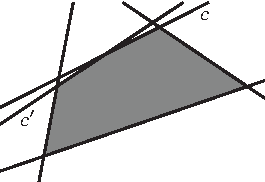
\includegraphics{figures/almostRedundant.pdf}
	\caption{Both inequalities $c$ and $c'$ are almost redundant, but only one of them can be removed from the system.}
	\label{fig:almostRedundant}
\end{figure}

However, we still let the checkers examine whether the inequalities are almost redundant (see \eqref{eq:almostRed}) and report this back to the manager who stores these. After having examined all the needed inequalities by use of parallel redundancy checkers, we then go through and check the almost redundant ones sequentially with a single redundancy checker, and remove - in turn - the ones that are still almost redundant. For the example in Figure~\ref{fig:almostRedundant} this would mean that which ever of $c$ and $c'$ is examined first is also removed, while the other is not.

The checkers also check and report on inequalities for which the optimization of its left hand side resulted in a bad condition number (also known as $\kappa$-value). This number is a measure for how much (small) differences in the input value (i.e. the coefficients and right-hand-side of the (in)equalities) effects the value of output (i.e. the found optimal value); see {e.g. \cite{numAnalysis}}. Essentially, the larger this number is, the less we can trust the result. We have chosen a threshold $\mathcal{K}$ that gives the limit for when we can trust the result. As the system gets smaller due to the removal of redundant inequalities, inequalities might be reexamined with a lower $\kappa$-value as a result, and therefore we also re-examine the inequalities that resulted in a bad $\kappa$-value when they were checked by the parallel redundancy checkers. 
Finally we also reexamine inequalities, for which the lp-solver was not able to solve the optimization of its left-hand-side.

The pseudocode for the redundancy checkers is listed in Algorithm~\ref{alg:checker}, and the pseudocode for the manager is listed in Algorithm~\ref{alg:manager}. 
When the manager receives results from the checkers (via calls to \Call{ManageResult}{} in line~\ref{line:manageResult} in Algorithm~\ref{alg:manager}), it finishes handling one call before handling the next call. %For the parallel checkers, as explained it is important to only check for strict redundancy (well, it is important that only strictly redundant inequalities are removed since otherwise the result can be incorrect due to two parallel checkers removing/reporting each their ``almost redundant'' inequality redundant). When the inequalities are checked sequentially, we can also remove ``almost redundant'' inequalities.

\begin{algorithm}[htbp]
\caption{Initializing and running a redundancy checker. A checker can either check for true redundancy (used when doing concurrent redundancy checks) or not, in which case it checks for ``almost redundancy'' (for doing sequential redundancy checks).}\label{alg:checker}
\begin{algorithmic}[1]
\Function{Solve}{Manager $m$, (In)equality system $S$, $c\in S$, boolean $\mi{truely}$}
	\State $S'\gets S$, $c'\gets c$, $\mathit{reds}\gets \emptyset$
	\While{$c' \neq $ \nul}
		\State Remove $\mi{reds}$ and $c'$ from $S'$
		\State $\mathit{max} \gets \max\set{\vea(c')\cdot\ve{r}}{\ve{r}\in \feas(S')}$
		\State Inspect solution:
		\Indent
			\State $\mathit{red}\gets \false, \mathit{resolve}\gets \false$
			\State $\kappa\gets \Call{GetConditionNumber}{\null}$
			\If{$\mathit{truely}$}
				\State $\mi{red} \gets \Call{IsTruelyRedundant?}{\mathit{max}, \rhs(c')}$ and $\kappa\leq \mathcal{K}$
				\State $\mathit{resolve} \gets \Call{IsAlmostRedundant?}{\mathit{max}, \rhs(c')}$
			\Else
				\State$\mi{red} \gets \Call{IsAlmostRedundant?}{\mathit{max}, rhs(c')}$ and $\kappa\leq\mathcal{K}$
			\EndIf
			\State $\mathit{resolve} \gets \mathit{resolve}$ or $\kappa>\mathcal{K}$ or \Call{Unsolved?}{\null}
		\EndIndent
		\If{$\neg \mathit{red}$}
			\State Add $c'$ to $S'$
		\EndIf
		\State $(c', \mi{reds})\gets m.\Call{ManageResult}{c', \mathit{red}, \mathit{resolve}}$
	\EndWhile
	\State\Return
\EndFunction
\Statex
\Function{IsTruelyRedundant?}{$\mathit{max}, \mathit{rhs}$}
	\State\Return $\mathit{max} \leq \mathit{rhs}$
\EndFunction
\Statex
\Function{IsAlmostRedundant?}{$\mathit{max}, \mathit{rhs}$}
		\State\Return ( $\mathit{rhs} = 0$ and $\mathit{max} \leq \epsilon'$) or 
				$\mathit{max} \leq \mathit{rhs} + \epsilon\cdot |\mathit{rhs}|$
\EndFunction
\end{algorithmic}
\end{algorithm}

We notice that the inequalities that should be checked for redundancy is a subset of (in)equalities in $S$. Essentially, these should be the new inequalities added to the system after each FM-elimination as described earlier. However, the function is implemented such that it is also possible to check the whole system for redundant inequalities.

\begin{algorithm}[htbp]
\caption{Managing the redundancy checkers. First a concurrent redundancy check is performed, followed by a sequential redundancy check. It is assumed that $C'$, $\mathit{reds}$ and $\mathit{resolves}$ can be accessed by any of the manager's functions in this algorithm.}\label{alg:manager}
\begin{algorithmic}[1]
\Function{RemoveRedundancy}{System $S$, inequalities $C\subseteq S\setminus\eqs(S)$, number of checkers $k$}
	\State $S'\gets S,\; C'\gets C,\; \mathit{reds} \gets \emptyset,\; \mathit{resolves} \gets \emptyset$, $\mi{checkers} \gets \emptyset$ 		
\State Do parallel redundancy check:
\Indent
	\DoPar{ $i\gets 1$ to $\min\{k,|C'|\}$}
		\State Add new checker $t$ to $\mi{checkers}$
		\State Call $t.\Call{Solve}{\texttt{this}, S', \textsc{NextIneqToCheck}(), \true}$ 
	\doParUntil{all checkers in $\mi{checkers}$ have returned}
\EndIndent
\Statex
\State $S'\gets S'\setminus reds,\; C'\gets \mi{resolves},\; \mathit{reds} \gets \emptyset,\; \mathit{resolves} \gets \emptyset$
\State Do sequential redundancy check:
\Indent
	\If{$C'\neq \emptyset$}
		\State $t\gets $ new checker, $\mi{checkers} \gets \{t\}$ 		
%	\State $\Call{Initialize}{S'\setminus \mathit{reds}, \mathit{agains}, 1}$
		\State Call $t.\Call{Solve}{\texttt{this}, S', \textsc{NextIneqToCheck}(), \false}$		
	\EndIf
\EndIndent
\State \Return $S'\setminus \mi{reds}$ 
\EndFunction
\Statex
\Function{NextIneqToCheck}{\null}
		\If{ $C'=\emptyset$ }
			\State\Return \nul
		\Else
			\State $c \gets$ first inequality from $C'$
			\State Remove $c$ from $C'$
			\State \Return $c$
		\EndIf
\EndFunction
\Statex
\Function{ManageResult}{Inequality $c$, boolean $red$, boolean $resolve$}\label{line:manageResult}
	\If{$red$}
		\State Add $c$ to $\mathit{reds}$
	%	\State (Tell all the other checkers that $ie$ is redundant)
	\ElsIf{$resolve$}
			\State Add $c$ to $\mathit{resolves}$ 
	\EndIf
	\State \Return $(\Call{NextIneqToCheck}{\null}, \mi{reds})$
\EndFunction
\end{algorithmic}		
\end{algorithm}
%
\subsection{Combining strategies}
For projecting an (in)equality system we combine the various strategies described so far.
We use \Call{Solve}{} from Algorithm~\ref{alg:solve} to find the projection of $S$ w.r.t. $Y\subseteq \VAR(S)$. The method \Call{Project}{} is presented below in Algorithm~\ref{alg:project}. It consists of steps of preprocessing the system, doing Gauss-elimination and doing FM-elimination on the system. After each FM-elimination of a variable some (timewise) ``cheap'' preprocessing steps are done, and we also make sure to remove linearly dependent (in)equalities as well. 
Hence \Call{CleanUp}{} consists of %the (timewise) ``cheap'' preprocessing steps plus \Call{RemoveQuasiIneqs}{}, i.e. 
Algorithm~\ref{alg:prep} minus the calls to \Call{ForcedByBounds}{} and \Call{RemoveLessStrictIneqs}{}.
The reason we do not simply use \Call{Preprocess}{} is that the two above mentioned subprocedures in experience 
are more time consuming than the others and prior results showed a too little effect compared to the time taken.

After this, we remove redundant inequalities (we check only the newly added inequalities) using \Call{RemoveRedundancy}{} from Algorithm~\ref{alg:manager}. 
In \Call{RemoveRedundancy}{}, each step of doing parallel or sequential redundancy checks, respectively, are potentially repeated a number of times (or until the system does not change) depending on the values in the considered model, since ``off''-numbers (according to experience) are more likely to cause bad $\kappa$-values. If there are many inequalities resulting in bad $\kappa$-values, we would then like to test them again (after other redundant inequalities have been removed), since the removal of other inequalities can lead to a better $\kappa$-value when the inequality is re-evaluated.    
Due to the sometimes large number of inequalities that we do not know the redundancy staus of (because of a bad $\kappa$-value, that do not change during the repeated checks for redundancy), in some runs of the method we also start the FM-elimination-step in \Call{Project}{} with a full sequential redundancy check.

\begin{algorithm}\caption{Overview of the method for projecting the variables $Y$ from an (in)equality system  $S$.}\label{alg:project}
\begin{algorithmic}[1]
\Function{Project}{S,Y}
	\State $S'\gets S$
	\State $S'\gets\Call{Preprocess}{S',Y}$\Comment See Algorithm~\ref{alg:prep}
	\State $S'\gets\Call{Gauss-Elim}{S',Y}$\Comment See Algorithm~\ref{alg:Gauss} 
	\State $S'\gets \Call{FM-Elim*}{S',Y}$\Comment FM-elimination with redundancy removal (see below)
\EndFunction
\Statex
\Function{FM-Elim*}{$S,Y$}
	\State  $S'\gets S$, $Y'\gets Y$
	\While{ $Y'\neq \emptyset$ }
		\State $x\gets$ \Call{ChooseVariableToDelete}{$Y'$, $S'$}
		\State $S''\gets(\mi{Zero}_{S'}(x))_{\VAR(S')\setminus\{x\}}$
		\State $S' \gets$ \Call{FM-ElimVar}{$S'$, $x$} \Comment Algorithm~\ref{alg:FMBasic}
		\State Remove $x$ from $Y'$
		\State $S'\gets\Call{CleanUP}{S',Y}$
	%	\State $S'\gets \Call{RemoveQuasiIneqs}{S',Y}$
		\State $S'\gets \Call{RemoveRedundancy}{S', S'\setminus S'', \text{available threads}}$ 	\Comment Algorithm~\ref{alg:manager}\label{ln:projx}
	\EndWhile
	\State \Return $S'$
\EndFunction
\end{algorithmic}
\end{algorithm}
%
\subsection{Decomposition}\label{sec:decomp}
Given the theoretical complexity of the Fourier\--Motzkin\--elimination procedure, we might not have great hope of using this to eliminate a large number of variables from a very large (in)equality system, at least not if the values of the (in)equalities are randomly generated.
%However, we are looking to take advantage of the build-in structure of our problem.
%
However, given an (in)equality system coming from a natural occurring problem, it is common that the constraints are \emph{block structured} \cite{williams}, where groups of constraints are ``local'' for each subdomain of the problem, while other ``global'' or ``transverse'' constraints involve many or all of the local subdomains (see Figure~\ref{fig:decomp1}). We will in the following assume that the given problem has a block structure and exploit this fact. 

Given a problem with block structure, the dense, ``transverse'' (in)equalities are problematic for Fourier-Motzkin-elimination, especially when they use variables that should not be eliminated, and particularly when they are equalities. 
Every time a variable in a transverse equality is eliminated, all the ``local'' (in)equalities using the variable \emph{will be combined} with one of the two inequalities corresponding to the transverse equality. The result is that we get a large number of inequalities using all the variables of the large transverse equality \emph{and} the variables from the local (in)equalities. Thus, not only do we increase the size of the problem, we also make it (much) more dense, both making the rest of the elimination process more time-consuming, and also increasing the time spend on finding redundant inequalities.
%
{Below we show how to avoid this.}

\begin{figure}
	\centering
		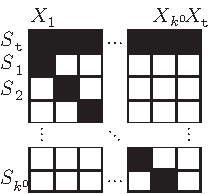
\includegraphics{figures/decomp1B2.pdf}
	\caption{Separation of the (in)equalities of an (in)equality system into local parts and a transverse part. 
	The figure shows the coefficient matrix for the system, where non-zero sections have been colored black.}
	\label{fig:decomp1}
\end{figure}

%%%%%%%%%%%%%%%%%%%%%%%%%%%%%%%%%%%%%%%%%%%%%%%%%%%%%%%%%%%%%%%%%%%%%%%%%%%%%%%%%
\subsubsection{Separating the (in)equality system}
If possible, it would be an advantage to be able to separate our (in)equality system into a (preferably large) number of smaller (in)equality systems that have ``nothing in common'', meaning that there is no overlap between the sets of variables being used in the different subsystem. If this can be done, we can then solve each subsystem separately in parallel after which the resulting systems can be combined (see Lemma~\ref{lm:projection} item \ref{lm:1.1}). As long as each subsystem is sufficiently small (such that it is can be projected in ``reasonable'' time) this may turn an insurmountable large problem into a projectable one. 
However, this is not always possible to do. Nonetheless, using the block structure to decompose the system into smaller subsystems with only little interaction by separating the system's (in)equalities can still be useful. 
 
We therefore consider $k^0$ disjoint subsets of $\VAR(S)$ - $X_1, X_2,\ldots, X_{k^0}$ - and let $X_{\texttt{t}}\odef \VAR(S)\setminus \var(\cup_{1\leq i\leq k^0}X_i)$. For each $i\in\{1,\ldots, k^0\}$ we define $S_i$ to be the (in)equality system that only uses variables in $X_i$, i.e. $S_i \odef \set{c\in S}{\var(c)\subseteq X_i}$, and we let $S_\texttt{t} = S\setminus \cup_{1\leq i \leq k_0}S_i$ be the system consisting of the rest of the (in)equalities. 

The result is that we have divided the system into $k^0$ \emph{local} parts with disjoint sets of used variables, and a \emph{transverse} part that contains (in)equalities using variables from more than one of the other local parts. 

Our (in)equality system can thus be illustrated as in Figure~\ref{fig:decomp1}.

It should be noticed that in general, this can be done in many ways, but in our case - and in many common cases - there is a natural way in which the local parts/local variables present themselves. %For our particular case, many of the constraints are naturally concentrated around stowage of each location while a few constraints traverse several locations, such as the hydrostatic constraints or the constraint defining the type variable.
   
We likewise notice that for any (in)equality system, such partitions of variables and (in)equalities will always exist though they might not be very useful in practice; 
for any $X\subseteq \VAR(S)$, we can make a partition of the (in)equalities as desired, $S = \set{c\in S}{\var(c)\subseteq X}\,\dot\cup \set{c\in S}{\var(c)\not\subseteq X}$.
Intuitively, though, we have a better chance of success if $S_\texttt{t}$ is as small as possible, as well as each $S_i$ and/or $X_i$.

\begin{example}\label{ex:1}
To illustrate, let us consider the (in)equality system $S$ consisting of the following (in)equalities from which we want to eliminate all variables but $u$, % and $u'$, 
which is defined as a sum %, respectively a weighted sum, 
of the variables $x_1, y_1, x_2, y_2, x_3, y_3$:
\begin{gather*}
\mathit{sum}: -u + x_1 + y_1 + x_2 + y_2 + x_3 + y_3= 0\\
%\mi{wSum}&: -u' + x_1 + 2\cdot y_1 + x_2 + 2\cdot y_2 + x_3 + 2\cdot y_3 = 0\\ 
S_1: \left\{ \begin{array}{ll}x_1 + 2 \cdot y_1 &\leq 2\\
															 -x_1 &\leq 0\\
															 -y_1 &\leq 0\end{array}\right.,\qquad
S_2 : \left\{ \begin{array}{ll} -x_2 - 3\cdot y_2 &\leq 1\\
																 x_2 &\leq 0\\
																 y_2 &\leq 0\end{array}\right.,\qquad
S_3 : \left\{ \begin{array}{ll} -x_3 + y_3 &\leq 1\\
																 2\cdot x_3 - y_3 &\leq 0\\
																 -y_3 &\leq 0\end{array}\right..
%\mathit{sum}&: -u_1 + x_1 + x_2 + y_1 + y_2 + z_1 + z_2= 0\\
%\mi{wSum}&: -u_2 + x_1 + 2\cdot x_2 + y_1 + 2\cdot y_2 + z_1 + 2\cdot z_2 = 0\\ 
%S_x &: \left\{ \begin{array}{ll}x_1 + 2 \cdot x_2 &\leq 2\\
%															 -x_1 &\leq 0\\
%															 -x_2 &\leq 0\end{array}\right.\\
%S_y &: \left\{ \begin{array}{ll} -y_1 - y_2 &\leq 1\\
%																 y_1 &\leq 0\\
%																 y_2 &\leq 0\end{array}\right.\\
%S_z &: \left\{ \begin{array}{ll} -z_1 + z_2 &\leq 1\\
%																 2\cdot z_1 - z_2 &\leq 0\\
%																 -z_2 &\leq 0\end{array}\right..
\end{gather*}
$S_1$, $S_2$ and $S_3$ are ``local'' subsystems only dealing with variables from $\{x_1,y_1\}$, $\{x_2, y_2\}$ and $\{x_3,y_3\}$, respectively. On the other hand, the equality defining $u$, %and $u'$, 
$\mathit{sum}$, % and $\mi{wSum}$, are 
is a transverse equality. When eliminating any $x$ or $y$ variable, the system will be added (in)equalities using all variables (except the eliminated one) due to combinations with $\mi{sum}$. % and $\mi{wSum}$.
\end{example}

\paragraph{Introducing auxiliary variables}
As previously mentioned it is preferable to perform elimination on a (local) subsystem such that only (in)equalities naturally ``belonging'' to that subsystem are produced, meaning that added (in)equalities uses no variables from other (local) subsystems. 
This can be achieved by the use of auxiliary variables.

Assume that $c:\sum_{x\in \VAR(c)} \coef(x,c)\cdot x \odot_c \rhs(c)$ belongs to $S_\texttt{t}$.  
For all $1\leq i \leq k^0$ we then define a variable\footnote{{Formally, we define the value of a variable in $\xx\setminus \VAR(S)$ which we will rename $z^0_{c,i}$, and so forth with all the following, defined variables}.}, $z_{c,i}^{0} \odef \sum_{x\in X_i}  \coef(x,c)\cdot x$, which can be written as an equality over $X_i\cup \{z^0_{c,i}\}$ as
\begin{equation}\label{eq:z^0_{c,i}}
\mathit{Def}(z^0_{c,i}): -z_{c,i}^{0} + \sum_{x\in X_i}  \coef(x,c)\cdot x = 0.
\end{equation}
Since $\VAR(S) = X_1 \,\dot{\cup}\; \ldots \,\dot{\cup}\; X_{k^0} \,\dot{\cup}\; X_{\texttt{t}}$ and $\coef(x,c)=0$ for $x\in \VAR(S)\setminus \var(c)$, we therefore have that 
\begin{align*}
\sum_{x\in \VAR(c)} \coef(x,c)\cdot x  
&= \sum_{x\in \VAR(S)} \coef(x,c)\cdot x \\
&= \big(\sum_{1\leq i \leq k^0}\big(\sum_{x\in X_i} \coef(x,c)\cdot x\big)\big) + \sum_{x\in X_{\ttt}}\coef(x,c)\cdot x\\
&= \big(\sum_{1\leq i\leq k^0}z^0_{c,i}\big)+\sum_{x\in X_\texttt{t}}\coef(x,c)\cdot x,
\end{align*}
which means that using the $z^0_{c,i}$-variables, $c$ can be rewritten as an (in)equality over $\cup_{1\leq i\leq k_0}\{z^0_{c,i}\}\cup X_\ttt$ as  
\begin{equation}\label{transEq}
c^0_{decp}:\big(\sum_{1\leq i \leq k^0} z_{c,i}^{0}\big) + \sum_{x\in X_\texttt{t}}\coef(x,c)\cdot x \odot_c \rhs(c).
\end{equation}
From construction it therefore follows that values for $x\in \VAR(S)$ that satisfies $c$ can be extended with values for all $z^0_{c,i}$ such that $c^0_{decp}$ and all the defining equalities (from \eqref{eq:z^0_{c,i}}) are satisfied, and vice versa, if the latter (in)equalities are all satisfied then satisfying values for the variables in $X$ will also satisfy $c$. That is,
\begin{equation}\label{eq:projz}
\feas(c)=\proj_{\cup_{1\leq i\leq k^0}\{z^0_{c,i}\}}\big(\feas(\{c^0_{decp}\}\cup\bigcup_{1\leq i\leq k^0}\{\mi{Def}(z^0_{c,i})\})\big).
\end{equation}
Using auxiliary variables for all $c\in S_\texttt{t}$ as above and adding the defining equalities $\mi{Def}(z^0_{c,i})$ to the subsystem where they belong according to their variables, we can divide the (in)equality system $S$ into a number of (in)equality systems, $S^0_1,\ldots, S^0_{k^0}, S^0_\texttt{t}$, 
as described in the pseudocode below. 

\begin{algorithm}
\caption{Separating an (in)equality system $S$ according to a list of disjoint sets of variables $\mathbb{X}=(X_1, X_2, \ldots, X_{k^0})$, where each $X_i\subseteq \VAR(S)$}\label{alg:separate}
\begin{algorithmic}[1]
\Function{SeparateIneqs}{$S$, $\mathbb{X}=(X_1, X_2, \ldots, X_{k^0})$}
\State $S_\ttt \gets \set{c\in S}{\var(c)\not\subseteq X_i\text{ for any } i}$
\For{$i\gets 1$ to $k^0$}
	\State $S^0_i \gets \set{c_{X_i}}{c\in S, \var(c)\subseteq X_i}$%\set{c_{X_i'}}{c\in S, \var(c)\subseteq X_i}$
\EndFor
\State $S^0_\ttt\gets \emptyset$ %empty set of (in)equalities over $X_\ttt^0$
\ForAll{$c\in S_\ttt$}
	\For{$i\gets 1$ to $k^0$}
		\State Add $\mathit{Def}(z^0_{c,i}): -z^{0}_{c,i} + \sum_{x\in X_i} \coef(x,c)\cdot x = 0$ to $S_i^0$
	\EndFor
	\State Add $c^0_{decp}: (\sum_{1\leq i\leq k^0} z_{c,i}^0) +\sum_{x\in X_\texttt{t}}\coef(x,c)\cdot x \odot_c \rhs(c)$ to $S^0_\texttt{t}$ 
\EndFor
\State\Return ($(S^0_1,\ldots, S^0_{k^0}), S^0_\texttt{t}$)
\EndFunction
\end{algorithmic}
\end{algorithm}

The (in)equality system consisting of the union of the systems $S^0_1,\ldots, S^0_{k^0}, S^0_\texttt{t}$ will be referred to as the \emph{separated system from $S$}, written $\mi{sep}(S)$. This can be illustrated as in Figure~\ref{fig:decomp3}. For ease of notation we let $Z^0 \odef \cup_{1\leq i\leq k^0}\set{z^0_{c,i}}{c\in S_\ttt}$. We notice that for each constructed system $S^0_i$ we have that $\VAR(S^0_i)\subseteq X_i\cup Z^0$ and $\VAR(S^0_t) = X_\ttt \cup Z^0$. 

\begin{figure}[htbp]
	\centering
		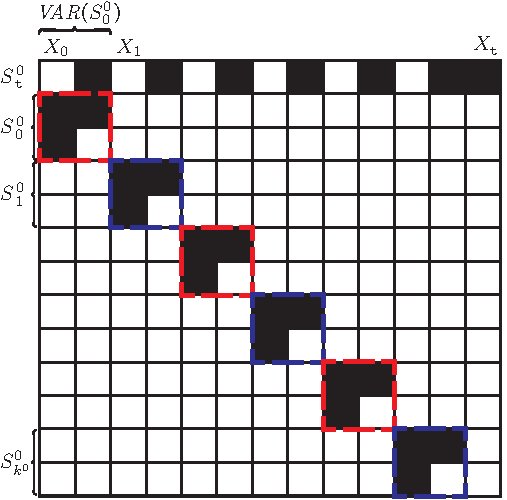
\includegraphics[scale = 0.8]{figures/decomp3B.pdf}
	\caption{The separated system from the system in Figure~\ref{fig:decomp1}. Auxiliary variables are used to prevent local constraints from different local parts to instantly ``mix'' when their variables are eliminated. Each system $S^0_i$, however, only corresponds to the system encased in coloured boxes.}
	\label{fig:decomp3}
\end{figure}
%
\begin{example}\label{ex:2}
Consider again the (in)equality system $S$ from Example~\ref{ex:1}. As explained, separating $S$ introduces auxiliary variables to prevent the immediate mix of variables from $\var(S_1)$, $\var(S_2)$ and $\var(S_3)$ in new inequalities when any of the variables are eliminated. This is done by defining $u$ as the sum of three auxiliary variables, $z_1$, $z_2$ and$ z_3$, which in turn are defined as the sum of the variables in each respective subsystems. Hence $\mi{sep}(S)$ is the following system.
\begin{gather*}
\mathit{sum}^0_{decp}: -u + z_1 + z_2 + z_3 = 0\\
%\mi{wSum}^0&: -u' + z_1' + z_2' + z_3' = 0\\ 
S_1^0 : \left\{ \begin{array}{ll}-z_1 + x_1 + y_1 &= 0\\
%																-z_1' + x_1 + 2\cdot y_1 &= 0\\
															  x_1 + 2 \cdot y_1 &\leq 2\\
															 -x_1 &\leq 0\\
															 -y_1 &\leq 0\end{array}\right.,\qquad
S_2^0 : \left\{ \begin{array}{ll} -z_2 + x_2 + y_2 &= 0\\
%																-z_2' + x_2 + 2\cdot y_2 &= 0\\
																-x_2 - 3\cdot y_2 &\leq 1\\
																 x_2 &\leq 0\\
																 y_2 &\leq 0\end{array}\right.,\qquad
S_3^0 : \left\{ \begin{array}{ll} -z_3 + x_3 + y_3 &= 0\\
%																-z_3' + x_3 + 2\cdot y_3 &= 0\\
																 -x_3 + y_3 &\leq 1\\
																 2\cdot x_3 - y_3 &\leq 0\\
																 -y_3 &\leq 0\end{array}\right..
%\mathit{sum}^0&: -u_1 + x + y + z = 0\\
%\mi{wSum}^0&: -u_2 + x' + y' + z' = 0\\ 
%S^0_x &: \left\{ \begin{array}{ll}-x + x_1 + x_2 &= 0\\
																%-x' + x_1 + 2\cdot x_2 &= 0\\
																%x_1 + 2 \cdot x_2 &\leq 2\\
															 %-x_1 &\leq 0\\
															 %-x_2 &\leq 0\end{array}\right.\\
%S^0_y &: \left\{ \begin{array}{ll} -y + y_1 + y_2 &= 0\\
																%-y' + y_1 + 2\cdot y_2 &= 0\\
																 %-y_1 - y_2 &\leq 1\\
																 %y_1 &\leq 0\\
																 %y_2 &\leq 0\end{array}\right.\\
%S^0_z &: \left\{ \begin{array}{ll} -z + z_1 + z_2 & = 0\\
																%-z' + z_1 + 2\cdot z_2 &= 0\\
																	%-z_1 + z_2 &\leq 1\\
																 %2\cdot z_1 - z_2 &\leq 0\\
																 %-z_2 &\leq 0\end{array}\right..
\end{gather*}
When we eliminate $x_1, y_1, x_2, y_2, x_3$ and $y_3$ from $S'$, we do not ``mix'' the local subsystems; this only happens when $z_1$, $z_2$ and $z_3$ 
% $z_1'$, $z_2'$ and $z_3'$ 
 afterward are eliminated. 

Furthermore, when eliminating $x_1$ and $y_1$, we only need to do this with respect to the system $S^0_1$ (and similar for $\var(S^0_2)$ and $\var(S^0_3)$). The resulting projections from $\prs_{\{x_1, y_1\}}(S^0_1)$, $\prs_{\{x_2, y_2\}}(S^0_2)$ and $\prs_{\{x_3, y_3\}}(S^0_3)$, respectively, can then be added to $\mi{sum}^0$ %and $\mi{wSum}^0$ 
from which $z_1$, $z_2$ and $z_3$ 
% $z_1'$, $z_2'$ and $z_3'$ 
can then be eliminated. %In general, this further improves the runtime of some of the subprocedures in our projection algorithm since each subsystems $S^0_1$, $S^0_2$ and $S^0_3$ will be relatively smaller than the overall system.  
\end{example}

In the end, the result is that each set $S_i^0$ now have one more (in)equality for each $c \in S_\ttt$ %\red{containing variables from $X_i$} 
compared to the original $S_i$, and the number of variables in $\var(S_i^0)$ has increased with the same amount compared to $X_i$.
But, more importantly, now $|\var(S_i^0)\cap \var(S^0_\ttt)|$ equals $|S_\ttt|$, and eliminating variables in $X_i\cap Y$ will only produce (in)equalities whose set of variables is disjoint from the variable sets of the other local (in)equality systems.
Furthermore, eliminating the $z^0_{c,i}$-variables from the separated system 
will give us a system equivalent to the original system. 
Hence, eliminating the variables in $Y\subseteq \VAR(S)$ from the original system is equivalent to eliminating $Y$ and the defined $z$-variables, that is 
\[
\prs_Y(S) = \prs_{Y\cup Z^0}(\mi{sep}(S)).
\]
This follows from Lemma~\ref{lm:separating} below since by construction $\VAR(S)\setminus Y = \VAR(\mi{sep}(S))\setminus (Y\cup Z^0).$
\begin{restatable}{lemma}{separating}\label{lm:separating}
\[
\proj_Y\big(\feas(S)\big)=\proj_{Y\cup Z^0}\big(\feas(\mi{sep}(S))\big).
\]
\end{restatable}
\begin{proof}
See Appendix
\end{proof}

\subsubsection{Splitting transverse constraints}
Separating the system as described above helps preventing the (in)equalities becoming too dense when eliminating variables from the local parts. However, we also need to eliminate the defined variables in $Z^0$, which there might be many of. Using auxiliary variables in a way similar to the one described above, we would therefore like to split the variables in $Z^0$ into groups and use auxiliary variables to prevent subsystems ``mixing'' with each other. Potentially, projecting the subsystems will again result in manageable systems that can then be put together.

We will exploit the fact that if the left-hand-side of a transverse (in)equality in $S^0_\texttt{t}$ consists of a sum of many terms, it can always be rewritten as a sum of fewer terms by use of auxiliary variables. For example
\begin{align*}
z^0_{c,1} + z^0_{c,2} + \ldots + z^0_{c,k^0} &=
(z^0_{c,1} + z^0_{c,2}) + \ldots + (z^0_{c,k^0-1} + z^0_{c, k^0}) \\
&= z^1_{c,1} + \ldots + z^1_{c,k^1},
\end{align*}
where $z^1_{c,1} = z^0_{c,1} + z^0_{c,2},\; \ldots,\; z^1_{c,k^1}=z^0_{c,k^0-1} + z^0_{c,k^0}$. The latter sum can then again be rewritten into a sum of fewer terms, and so on.

\begin{example}
If we take the (separated) (in)equality system $\mi{sep}(S)$ from Example~\ref{ex:2}, the variable $u$ (which we want to keep) is now defined as a sum of three other variables ($z_1, z_2, z_3$) instead of the former six variables. %, and similarly for $u_2$. 
Of course, this example is very small and a further splitting of the transverse constraints is most likely not necessary, but for the purpose of illustration, we can further split $\mi{sum}$ %and $\mi{wSum}$ 
such that the system obtained consists of the following (in)equalities (drawn in a tree structure): 

\begingroup
\centering
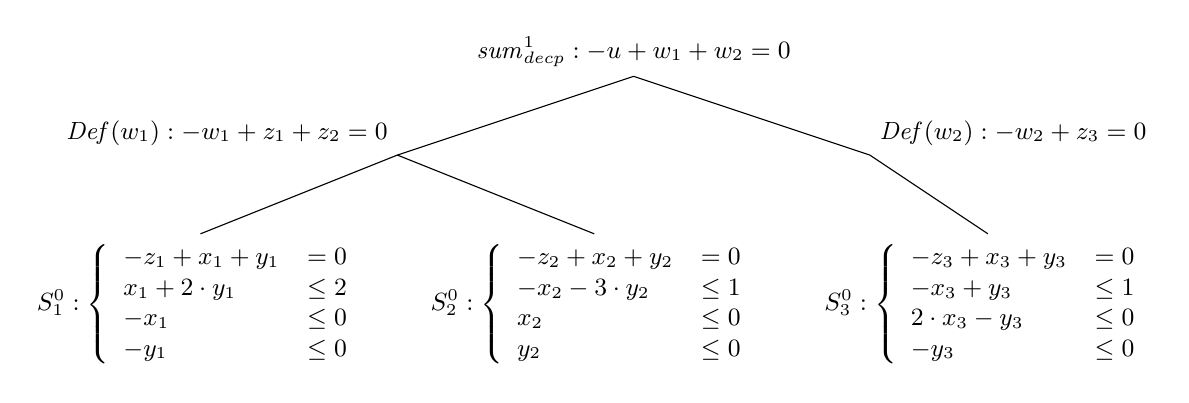
\begin{tikzpicture}
\node [above] at (6.5,3) {\small{$\mathit{sum}^1_{decp}: -u + w_1 + w_2 = 0$}};
%																									\mi{wSum}^1&: -u_2 + v' + w' = 0
\draw [thin] (3.5,2) -- (6.5,3) -- (9.5,2);
\node [above left] at (3.5,2) {\small{$\mi{Def}(w_1): %\left\{ \begin{array}{ll} 
																-w_1 + z_1+ z_2 = 0$}};
																 %-u'+ w_1' + w_2'&= 0
																%\end{array}\right.$}};
\draw [thin] (1,1) -- (3.5,2) -- (6,1);
\node [above right] at (9.5,2) {\small{$\mi{Def}(w_2): %\left\{ \begin{array}{ll} 
															-w_2 + z_3 = 0$}};
																% -w' + z'&= 0
															%	\end{array}\right.$}};
\draw [thin] (9.5,2) -- (11,1);
\node [below] at (1,1) {\small{$S^0_1: \left\{ \begin{array}{ll}-z_1 + x_1 + y_1 &= 0\\
																%-z_1' + x_1 + 2\cdot y_1 &= 0\\
																x_1 + 2 \cdot y_1 &\leq 2\\
															 -x_1 &\leq 0\\
															 -y_1 &\leq 0\end{array}\right.$}};
\node [below] at (6,1) {\small{$S^0_2: \left\{ \begin{array}{ll} -z_2 + x_2 + y_2 &= 0\\
																%-z_2' + x_2 + 2\cdot y_2 &= 0\\
																 -x_2 - 3\cdot y_2 &\leq 1\\
																 x_2 &\leq 0\\
																 y_2 &\leq 0\end{array}\right.$}};
\node [below] at (11,1) {\small{$S^0_3: \left\{ \begin{array}{ll} -z_3 + x_3 + y_3 & = 0\\
																 %-z_3' + x_3 + 2\cdot y_3 &= 0\\
																 -x_3 + y_3 &\leq 1\\
																 2\cdot x_3 - y_3 &\leq 0\\
																 -y_3 &\leq 0\end{array}\right.$}};
\end{tikzpicture}
\endgroup

To eliminate all variables but $u$ %and $u'$ 
from the system, we first find projections $E^0_1\in \prs_{\{x_1, y_1\}}(S^0_1)$, $E^0_2\in \prs_{\{x_2, y_2\}}(S^0_2)$, $E^0_3\in \prs_{\{x_3, y_3\}}(S^0_3)$. Then we find projections $E^1_1\in \prs_{\{z_1,z_2\}}(E^0_1\cup E^0_2\cup %S^1_1)$ 
\{\mi{Def}(w_1)\})$ and $E^1_2\in \prs_{\{z_3\}}(E^0_3\cup %S^1_2)$ 
\{\mi{Def}(w_2)\})$ and then we find a projection $E\in \prs_{\{w_1, w_2\}}(E^1_1\cup E^1_2 \cup \{\mi{sum}^1\})$.%,\mi{wSum}^1\})$.
\end{example}
%
To further divide the transverse (in)equalities, we use an ``appropriate'' partition $\mathbb{P}^1 = (P^1_1, \ldots, P^1_{k^1})$ of the indices of the local parts, $\{1,\ldots, k^0\}$.
What is ``appropriate'' can vary, depending e.g. on the number of (in)equalities and variables in the subproblems as well as the underlying structure (if any) of the original problem. %In our case, we have used parts that have between 1 and 3 elements (see Section~\ref{sec:testResults}). %in our particular case, we often make the parts have between 1 and 3 elements, depending on the underlying structure of the ship. 
For each transverse (in)equality $c^0_{decp}:(\sum_{1\leq i \leq k^0}z^0_{c,i}) + \sum_{x\in X_{\texttt{t}}}\coef(x,c)\cdot x
\odot_{c}\rhs(c)$ in $S^0_\texttt{t}$ and each part $P^1_i\in \mathbb{P}^1$ we then define a variable to be the sum over the $z^0_{c,j}$-variables, whose index $j$ is in that particular part $P_i$. That is, we define the following equality $\mathit{Def}(z_{c,i}^1)$ over $\{z^1_{c,i}\}\cup\bigcup_{j\in P^i_i}\{z^0_{c,i}\}$.
\begin{equation}\label{eq:z1}
\mathit{Def}(z_{c,i}^1): -z_{c,i}^1 + \sum_{j\in P_i^1} z_{c,j}^{0} = 0.
\end{equation}
%
Using the defined variables we can then substitute in $c^0_{decp}$ to get an (in)equality over $X_\ttt\cup\bigcup_{1\leq i\leq k^1}\{z^1_{c,i}\}$.
\[
c_{decp}^1: (\sum_{1\leq i\leq k^1} z^1_{c,i}) + \sum_{x\in X_{\texttt{t}}}\coef(x,c)\cdot x \odot_c \rhs(c).
\]
Letting $Z^1 \odef \cup_{1\leq i\leq k^1}\set{z^1_{c,i}}{c\in S_\ttt}$ we can now split the newly added (in)equalities into $k^1$ ``variable-disjoint'' and one ``transverse'' (in)equality systems by defining $S^1_i\odef\set{\mi{Def}(z^1_{c,i})}{c\in S^0_\texttt{t}}$ for each $1\leq i\leq k^1$ (i.e. $\VAR(S^1_i) = \bigcup_{c\in S^0_\ttt}\VAR(\mi{Def}(z^1_{c,i}))\subseteq Z^0\cup Z^1$) and $S^1_\texttt{t} \odef \set{c_{decp}^1}{c\in S^0_\texttt{t}}$ (i.e $\VAR(S^1_\ttt) = \bigcup_{c\in S^0_\ttt}\VAR(c^1_{decp}) = X_\ttt\cup Z^1$).

If $\var(c_{decp}^1)$ is still deemed too large, i.e. $k^1$ is too large, we can repeat this step - use a partition of the indices of the previous partition to define and use auxiliary variables - until the (in)equality $c_{decp}^K$ only has a few terms, see Figure~\ref{fig:split}.
%
\begin{figure}
	\centering
		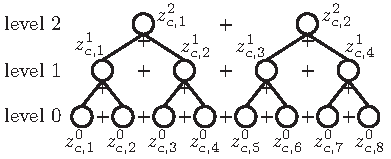
\includegraphics{figures/split.pdf}
	\caption{Splitting a transverse constraint $c^0_{decp}: \sum_{i = 1}^8 z^0_{c,i} + \sum_{x\in X_{\texttt{t}}}\coef(x,c)\cdot x\odot_c \rhs(c)$ in $S_\texttt{t}^0$ from a separated system using the partitions $\mathbb{P}^1 = \{1,2\}\;\dot\cup\{3,4\}\;\dot\cup\{5,6\}\;\dot\cup\{7,8\}$ and $\mathbb{P}^2 = \{1,2\}\;\dot\cup\{3,4\}$. 
	}
	\label{fig:split}
\end{figure}
%
The procedure for splitting the transverse (in)equalities like this according to a partition at a given level $l$ can be described by the following procedure \Call{SplitTransverse}{} in Algorithm~\ref{alg:split}.
%

\begin{algorithm}
\caption{Splitting a transverse (in)equality at the $l$'th level, according to a partition $\mathbb{P}^l$ of the indices of the previous level.}
\label{alg:split}
\begin{algorithmic}[1]
\Function{SplitTransverse}{%Set of transverse (in)equalities $S^0_\texttt{t}$, partition $\mathbb{P}^l = (P^l_1, \ldots, P^l_{k^l})$}
Transverse (in)equalities $S^0_\texttt{t}$, partitions $\mathbb{P}^l = (P^l_1, \ldots, P^l_{k^l})$}
	%\State $X\gets \VAR(S^0_\ttt)\cup \bigcup_{1\leq m\leq l}\set{z^m_{c,i}}{c\in S^0_\ttt}$
	\State $S_\texttt{t}^l\gets \emptyset$% (in)equality system over $X$
	\For{$i\gets 1$ to $k^l$}
		\State $S^l_i \gets \emptyset$ 
		\ForAll{$c\in S_\texttt{t}^0$}
				\State Add $\mathit{Def}(z^l_{c,i}): -z^l_{c,i} + \sum_{j\in P^l_i} z^{l-1}_{c,j} = 0$ to $S^l_i$
		\EndFor
		\State Add $c_{decp}^l: (\sum_{1\leq i\leq k^l} z^l_{c,i}) + \sum_{x\in X_{\texttt{t}}}\coef(x,c)\cdot x \odot_c \rhs(c)$
 to $S_\texttt{t}^l$
	\EndFor
	\State\Return $((S^l_1,\ldots, S^l_{k^l}), S^l_\texttt{t})$
\EndFunction
\end{algorithmic}
\end{algorithm}
%
At each step, we define auxiliary variables in terms of the previous level's auxiliary variables, and then we replace each decomposed transverse inequality from the previous level with another decomposed transverse inequality that uses the new auxiliary variables. The defining equalities are split into groups according to a partition of (the indices of) the previous level's variables.

Due to the definition of the new variables, $Z^l$, and the decomposed (in)equalities at the $l$'th level, it follows that eliminating the $Z^l$-variables from 
the (in)equalities defined thus far gives us an the (in)equality system consisting of all (in)equalities at the previous level; see Lemma~\ref{lm:4} below.

\begin{restatable}{lemma}{lmmmm}\label{lm:4}
\[
\proj_{Z^l}\big(\feas(S^l_\ttt\cup\bigcup_{1\leq i\leq k^l}S^l_i)\big) = \feas(S^{l-1}_\ttt)
\]
\end{restatable}
\begin{proof}
See Appendix.
\end{proof}
%
%%%%%%%%%%%%%%%%%%%%%%%%%%%%%
%%%%%%%%%%%%%%%%%%%%%%%%%%%%
%
\subsubsection*{Solving the (in)equality system exploiting structure}
Having separated the system and split the transverse (in)equalities, we can now solve the original problem, that is, eliminate the variables $Y$ from the (in)equality system $S$. The result will be an (in)equality system, whose feasible region is the projection of $Y$ from $S$, i.e. the system belongs to $\prs_Y(S)$ and will be expressed in the variables $X\setminus Y$. Though, instead of considering the whole system $S$ and eliminating the variables in $Y$ from this set, we will as previously mentioned take advantage of the decomposition of the problem. 

The overall idea of the procedure is to use the constructed decomposition of the (in)equality system to make a tree structure of subsystems where a system $S^l_i$ has the subsystems $S^{l-1}_{j}$ as a child for all $j\in P^l_i$ (see Figure~\ref{fig:treeStructureSs}). The systems corresponding to the subtrees in this structure are then projected recursively (see Figure~\ref{fig:recursiveProjectionEs} later).

{Given that the constraints of a given subproblem \emph{in real life} deals with the same aspect of the problem in question, there is a good chance that the projected subsystem with the aid of some variables significant for that aspect can be expressed in only few constraints. By separating the system and splitting the transverse constraints, which both results in divisions into subproblems, we therefore hope to better take advantage of the structure of the problem.}
\\\\
Firstly, we let $\mathfrak{S}^l_i$ denote the (in)equality system consisting of $S^l_i$ together with all it's descendants in this tree structure, see Figure~\ref{fig:treeStructureSs}. 

\begin{figure}[htbp]
	\centering
		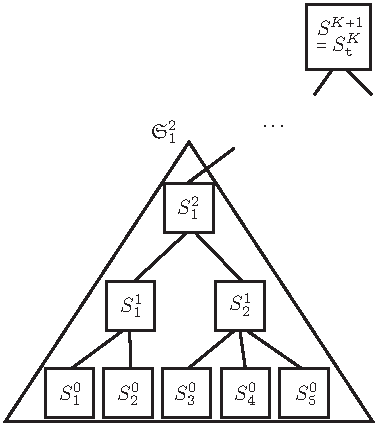
\includegraphics{figures/treeStructureSs.pdf}
	\caption{A part of the tree structure for an (in)equality system $S$. For the partitions it holds that $P^1_1, P^1_2\in \mathbb{P}^1$ where $P^1_1 = \{1,2\}$ and $P^1_2 =\{3,4,5\}$, and $P^2_1\in\mathbb{P}^2$ where $P^2_1=\{1,2\}$.}
	\label{fig:treeStructureSs}
\end{figure}

Letting $k^{K+1}=1$, $P^{K+1}_1 = \{1,\ldots, k^K\}$, and $S^{K+1}_1 = S^K_\ttt$, we formally define $\mathfrak{S}^l_i$ for all $0 \leq l \leq K+1$ and all $1\leq i \leq k^l$ as
\[
\mathfrak{S}^l_i = \left\{\begin{array}{ll}
		S^l_i \cup\bigcup_{j\in P^l_i}\mathfrak{S}^{l-1}_j&\text{if }l>0\\
		S^l_i&\text{if } l=0
\end{array}\right.
\]
Not surprisingly it is easily shown (see Lemma~\ref{lemma2} below) that $\mathfrak{S}^{K+1}$ indeed equals the union of all the defined subsystems.
\begin{restatable}{lemma}{lemmato}\label{lemma2}
\[
S^K_\ttt\cup\bigcup_{1\leq i\leq k^0}S^0_i\cup\ldots\cup\bigcup_{1\leq i\leq k^K} S^K_i = \mathfrak{S}^{K+1}_1
\]
\end{restatable}
\begin{proof}
See Appendix.
\end{proof}
%
\noindent As expected, projecting all $Y$ and $Z$-variables from the final system corresponds to projecting the $Y$ variables from the original system. From this it follows that 
\begin{equation}\label{eq:projYZ}
\prs_Y(S) = \prs_{Y\cup Z^0\cup \ldots \cup Z^K}(\mathfrak{S}^{K+1}_1)
\end{equation}
since $\VAR(S)\setminus Y = \VAR(\mathfrak{S}^{K+1}_1)\setminus(Y\cup Z^0\cup \ldots \cup Z^K)$. 
The following proposition proves the claim more formally.
\begin{restatable}{prop}{propto}\label{prop:2}
\[
\proj_Y\big(\feas(S)\big) = \proj_{Y\cup Z^0\cup \ldots \cup Z^K}\big(\feas(\mathfrak{S}^{K+1}_1)\big) 
\]
\end{restatable}
\begin{proof}
See Appendix.
\end{proof}
%
\noindent To obtain a system from $\prs_Y(S)$, we can therefore instead eliminate all $Y$ and $Z$ variables from the final system. Although this seems more troublesome, we can use the constructed tree structure to project the (in)equality system, such that a subsystem $S^l_i$ is projected by first projecting each of its subtree's systems ($\mathfrak{S}^{l-1}_j$ for $j\in P^l_i$) recursively, add these projections to $S^l_i$ and then finally project the result w.r.t. $(Y\cup Z^{l-1})\cap S^l_i$. See Figure~\ref{fig:recursiveProjectionEs}.

For each $0\leq l\leq K$ and $1\leq i \leq k^l$, we let $\mathfrak{E}^l_i$ be one of the systems in the (recursive) projection of $S^l_i$ and its subsystems (see Figure~\ref{fig:recursiveProjectionEs}). 

\begin{figure}
	\centering
		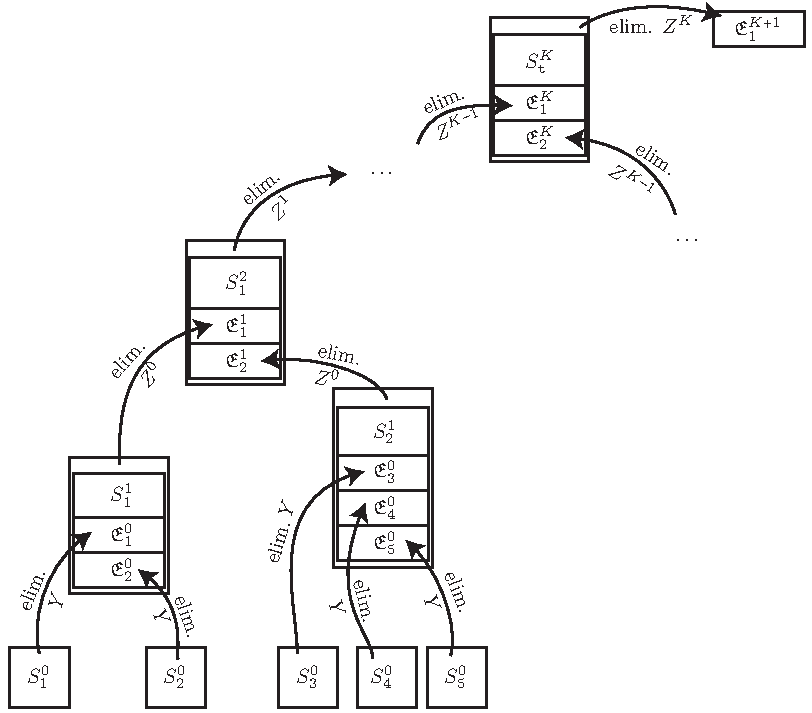
\includegraphics{//fs4.itu.local/redirection/ajspur/Pictures/recursiveProjectionEs.pdf}
	\caption{Using the tree structure from Figure~\ref{fig:treeStructureSs} for an (in)equality system $S$ to recursively project the variables $Y\subseteq \VAR(S)$.}
	\label{fig:recursiveProjectionEs}
\end{figure}

\noindent More formally we define   
\begin{equation}\label{eq:mathfrakE}
\mathfrak{E}^l_i = \left\{\begin{array}{ll}
		\mathit{pick}(\prs_{Z^{l-1}}(S^l_i \cup\bigcup_{j\in P^l_i}\mathfrak{E}^{l-1}
		_j)) &\text{if }l>0\\
		\mathit{pick}(\prs_{Y}(S^l_i))&\text{if } l = 0
\end{array}\right.,
\end{equation}
where $\mathit{pick}: 2^{2^{\ie}}\to 2^{\ie}$ is an arbitrary choice-function, i.e. given a set of (in)equality systems $M$, it returns one of the (in)equality systems in $M$. As it turns out (see Lemma~\ref{lm:picking} later), the specific choice function is irrelevant for our purpose, so for now we just assume this function given.

The proposition below now gives us that projecting the $Y$- and $Z$-variables recursively as given in \eqref{eq:mathfrakE} results in the same as projecting all the variables from the final system. 
%
\begin{restatable}{prop}{proptre}\label{prop:3}
\[
\proj_{Z^{K}\cup \ldots \cup Z^0\cup Y}\big(\feas(\mathfrak{S}^{K+1}_1)\big) = \feas(\mathfrak{E}^{K+1}_1)
\]
\end{restatable}
\begin{proof}
See Appendix.
\end{proof}
%

From Proposition~\ref{prop:2} and Proposition~\ref{prop:3} it follows that $\feas(\mathfrak{E}^{K+1}_1)=\proj_Y\big(\feas(S)\big)$. It then follows from Lemma~\ref{lm:picking} below that the given choice function is irrelevant.

\begin{cor}
No matter in which way the system $\mathfrak{E}^l_i$ is chosen from $\prs_{Z^{l-1}}(S^l_i \cup\bigcup_{j\in P^l_i}\mathfrak{E}^{l-1}_j)$ (for $l>0$) or from $\prs_{Y}(S^l_i)$ (for $l=0$) we have that 
\[
\mathfrak{E}^{K+1}_1 \in \prs_{Y}(S)
\]
\end{cor}
%
\begin{restatable}{lemma}{picking}\label{lm:picking}
Let $p,p':2^{2^\ie}\to 2^\ie$ be such that $p(M),p'(M)\in M$ for all $M\in 2^{2^\ie}$. Then $\mathfrak{E}^l_i(p)\cong\mathfrak{E}^l_i(p')$ for all $0\leq l\leq K+1$ and all $1\leq i\leq k^l$, where
\begin{align*}
\mathfrak{E}^l_i(p) &\odef \left\{\begin{array}{ll}
		\mathit{p}\big(\prs_{Z^{l-1}}(S^l_i \cup\bigcup_{j\in P^l_i}\mathfrak{E}^{l-1}_j(p))\big) &\text{if }l>0\\
		\mathit{p}\big(\prs_{Y}(S^l_i)\big)&\text{if } l = 0
\end{array}\right.,\text{ and }\\
\mathfrak{E}^l_i(p') &\odef \left\{\begin{array}{ll}
		\mathit{p'}\big(\prs_{Z^{l-1}}(S^l_i \cup\bigcup_{j\in P^l_i}\mathfrak{E}^{l-1}_j(p'))\big) &\text{if }l>0\\
		\mathit{p'}\big(\prs_{Y}(S^l_i)\big)&\text{if } l = 0
\end{array}\right..
\end{align*}
\end{restatable}
\begin{proof}
See Appendix.
\end{proof}
%
Below in Algorithm~\ref{alg:solve} we present an algorithm for producing the system $\mathfrak{E}^l_i$ according to the definition in \eqref{eq:mathfrakE} for some choice-function $\mathit{pick}$. As described, this algorithm can then be used to  find a projection of $S$ w.r.t. $Y$. In the algorithm we use the method \Call{Project}{$S',Y'$} as a function that returns a projection of the (in)equality system $S'$ w.r.t. the set of variables $Y'\subseteq\VAR(S')$. This method uses preprocessing, Gauss- and FM-elimination as previously described in Algorithm~\ref{alg:project}. 

\begin{algorithm}
\caption{Projecting the variables $Y$ from an (in)equality system $S$ by decomposing it.
$\mathbb{X}=(X_1,\ldots, X_{k^0})$ is a list of disjoint subsets of $\VAR(S)$, and 
$\mathfrak{P}=(\mathbb{P}^1, \ldots, \mathbb{P}^K)$ is a list of partitions. Each $\mathbb{P}^l$ is a partition of $\{1,\ldots, k^{l-1}\}$, where $k^{i}=|\mathbb{P}^i|$ for $i>0$ and $k^0 = |\mathbb{X}|$.}
\label{alg:solve}
\begin{algorithmic}[1]
\Function{Solve}{System $S$, variables $Y\subseteq \VAR(S)$, variable sets $\mathbb{X}$, partitions $\mathfrak{P}$}
	\State $(\mathbb{S}^0,S_\texttt{t}^0) \gets \Call{SeparateIneqs}{S,\mathbb{X}}$\Comment See Algorithm~\ref{alg:separate}
	\For{$l\gets 1$ to $K$}
		\State $(\mathbb{S}^l,S^l_\texttt{t})\gets\Call{SplitTransverse}{S^0_\texttt{t},\mathbb{P}^l}$ \Comment See Algorithm~\ref{alg:split}
	\EndFor
	\State $\mathbb{S}^{K+1} =(S^K_\texttt{t})$
	\State\Return\Call{Solve-Sub}{$S^{K+1}_1, (\mathbb{S}^0, \ldots, \mathbb{S}^{K+1}), \mathfrak{P}, Y, S^0_\ttt$}
\EndFunction
\Statex
\Function{Solve-Sub}{$S^l_i, (\mathbb{S}^0, \ldots, \mathbb{S}^{K+1}), \mathfrak{P}, Y, S^0_\ttt$}
\If{$i = 0$}
	\State \Return \Call{Project}{$S^l_i$, $Y$} \label{line:project1}
\Else
	\State $S'\gets S^l_i$
	\ForAll{$j\in P^l_i$}
		\State Add \Call{Solve-Sub}{$S^{l-1}_j, (\mathbb{S}^0, \ldots, \mathbb{S}^{K+1}), \mathfrak{P}, Y, S^0_\ttt$} to $S'$ 
	\EndFor
%	\State $Y' \gets (\bigcup_{0\leq i\leq k^{l-1}}\set{z^{l-1}_{c,i}}{c\in S^0_\ttt})\cap \VAR(S')$
	\State\Return \Call{Project}{$S'$, $Z^{l-1}$}\label{line:project2}
\EndIf 
\EndFunction
\end{algorithmic}
\end{algorithm}
%
%\red{We notice that in general, the order in which the variables of a given set are eliminated does not influence the final projection systems. However, there can be a (big) difference in the size of the intermediary systems that emerge after each variable elimination, both before and after redundant constraints have been removed.}
%
%
It should also be noted, that having the decomposition into smaller subsystems as above, it is also possible to parallelize the projection of the subproblems (either instead of or on top of the parallelization of the redundancy check). In this case, we would maintain a queue of systems, that is ready to be projected (and have not been so far), which is initialized with all leafs in the constructed tree-structure. When a system is projected, a counter for its parent is increased, and if the counter reaches the number of the node's children, it (i.e. the system with its projected child-systems) is put in the queue. Then the systems in the queue are solved independently by multiple solvers in parallel.

\subsubsection*{Nested structure}\label{sec:nested}
The method described so far first makes the separated system and thereafter splits the transverse (in)equalities. It is however possible to also use these steps in a nested fashion; on a top-level, an (in)equality system might be divided into a transverse part and a number of local parts that in themselves can be divided into further local parts and a transverse part, and so on. See Figure~\ref{fig:decompBigger}. In such a case, the presented algorithms are of course modified accordingly. 

\begin{figure}[htbp]
	\centering
		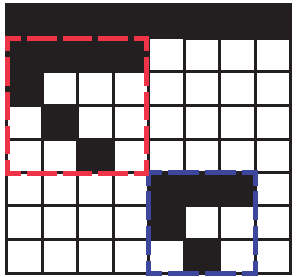
\includegraphics{figures/decompBigger.pdf}
	\caption{The inequality system in the figure can be divided into a transverse part and two local parts, namely the system enclosed within the red square and the system enclosed within the blue square. Each of the two subsystems can in themselves be solved using a decomposition into a transverse part and local parts.}
	\label{fig:decompBigger}
\end{figure}

We notice that it is up to the solver of the problem to identify the various local parts to best make use of the structure of the given problem.
However, it might be possible, also at a syntactical level, to identify potential useful partitions of the (in)equalities. This identification process is, though, left to future research. 

%\subsubsection*{\red{To be put somewhere (maybe)}}
%\red{Eliminating variables from the $X_i$ in the system consisting of all the produced constraints (and then the $z^k_{c,i}$s) will (probably) result in the same contraints being added (and being removed because of redundancy) as eliminating the $X_i$ variables from each of the smaller subproblem themselves, combining the constraints, and then eliminate the $z_i^k$-variables. The subproblems are smaller in size, so even if the two approaches adds and removes the same constraints, the latter is faster, and it is easier to keep track of which inequalities that are necessary to be taken into consideration when testing (other) inequalities for redundancy.}
%
%\red{For each defined variable $z^k_{c,i}$ there is by construction only two constraints containing it, and they would therefore be obvious choices for elimination. Though, starting with eliminating these is rather futile as we will just end with what we started with, and we could not exploit the division into subproblems.
%Hence, we solve each subproblem on its own \emph{keeping the variables} connecting them to the transverse constraints.} 

\section{Stowage capacity case study}\label{sec:results}
\subsection{Stowage model}
In this section we present the stowage model that is the point of origin for our projected capacity model. In other words, this model describes the (in)equality system which we want to project. The model is adapted from the PhD thesis of Delgado \cite{AlbertosThesis}; other models for stowage planning using actual vessel profiles can be found in e.g. \cite{DariosThesis}, \cite{pacino11} and \cite{pacino12}. We will not go into details of the model in this report, but will only present the essentials; the reader is referred to \cite{AlbertosThesis} %and \cite{pacino12} 
for further details. 
%
%%%%%%%%%%%%%%%%%%%%%%%%%%%%%%%%%%%%%5 \cite{pacino12}-ish
\subsubsection*{Description}
As shown in Figure~\ref{fig:vessel}, the cargo space of a container vessel is divided into
sections called \textit{bays} that each are divided into a grid by stacks and tiers (Figure~\ref{fig:bay_a}). Each stack and tier constitute a \emph{cell} that consists of two \emph{slots}. 

\begin{figure*}[tbh]
  \centering
  $\qquad$
	\subfloat[]{\label{fig:vessel} 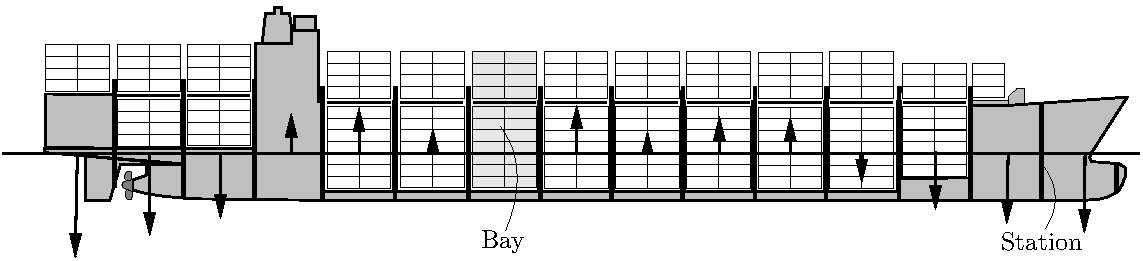
\includegraphics[scale=0.6]{figures/vessel1.pdf}}\\
  \subfloat[]{\label{fig:bay_a} 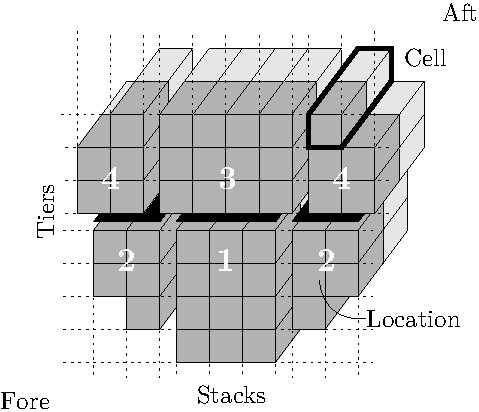
\includegraphics[scale=0.65]{figures/bay1.pdf}}~
	\qquad
%  \hfill
  \subfloat[]{\label{fig:bay_b}  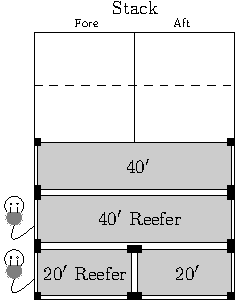
\includegraphics[scale=0.8]{figures/stack1.pdf}}~
  $\qquad$
\caption{(a) The arrangement of bays in a small container vessel. (b) A bay divided into cells given by stacks and tiers. The cells are grouped into four locations (c). A side view of a stack of containers with power plugs for reefer containers at bottom slots. {Adapted from \cite{AlbertosThesis}.}}
\label{fig:bay}
\end{figure*}

The containers transported on a vessel usually have a standard size that fits the cells and slots; the containers are normally (ISO standard) $8'$ wide, $8'6''$ high and $20'$,
$40'$ or $45'$ long, though we do not consider the latter in this report. Accordingly, a cell can hold either two $20'$ containers (one in each slot) or one $40'$ container (Figure~\ref{fig:bay_b}). Further, some containers are refrigerated (\emph{reefers}), and must be stowed at a power plug. 
The corners of the containers are constructed such that containers can be stacked, though $20'$ containers cannot
be stacked on top of $40'$ containers due to the lack of corner supports in th middle of $40'$ containers (see Figure~\ref{fig:bay_b}). 

The capacity of a container vessel is given in \emph{TEU} (Twenty-foot Equivalent Units), i.e. a standard $20'$ container as described above takes up one TEU, while a $40'$ container takes up two TEU. Each stack has a height and weight limit. Separate total weight limits for $20'$ and $40'$ containers exist, since only $20'$ containers rest on the middle support posts of the stack, while the end posts hold weight of $20'$ and $40'$ containers (Figure~\ref{fig:bay_b}). 

Though containers physically are placed in specific slots, the stowage models considered {specifies} how many containers of each \emph{type} should be placed in the subsections of each bay, called \emph{locations}. 
These locations emerge by dividing the bays {vertically} into sections on deck and below deck, respectively, and {horizontally} into a center section and symmetric side-sections, respectively; see Figure~\ref{fig:bay_a} which shows a bay divided into four location indicated by their number. The type of containers is here specified by the length, reefer-property and a weight class. The capacities for stacks translate to capacities for locations.

Besides the location-based capacity constraints, global hydrostatic constraints ensure the stability of the vessel. 
Stress forces arise as a result of gravitation acting downwards on the vessel and buoyancy acting upwards. Limits on these stress forces are given for a set of points along the vessel called \emph{frames}. %Figure~\ref{fig:vessel} shows the distribution of the vertical forces (resulting from gravitation and buoyancy) along the \red{sections/frames/bays} of the vessel. 
Buoyancy comes from the vessel's displacement of water and hence depends on the varying (and irregular) shape of the hull, which is given at a set of reference points called \emph{stations} (Figure~\ref{fig:stations}). At these stations, the area submerged in water can be approximated by linear functions of the vessel's displacement and longitudinal center of gravity (\emph{lcg}), and from this an approximation of the buoyancy force of the vessel between two consecutive stations can be calculated. 
Further hydrostatic constraints for ensuring the stability of the vessel is considered in \cite{AlbertosThesis} but is not considered here.
%
\begin{figure}[htbp]
  \centering
   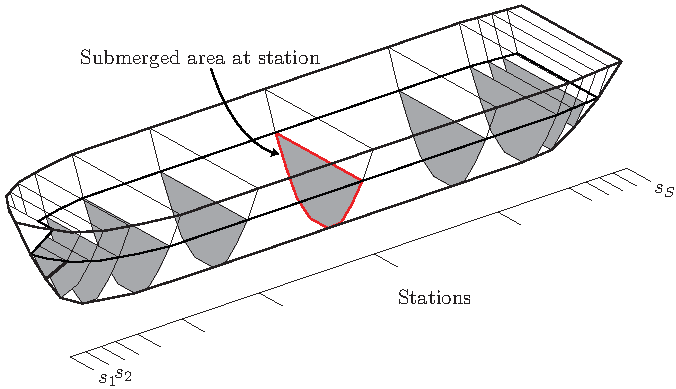
\includegraphics[scale=0.7]{figures/stations.pdf}
\caption{Stations of a vessel. Adapted from \cite{AlbertosThesis}.}
\label{fig:stations}
\end{figure}

Besides containers, vessels also carry ballast tanks in fixed positions along the vessel that can be filled with water. Doing this help handling the stability of the vessel so that otherwise unfeasible stowage configurations can be {achived}. {Bounds for these ballast tanks can be defined as well as an overall upper bound for these.}

\subsubsection*{Sets, variables, constants}
To formally describe the stacking and stability constraints of the considered stowage models, we use the sets, variables and constants summarized in Table~\ref{table:sets}, Table~\ref{table:vars} and Table~\ref{table:constants}, respectively.
\begin{table}[p]
\centering
\begin{tabular}{p{5cm}p{7.5cm}}%p{2cm}}
\multicolumn{2}{l}{\textbf{Sets}}\\
\hline\noalign{\smallskip}
$L$ 
	& Set of locations.\\
$\Sec$
	&Set of frames.\\
$\Sec^{\trt{f}},\Sec^\trt{a}\subseteq \Sec$
	&The frames \emph{fore} and \emph{aft}.\\
$S, S' = \{s_1,\ldots, s_S\}$ 
	&Number of stations and (ordered) set of stations.\\
$T$
	&Set of types of containers.\\ 
$T^\trt{20}$, $T^\trt{40}$, $T^\trt{R}$, $T^\trt{20R}$, $T^\trt{40R}\subseteq T$ 
	&Set of types that are $20'$ long, $40'$ long, reefers, $20'$ reefers, and $40'$ reefers, respectively.\\ 
$\mi{BT}$ 
	& Set of ballast tanks.\\
\end{tabular}
\caption{Sets used in the considered stowage models}
\label{table:sets}
\end{table}
%
\begin{table}[p]
\centering
\begin{tabular}{p{3.5cm}p{9cm}}
\multicolumn{2}{l}{\textbf{Decision variables}}\\
\hline
$x_{l,\tau}\in \mathbb{R}^+_0$
		&Number of containers of each type $\tau\in T$ to be stowed at each location $l\in L$.\\
$x_b\in \mathbb{R}^+_0$
		& The weight of each ballast tank $b\in \mi{BT}$.\\
\\
\multicolumn{2}{l}{\textbf{Auxilliary variables}}\\
\hline
$\weight_l\in \mathbb{R}^+_0$
		&The weight of all containers stowed at each location $l\in L$.\\
$x_\tau\in \mathbb{R}^+_0$
		&The total number of containers of each type $\tau\in T$.\\
$\shear_f\in \mathbb{R}$
		&{The shear force at each frame $f\in \Sec$}.\\
$lcg\in\mathbb{R}$
		&{The longitudinal center of gravity}.\\
$\bonjean_s \in\mathbb{R}$
		&{The buoyancy force at each section between $s\in S'\setminus\{s_S\}$ and the next station.}\\
$\shear_f^{\trt{c},e}$, $\shear_f^{\trt{bt},e}$, $\shear_f^{\trt{bc},e}\in\mathbb{R}$
		&The contribution to the shear force for/aft (${e}\in\{\trt{f},\trt{a}\}$) each frame $f\in\Sec$ from containers (\trt{c})/ballast tanks (\trt{bt})/buoyancy (\trt{bc})
\end{tabular}
\caption{Variables used in the considered stowage models}\label{table:vars}
\end{table}
Regarding the variables, we note that even though $x_{l,\tau}$ is a number of containers and hence a natural number, we model it as a reel number to ensure that the resulting model is an LP. \red{This approximation is fine, since...} 
%
\begin{table}[p]
\centering
\begin{tabular}{p{4.5cm}p{8cm}}%p{2cm}}
\multicolumn{2}{l}{\textbf{Constants}}\\
\hline\noalign{\smallskip}
$\Ca_l^\trt{20}$, $\Ca_l^\trt{40}$, $\Ca_l^\trt{TEU}$, $\Ca_l^\trt{RS}$, $\Ca_l^\trt{RC}$, 
$\Ca_l^\trt{W20}$, $\Ca_l^\trt{W40}$
		& The capacity for each location $l\in L$, w.r.t. $20'$ containers, $40'$ container, TEU, reefer slots, reefer cells, weight of $20'$ containers, and weight of $40'$ containers, respectively.\\
%\hline
$\Weight_\tau$
		&The weight of a type of container $\tau\in T$.\\
%\hline
$\Bonj^\trt{lcg}_s$, $\Bonj^\trt{W}_s$
		&{Coefficients for the linearization of the submerged area at each station $s\in S'$.}\\
%\hline
$D_s$ &
		The distance between $s\in S'\setminus\{s_S\}$ and the next station.\\
%\hline
$W^\trt{f}_f$, $W^\trt{a}_f$
		&{The constant weight of the vessel fore/aft each frame $f\in\Sec$ (light ship)}\\
%\hline
$\Prop^{e}_{f,l}$, $\Prop^{e}_{f,b}$, $\Prop^{e}_{f,s}\in [0,1]$
		& The fraction of each location $l\in L$/ballast tank $b\in \mi{BT}$/section between $s\in S'\setminus\{s_S\}$ and the next station that lies fore/aft (${e}\in\{\trt{f},\trt{a}\}$) each frame $f\in\Sec$.\\
%\hline
$\mi{UB}(\mi{lcg})$, $\mi{lb}(\mi{lcg})$,\newline $\mi{UB}(\mi{sf}_f)$, $\mi{lb}(\mi{sf}_f)$,\newline 
 $\mi{UB}(x_b)$, $\mi{UB}(\trt{WBT})$,\newline $\mi{lb}(\trt{WBT})$
		&The upper and lower bounds for the lcg, shear force at each frame $f\in \Sec$, the weight for each ballast tank $b\in BT$ (upper bound only), plus 
		the weight of ballast tanks in total, respectively.\\
\end{tabular}
\caption{Constants used in the considered stowage models}\label{table:constants}
\end{table}
%
\subsubsection*{Constraints}
\paragraph{Location-based capacity constraints}
Firstly, we have constraints that ensure that for each location of the vessel, the stowed containers are within the allowed capacities w.r.t. the number of $20'$ containers, $40'$ containers, TEUs, and the weight of the $20'$ and $40'$ containers, respectively. These constraint are modeled in the inequalities \eqref{20Cap}-\eqref{weight40Cap} below.
{Likewise, we have a constraint, \eqref{combinedWeightCap}, that ensures that the weight of a location is within limits, taken the different distribution of the weight of $40'$ containers, respectively $20'$ containers, within a slot into consideration; the weight of a $40'$ container is distributed on the four outer corner places of a slot while the weight of $20'$ containers also rest on the inner corners of the slot.}
Lastly, \eqref{reeferSlotCap} and \eqref{reeferCellCap} ensure that each reefer container can be refrigerated, and that {the total number of cells taken up by the reefer containers are within capacity}, respectively. 
\begin{align}
{\forall l \in L:}&\quad
	%\tag{20'' capacity}
	\label{20Cap}
	{\sum_{\tau \in T^\trt{20}} x_{l,\tau} \leq \Ca_l^\trt{20}}\\
%
%\tag{40'' capacity}
\label{40Cap}    	
	{\forall l \in L:}&\quad
	{\sum_{\tau \in T^\trt{40}} 2\cdot x_{l,\tau} \leq \Ca_l^\trt{40}}\\
%
%\tag{TEU capacity}
\label{teuCap}
	\forall l \in L:&\quad
	\sum_{\tau \in T^\trt{20}} x_{l,\tau} + 2\cdot\sum_{\tau \in T^\trt{40}} x_{l,\tau} \leq \Ca_l^\trt{TEU}\\
%
%\tag{Volume capacity}
%\label{volCap}
%\red{\forall l \in L:&\quad\sum_{\tau \in T} \Vol_\tau\cdot x_{l,\tau} \leq \Ca_l^\trt{vol}}\\
%
%Weight vars and weight capacity
%\tag{20'' weight capacity}
\label{weight20Cap}
	\forall l \in L:&\quad\sum_{\tau \in T^\trt{20}} \Weight_\tau\cdot x_{l,\tau} \leq \Ca_l^\trt{W20}\\
%
%\tag{40'' weight capacity}
\label{weight40Cap}
	\forall l \in L:&\quad\sum_{\tau \in T^\trt{40}} \Weight_\tau\cdot x_{l,\tau} \leq \Ca_l^\trt{W40}\\
%
%\tag{Combined weight capacity}
\label{combinedWeightCap}
	\forall l \in L:&\quad 0.5\cdot \sum_{\tau \in T^\trt{20}} \Weight_\tau\cdot x_{l,\tau} + \sum_{\tau \in T^\trt{40}		} \Weight_\tau\cdot x_{l,\tau} \leq \Ca_l^\trt{W40}\\
%
%	//Reeer constraint
%\tag{Reefer slot capacity}
\label{reeferSlotCap}
	\forall l \in L:&\quad\sum_{\tau \in T^\trt{R}} x_{l,\tau} \leq \Ca_l^\trt{RS}\\
%
%\tag{Reefer cell capacity}
\label{reeferCellCap}
	{\forall l \in L:}&\quad
	{\sum_{\tau \in T^\trt{20R}} 0.5\cdot x_{l,\tau} + \sum_{\tau \in T^\trt{40R}} x_{l,\tau} \leq \Ca_l^\trt{RC}}
%   	
%//Type capacity constraint
%\label{typesConstraints}
%\red{\forall l \in L, \tau \in T:}&\quad
%\red{\sum_{\tau' \in TypesConstraint_\tau} x_{l,\tau'} \leq LocationsTypesCap_{l,\tau}}\\
\end{align}	 
%
\paragraph{Defined variables and bounds}
The constraint in \eqref{typeDef} defines the variables, $x_\tau$, that specifies how many containers of a specific type $\tau$ is stowed on the vessel. These are the variables that we want the projected (in)equality system to be expressed in.
\begin{equation}
\label{typeDef}%\tag{Type definition}
	\forall{\tau \in T}: x_\tau = \sum_{l\in L} x_{l,\tau}
\end{equation}
\eqref{totalWeightDef} below defines the total weight of the containers stowed in each location, since this number is used in further calculations of the hydrostatic constraints (see further below). 
\begin{equation}
%\tag{Total weight definition}
\label{totalWeightDef}
	\forall l \in L:\quad \weight_l = \sum_{\tau \in T} \Weight_\tau\cdot x_{l,\tau}\\
\end{equation}
We also ensure that the number of containers placed at each location of each type as well as the amount of ballast in the ballast tanks is positive. %The positivity of $\weight_l$ and $x_\tau$ follows from these bounds, so we do not need to include those\marginpar{or should I?}.
%\begin{align}
%\label{btPos}
%	\forall b\in BT:&\quad x_{b}\geq 0.
%\label{wPos}
%	\forall l\in L:& w_{l}\geq 0.\\
%\label{typePos}
%	\forall l\in L, \tau\in T:& x_{l,\tau}\geq 0.\\
%\end{align}
For the ballast tanks, we also require that each tank's content is within limits, as well as the total content. These constraints are given in \eqref{btLim} and \eqref{BTLim} below.
\begin{align}
\label{xPos}
	\forall l\in L, \tau\in T:&\quad x_{l,\tau}\geq 0.\\
%\tag{Limits for each tank}
\label{btLim}
	\forall b \in BT:	&\quad 0 \leq x_b \leq \mi{UB}(x_b)\\ 
%
%\tag{Limits for total weight of tanks}
\label{BTLim}
	\mi{lb}(\trt{WBT}) &\leq \sum_{b \in BT} x_b	\leq \mi{UB}(\trt{WBT})
\end{align}
%
\paragraph{Hydrostatic constraints}
%For vessel stability, the model in \cite{AlbertosThesis} uses variable displacement, and for this it uses discrete displacement intervals.  
%To avoid integer variables we consider here a constant displacement interval, \red{and we assume that the stowed containers lie within $75$ to $85$ percent of the vessel's maximal allowable displacement.} \marginpar{maybe put in model}
At each station the submerged area of the cross-section has been linearized as a function of the lcg, and the buoyancy force for each section between consecutive stations are calculated as the average of the two areas times the distance between the two stations \eqref{bonjeanVarDef}. 
Instead of calculating the vessel's lcg, we only require it to be within a given interval \eqref{lcgLim}.
%For each bonjean station $s$ (except the last) %\red{(well, it is measured in between two stations and the assigned to the first station)}, 
%a bonjean variable is defined as the average \red{of something ... of the station $s$ and the next station, that is, the variable defines the averaged force in the middle between the two stations}.

The shear forces at each frame can then be calculated as the sum of the constant weight of the vessel fore (aft) the frame, the weight of the containers and ballast tanks for (aft) the frame, and the buoyancy fore (aft) the frame, the latter of which which will be negative, see \eqref{eq:shear}. For each of the frames, we then require these shear forces to be within limits \eqref{shearLimits}.   
\begin{gather}
\forall s_i \in S'\setminus\{s_S\}:\;
\bonjean_{s_i} = \frac{1}{2}\cdot D_{s_i}\cdot(\Bonj^\trt{W}_{s_i} + \mi{lcg}\cdot \Bonj^\trt{lcg}_{s_i}	+ \Bonj^\trt{W}_{s_{i+1}} + \mi{lcg}\cdot \Bonj^\trt{lcg}_{s_{i+1}})
\label{bonjeanVarDef}\\
%
\mi{lb}(\mi{lcg}) \leq \mi{lcg} \leq \mi{UB}(\mi{lcg})
\label{lcgLim}\\
%
\forall {e}\in\{\trt{f},\trt{a}\}, f \in \Sec^{e}:\;
\shear_f = W^{e}_f+ \sum_{l\in L} \weight_l\cdot \Prop_{f,l}^{e} + \sum_{b \in BT} x_b\cdot \Prop^{e}_{f,b} 	+ \smashoperator{\sum_{s_i \in S'\setminus\{s_S\}}}\bonjean_{s_i}\cdot \Prop^{e}_{f,s_i}
\label{eq:shear}\\
%
\forall f \in \Sec:\;	\mi{lb}(\shear_f)\leq	\shear_f \leq \mi{UB}(\shear_f)
\label{shearLimits}
\end{gather}
%
\subsection{Test results}\label{sec:testResults}
To do a nested decomposition (see section \ref{sec:nested}), we will, though, divide the constraints in \eqref{eq:shear} in a part coming from the containers, ballast tanks and bouyancy, respectively, using auxiliary variables. Thus \eqref{eq:shear} is replaced with \eqref{shearLocDef}-\eqref{shearDef} below.
\begin{align}
\label{shearLocDef} 
\forall {e}\in\{\trt{f},\trt{a}\}, f \in \Sec^{e}:&\;
	\shear^{\trt{c},e}_f = \sum_{l \in L} \weight_l\cdot \Prop^{e}_{f,l}\\
%
\forall {e}\in\{\trt{f},\trt{a}\}, f \in \Sec^{e}:&\;
	\label{shearTanksDef}
	\shear^{\trt{bt},e}_f = \sum_{b \in \mi{BT}} x_b\cdot \Prop^{e}_{f,b} \\		
%
\forall {e}\in\{\trt{f},\trt{a}\}, f \in \Sec^{e}:&\;
	\label{shearBonjDef}
	\shear^{\trt{bc},e}_f = \sum_{s_i \in S'\setminus\{s_S\}} \bonjean_{s_i}\cdot \Prop^{e}_{f,s_i} \\
%
\forall {e}\in\{\trt{f},\trt{a}\}, f \in \Sec^\trt{e}:&\;
	\label{shearDef}
 	\shear_f = W^{e}_f +	\shear^{\trt{c},e}_f+ \shear^{\trt{bt},e}_f + \shear^{\trt{bc},e}_f
\end{align}
%
%
We have tested our methods on three different models, each including a different number of the constraints presented in the previous section and above. In all cases, we wanted a model capturing all the dependencies between the  variables $x_\tau$, and only those. Hence we project the variables $\VAR(S)\setminus \set{x_\tau}{\tau\in T}$ where $S$ is the system consisting of the (in)equalities corresponding to the constraints of the model.

We have used data from our industrial partner, Maersk, from a vessel with a capacity of $15.500$ TEU, $91$ locations, $27$ ballast tanks and $33$ stations. There are $25$ frame points, however, we have only used one fore and one aft (in the two models considering hydrostatics). In all models, we considered 12 types, $T = \{20', 40'\}\times \{6t, 21t, 27t\}\times\{\trt{R}, \trt{NR}\}$, that are defined according to the length, the weight class and the reefer property of the containers.

In the two tables below we show which (in)equalities are present in the 3 (in)equality systems $S_1$, $S_2$ and $S_3$ that have been tested, and we state the size of each model given in number of (in)equalities, number of variables and the two numbers multiplied. Similarly we present the size of the projected (in)equality systems together with the approximate time taken to obtain those projections. 

The (in)equality system $S_1$ includes $3$ capacity constraints per location and shear force calculations at $2$ frame points; $S_2$ includes all capacity constraints for each location but no calculations of shear forces. $S_3$ includes 6 capacity constraints per location and shear force calculations at the two frames.
\begin{table}[H]
\centering
{\renewcommand{\arraystretch}{1.2}
\begin{tabular}[t]{l|p{9cm}}
%\hline
(In)eq. system&Constraints included\\
\hline
$S_1$& \eqref{teuCap}, \eqref{combinedWeightCap}, \eqref{reeferCellCap}, \eqref{typeDef}, \eqref{totalWeightDef}, \eqref{xPos}, \eqref{btLim}, \eqref{BTLim}, \eqref{bonjeanVarDef},  \eqref{lcgLim}, \eqref{shearLimits}, {\eqref{shearLocDef}}, \eqref{shearTanksDef}, \eqref{shearBonjDef}, \eqref{shearDef}\\
\hline
$S_2$&\eqref{20Cap}, \eqref{40Cap}, \eqref{teuCap}, \eqref{weight20Cap}, \eqref{weight40Cap}, \eqref{combinedWeightCap}, \eqref{reeferSlotCap}, \eqref{reeferCellCap}, \eqref{typeDef}, \eqref{totalWeightDef}, \eqref{xPos}\\
\hline
$S_3$& \eqref{20Cap}, \eqref{40Cap}, \eqref{teuCap}, \eqref{combinedWeightCap}, \eqref{reeferSlotCap}, \eqref{reeferCellCap},  \eqref{typeDef}, \eqref{totalWeightDef}, \eqref{xPos}, \eqref{btLim}, \eqref{BTLim}, \eqref{bonjeanVarDef}, \eqref{lcgLim}, \eqref{shearLimits}, {\eqref{shearLocDef}}, \eqref{shearTanksDef}, \eqref{shearBonjDef},  \eqref{shearDef}\\
%\hline
\end{tabular}
}
\caption{Constraints included in test systems.}\label{fig:constraints}
\end{table}
%

The test have been done on a laptop with an Intel$^\text{\textregistered}$ Core\texttrademark\; i7-4600U-processor with a frequency of 2.10-3.3 GHz, 8GB RAM, and with 2 cores and 4 threads. The computer has also been used to perform other tasks while doing the projection, and 3 threads were used to run the parallel redundancy checks. The time used to make the projection is therefore not accurate, but still gives an indication of the running time (especially when these are compared across the test results). 
%
%%%%GOOD UNTIL HERE
\begin{table}[H]
\centering
\noindent\begin{tabular}{|l|r|r|r|r|r|r|r|}
\hline
(In)equality&App. time&\multicolumn{3}{c|}{Size of system}&\multicolumn{3}{c|}{Size of projected system}\\ %Size doesn't include bounds
system&&{\#(in)eqs}&{\#vars}&${\#\text{ineqs}\cdot\#\text{vars}}$&{\#(in)eqs}&{\#vars}&${\#\text{ineqs}\cdot\#\text{vars}}$\\
%\scriptsize{\#vars}&$\substack{\#\text{ineqs}\quad\\\cdot\#\text{vars}}$\\
\hline
$S_1$&6 m&537&1092&586,404&26&12&312\\
$S_2$&18.5 h&922&1209&1,114,698&42&12&504\\
$S_3$&97 h&811&1171&949,681&106&12&1272\\
\hline
\end{tabular}
\caption{Sizes of original and projected systems.}\label{tab:results}
\end{table}
%


In all three test cases, the system consisting of the (in)equalities using $x_{l,\tau}$ and $\weight_l$ were set aside; this is the system corresponding to the constraints \eqref{20Cap}-\eqref{xPos} (for $S_2$) plus \eqref{shearLocDef} (for $S_1$ and $S_3$). Then these systems were decomposed according to the locations, and the variables $x_{l,\tau}$ and $\weight_l$ were eliminated, leaving a system over $x_\tau$ (for $S_1$), or $x_\tau$ and $\shear^{\trt{c},e}_f$ (for $S_1$ and $S_3$). The decomposition was done such that $X_i = \set{x_{l,\tau}}{\tau \in T, l\in P^0_i}\cup\set{\weight_l}{l\in P^0_i}$ for each $1\leq i \leq 45$, where  
\begin{align*}
(P^0_1,P^0_2,\ldots, P^0_{45}) =
&\big(\{0,1,2\}, \{3,4\}, \{5,6\}, \{7,8\}, \{9,10\}, \{11,12\}, \{13,14\}, \{15,16\}, \{17,18\}, \\
&\{19,20\}, \{21,22\},\{23,24\}, \{25,26\}, \{27,28\}, \{29,30\}, \{31,32\}, \{33,34\}, \\
&\{35,36\}, \{37,38\}, \{39,40\}, \{41,42\}, \{43,44\}, \{45,46\}, \{47,48\}, \{49,50\}, \\
&\{51,52\}, \{53,54\}, \{55,56\}, \{57,58\}, \{59,60\}, \{61,62\}, \{63,64\}, \{65,66\}, \\
&\{67,68\}, \{69,70\}, \{71,72\}, \{73,74\}, \{75,76\}, \{77,78\}, \{79,80\}, \{81,82\}, \\
&\{83,84\}, \{85,86\}, \{87,88\}, \{89,90\}, \{91\}\big).
\end{align*}
For $S_1$ and $S_3$, the list of partitions $\mathfrak{P}$ was $\mathfrak{P} = (\mathbb{P}^1, \mathbb{P}^2, \mathbb{P}^3, \mathbb{P}^4, \mathbb{P}^5)$, where 
\begin{align*}
\mathbb{P}^1 &= \big( \{0,1\}, \{2,3\}, \{4,5\}, \{6,7\}, \{8,9\}, \{10,11\}, \{12,13\}, \{14,15\}, \{16,17\},\\
						 & \quad \{18,19\}, \{20,21\}, \{22,23\}, \{24,25\}, \{26,27\}, \{28,29\}, \{30,31\}, \{32,33\},\\
						 & \quad \{34,35\}, \{36,37\}, \{38,39\}, \{40,41\}, \{42,43\}, \{44,45\} \big),\\
\mathbb{P}^2 &= \big( \{0,1\}, \{2,3\}, \{4,5\}, \{6,7\}, \{8,9\}, \{10,11\}, \{12,13\}, \{14,15\}, \{16,17\},\\
						 & \quad \{18,19\}, \{20,21\}, \{22\} \big),\\
\mathbb{P}^3 &= \big( \{0,1\}, \{2,3\}, \{4,5\}, \{6,7\}, \{8,9\}, \{10,11\} \big),\\
\mathbb{P}^4 &= \big( \{0,1\}, \{2,3\}, \{4,5\} \big),\\
\mathbb{P}^5 &= \big(\{0\}, \{1,2\} \big).
\end{align*}
%
For $S_2$, the partitions where $\mathfrak{P}' = (\mathbb{P}'^1, \mathbb{P}'^2, \mathbb{P}'^3, \mathbb{P}'^4, \mathbb{P}'^5)$, where 
\begin{align*}
\mathbb{P}'^1 &= \mathbb{P}'^1,\\  
\mathbb{P}'^2 &= \big\{ \{0,1\}, \{2,3\}, \{4,5\}, \{6,16\}, \{8,9\}, \{10,18\}, \{12,13\}, \{14,15\}, \{7,17\},
						   \{11,19\},\\& \{20,21\}, \{22\} \big\},\\
\mathbb{P}'^3 &= \big\{ \{0,2\}, \{1,3\}, \{4,6\}, \{5,7\}, \{8,10\}, \{9,11\} \big\},\\
\mathbb{P}'^4 &= \big\{ \{0,1\}, \{2,4\}, \{3,5\} \big\},\\
\mathbb{P}'^5 & = \mathbb{P}^5.
\end{align*}

The reason for having $\mathfrak{P}'$ like this (and not just ``numerical'') was to ``pair'' partitions according to the size of the produced (sub)projections such that some of the smaller projections were paired with some of the larger projection. The reason that some of the (sub)projections were smaller is partly that some of the locations have no reefer capacity, so $x_{l,\tau}$ for such a location and a $\tau$ that is a reefer type is quickly set to $0$, which makes the projection smaller.

For $S_2$, making the above projection resulted in the required system expressed only in the $x_\tau$-variables.

For both $S_1$ and $S_3$ we projected yet two more subsystems; the subsystem consisting of the (in)equalities relating to buoyancy (\eqref{bonjeanVarDef}, \eqref{lcgLim}  and \eqref{shearBonjDef}) were projected w.r.t. $lcg$ and $\bonjean_s$ (leaving only the $\shear^{\trt{bc,f}}_f$ and $\shear^{\trt{bc,a}}_f$ variables), while the subsystem relating to ballast tanks (\eqref{btLim}, \eqref{BTLim} and \eqref{shearTanksDef}) were projected w.r.t. $x_b$ (leaving the $\shear^\trt{bt,f}_f$ and $\shear^\trt{bt,a}_f$ variables). 
For both $S_1$ and $S_3$, the three projected subsystems were then joined together with the (in)equalities \eqref{shearLimits} and \eqref{shearDef}, relating to the shear force. In this final system, we then eliminated the $\shear^{\trt{c},e}_f$, $\shear^{\trt{bt},e}_f$, $\shear^{\trt{bc},e}_f$, and the $\shear_f$-variables, which resulted in a system over the $x_\tau$-variables as required. %\marginpar{Actually, we had the \eqref{shearLocDef} included in the ``container''-part, but I am not sure if this makes a difference}

\begin{figure}[p]
	\centering
		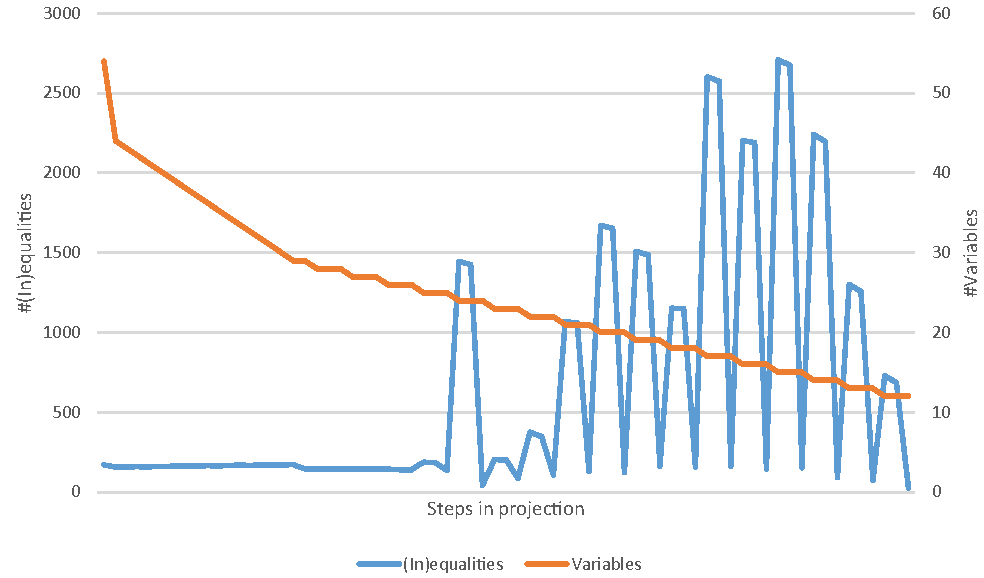
\includegraphics[scale=0.6]{figures/FinalProjection-29-2Shear.pdf}
	\caption{Projection of the final system stemming from $S_1$. }
	\label{fig:FinalProjectionS1}
\end{figure}

\begin{figure}[p]
	\centering
		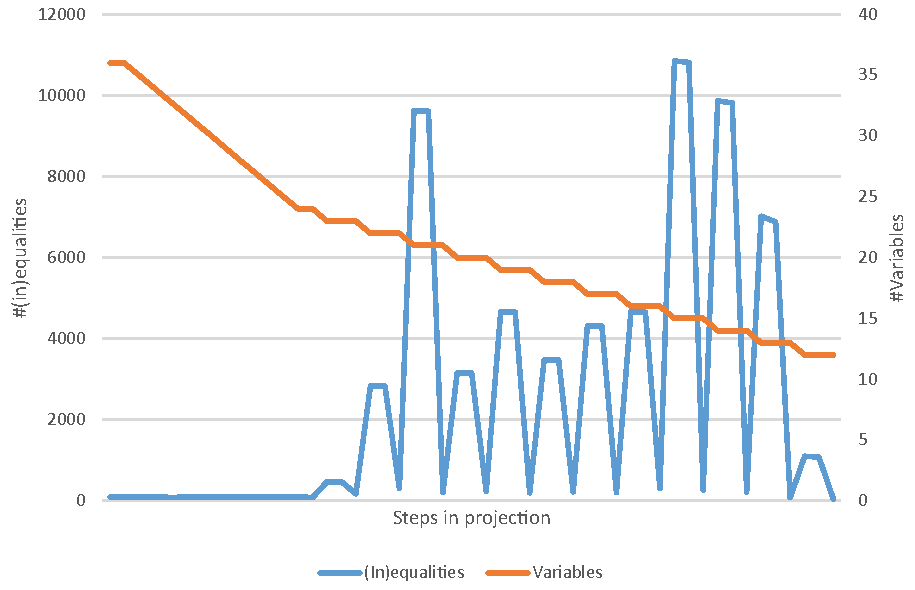
\includegraphics[scale=0.6]{figures/FinalProjection-24.pdf}
	\caption{Projection of the final system stemming from $S_2$. }
	\label{fig:FinalProjectionS2}
\end{figure}

\begin{figure}[p]
	\centering
		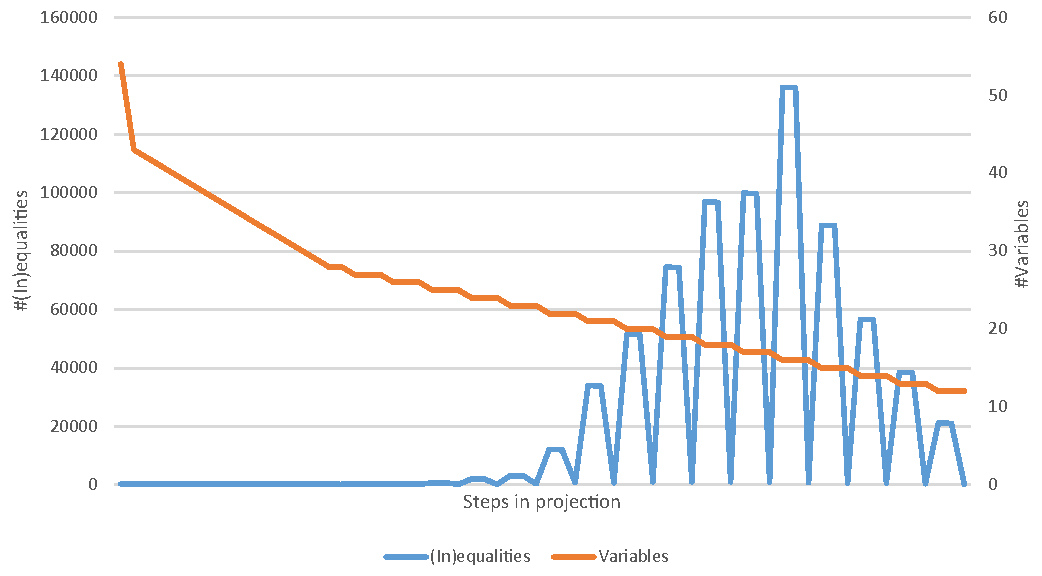
\includegraphics[scale=0.6]{figures/FinalProjection-30.pdf}
	\caption{Projection of the final system stemming from $S_3$. }
	\label{fig:FinalProjectionS3}
\end{figure}

To give the reader an idea of the how the number of (in)equalities and variables, respectively progress, Figure~\ref{fig:FinalProjectionS1}, Figure~\ref{fig:FinalProjectionS2} and Figure~\ref{fig:FinalProjectionS3} show the evolution of these numbers when projecting the mentioned final system stemming from $S_3$, which is the system producing the largest intermediary systems. Each ``step'' in these graphs corresponds to either the preprocessing or ''clean-up'' (as a whole), Gauss-elimination of one variable, FM-elimination of one variable, or a complete redundancy removal of the system. The first part where the number of (in)equalities is reasonable stable (when seen in this scale) corresponds to the preprocessing and Gauss-elimination part. 
This is followed by repeated steps of FM-elimination (the ``peaks'' in the number of (in)equalities), clean-up (the ``flat'' part after the peaks) and redundancy removal (the ``valleys'').

We note that $S_3$ is the most time-consuming system to project of the three, and the final system as shown in Figure~\ref{fig:FinalProjectionS3} is by far the system (of all the subsystems that are projected) that produced the biggest intermediary systems.  

\subsection{Implementation notes}
{In our implementation of the program we use rationals for the coefficients and right-hand-sides}.

$\epsilon$ in Section~\ref{sec:uncertainty} is set to $0.01$, $\epsilon' = 0.000001$, and $\mathcal{K} = 10^{14}$. The optimization software CPLEX from IBM was used as lp-solver. 

{It should be noted, that because we use the almost redundant criteria when doing (sequential) redundancy, the system $S'$ returned by \Call{RemoveRedundancy}{} in line~\ref{ln:projx} of Algorithm~\ref{alg:project} is no longer completely identical to $\proj_x(S)$; $S'$ will most likely be an overapproximation of the projection. However, as previously mentioned, the parameters of a problem -- and this indeed holds for the particular problem we have considered -- are not necessarily very accurate, and small discrepancies between the returned projection and the actual projection is acceptable. It still remains to be shown that the overapproximation is not ``too big'' according to a given criterion.}
\\
\\
The program was implemented in Java.

In the implementation, we have used a list, not a set, for representing the (in)equalities in a system. Thus, at a given point, the (in)equality system $S$ might contain two (in)equalities $c$ and $c'$ for which $\vea(c)=\vea(c')$. However, either $c$ or $c'$ will be removed in the preprocessing/clean up step (when removing linearly dependent (in)equalities), and this does not influence the correctness of the algorithm(s).

We also normalize the (in)equalities in the inequality system such that the smallest absolute value of the coefficients is $1$. This also makes it easier to detect linear dependencies. 
\\
\\
We want to point out here, that the implemented program is non-deterministic due to a number of factors. 

Firstly, the almost redundant-criteria for removing inequalities in the sequential redundancy removal means that the order in which the inequalities are checked, matters. 
For two runs (on the same input system) to result in the exact  same projection, the variables must be projected in the same order, and at each variable elimination, the produced inequalities must be added in the same order (or checked for redundancy in the same order), and the redundancy check using CPLEX must result in the same yes/no answer (and $\kappa$-value). %This is in principle possible to achieve by having fixed orders of variables e.t.c. and setting some properties for CPLEX}.
 
Making use of parallel redundancy check means that when an inequality from a system is checked for redundancy in two different runs, another inequality might have been deemed redundant by another checker and hence have been removed in one run, while it is not in the other run (because the checker finished later). This can influence how long the check of the current inequality takes and influence the $\kappa$-value, so this effect can propagate. In the end, this might cause the set of removed (in)equalities to vary in the two runs altogether (because some inequalities in reality are redundant but cannot be determined to be so). 

Likewise, we make use of an in-build mechanism in Java for parallelism, namely streams. These are used for example when using the heuristic for finding out which variable should be removed. Again, this can of course be avoided.

In conclusion, with careful ordering of variables e.t.c., settings of parameters for CPLEX and avoidance of parallelism, non-determinism could possibly be avoided, but will most likely also be less efficient.  

\section{Related work and Discussion}\label{sec:related}
\paragraph{Original method and additions}
The presented, basic method for eliminating variables from a system of linear inequalities was first provided by Fourier in 1824 \cite{fourier2}, %\cite{fourier1}}, 
while Motzkin later reintroduced the method in his Ph.D. thesis \cite{motzkin}. \v{C}ernikov later augmented Fourier's algorithm with computational simple rules, which were later rediscovered by Kohler \cite{kohler67}, to both prevent additions of (some) redundant inequalities and remove others after construction \cite{chernikov63}, and used together with these rules, the presented method is also referred to as the Fourier-\v{C}ernikov method. 
These criteria-based rules rely on keeping track of an index set for each inequality $c\in S$, which contains (the index of) the inequalities from the original system that during the procedure have been combined to obtain $c$.   
However, though the proposed rules improve the method, they are incomplete,  i.e. they do not detect or remove all redundancies {(see e.g. \cite{imbert93} or \cite{lukatskii08}).

The method has subsequently been thoroughly studied, e.g. by Kohler \cite{kohler67}, Duffin \cite{duffin74} and Imbert \cite{imbert90}, \cite{imbert93}, and several additional rules were proposed in these papers to avoid the addition of redundant inequalities. 
Improving the run time of the procedure in various ways has also been studied, for example in \cite{huynh92} and in \cite{bastrakov15}, where a faster method is proposed to check the slower of the two \v{C}ernikov criteria. 

However, as with the rules of \v{C}ernikov and Kohler, the rules suggested by Duffin and Imbert do not identify and remove all redundant inequalities from an inequality system  and it is not clear to which extend applying these methods are compatible with removing every redundant inequality by solving a linear programming problem; the \v{C}ernikoc-rules are sound, but combining them with other sound redundancy removals (even such as removing duplicates) are in general unsound (\cite{jaffar93}, \cite{huynh92}, \cite{imbert93}, \cite{fouilhe}). \cite{imbert93} further states that he does not know ``a method which suppresses all redundancies, compatible with one of [the] Fourier elimination methods''. {However, \emph{strictly redundant} inequalities, whose corresponding hyperplane does not intersect the feasible area of the system
can be removed without compromising the soundness of the procedure with the additional rules {\cite{jaffar92}}. 

Furthermore, these rules for avoiding additions of unnecessary inequalities will not be correct when our ``almost redundant''-criteria is used for removing inequalities, and therefore we have chosen not to use the mentioned rules in our implementation. However, it would be possible to use them, without the added, full redundancy check, until the system e.g. reaches a certain size, at which it will then be fully reduced and the ``index sets'' reset, such that each inequality in this system is considered original.

%%%%%%%%%%%%%%%%%%%%%%%%%%%%%%%%%%%%%%%%%%%%%%%%%%%%%%%%%%%%%%%%%%%
\paragraph{Redundancy removal}
Separately, particularly within linear programming, work has also been done in the area of classifying and removing redundant inequalities in a inequality system as well as finding implicit equalities, e.g. \cite{telgen83}, \cite{lassez93}, \cite{karwan83}, \cite{andersen95}, \cite{mattheiss73} to name a few. 
Many of these (e.g. \cite{telgen83} and the {majority} of the methods presented in \cite{karwan83}) are to be performed within the simplex procedure (used to optimize an LP) or use the objective function and/or the optimal extreme point for the LP, and are hence not applicable for us. On the other hand, we have used cheap redundancy-identifications e.g. described in \cite{andersen95}, \cite{brearley75} and \cite{maros} in our preprocessing and clean-up method, as well as the removal of linearly dependent inequalities from \cite{lassez93}.

Although it would be an advantage to be able to identify implicit equalities (inequalities that must hold as equalities in the feasible area) such that they can be used in Gauss-elimination, a prior implementation suggested that not much was gained when trying to identify them, while the (na�ve) implementation was too time consuming.
However, it is not impossible, that our implementation could benefit from an implementation of more sophisticated methods for redundancy detection and removal instead of or in addition to (prior to) the reasonable straight-forward method applied here.  

%%%%%%%%%%%%%%%%%%%%%%%%%%%%%%%%%%%%%%%%%%%%%%%%%%%
\paragraph{Methods for projection not based on Fourier-Motzkin-elimination}
Other methods exist for computing the projection of a feasible area of an (in)equality system, that are not based on the method by Fourier and Motzkin. 

For example, in \cite{huynh92}, the authors describe a method (based on a method from \cite{lassez90}) that they recommend for dense systems, called the extreme point method. 
The method works by finding the extreme points of the polytope $P$ defined by the convex combinations of constraints in $S$ that eliminate the variables in $Y$. 
{Since the method finds extreme points and hence inequalities in the projection space incrementally, the method can be used to approximate the projection. The method is consequently used as a supplement to Fourier-Motzkin-elimination, Gauss elimination and full redundancy removal in \cite{simon05}, when the system being projected becomes too dense and an approximation is required.}

Huynh, Lassez and Lassez \cite{huynh92} further describe a method (based on \cite{lassezlassez}), the convex hull method, in which the projection of an inequality system $S$ is computed by successive refinements of an initial approximation of the projection. 
{According to the authors, the complexity of their algorithm ``depends essentially on the dimension of the projection of the output not the size of the input'' \cite{huynh92}}, and could therefore be an interesting alternative to Fourier-Motzkin-elimination in a case like the one we consider.

Another example is the method introduced in \cite{jones04}, called equality set projection, which computes all facets of the projection by first finding a random facet and then iteratively computing all adjacent facets (without revisiting them) {using a face-lattice}. 
This method is recommended by the authors for polytopes with a low facet count and a high vertex count.
 
Yet another approach to projection is presented in the work by \cite{jones08} %\red{\cite{howe12}} 
and \cite{fouilhe}. This work is based on parametric linear programming and the possibility to formulate a projection problem as a parametric programming problem. % \blue{(in more than one way)}. 
Hence techniques for finding the solution to the latter (e.g. a ``parametric'' version of simplex) can be used to find the projection. 
%%%\cite{jones08}:``Current projection methods that can operate in general dimensions can be grouped into four classes: Fourier elimination, block elimination, vertex enumeration and gift-wrapping approaches. Fourier-Motzkin elimination was originally described by Fourier in 1824 and can be thought of as the analogue of Gaussian elimination for linear %inequalities. Several versions and improvements to Fourier�s method have been proposed ([12, 13] to name a few), although the primary contribution was due to ? Cernikov [14] in 1963. In block elimination a polyhedron called the projection cone is defined whose extreme rays can then be used to find the defining halfspaces of the projection [15]. While there exist efficient methods for computing these extreme rays, (e.g. [16�18]), this approach may generate a large, and possibly exponential, number of redundant inequalities. It is also possible to enumerate the vertices of the polytope, compute their projection and then calculate the convex hull of the result. This approach can be efficient if there is a very small number of vertices, although it is possible that there may be an exponential number of vertices. The final approach enumerates the facets of the projection directly using a gift-wrapping approach [19, 20] and has been shown to be very efficient for a large class of polyhedra.''

It is an interesting direction for future research to see, if these methods are better than the currently used method for solving the problem described in this report, or whether they can be combined advantageously with our method. The described decomposition from Section~\ref{sec:decomp} could for example still be used while each of the subproblems could be projected using any method for projection. 

\paragraph{Fourier-Motzkin-based frameworks for projection}
In \cite{simon05} Simon and King combine Fourier-Motzkin-elimination, Gauss-elimination, removal of linearly dependent inequalities and complete redundancy removal in a similar fashion as we have done, to project sparse systems, and they use the extreme point method of Huynh \textit{et al.} \cite{huynh92} to make approximations of the projection when this is necessary. Their method is implemented as part of an argument-size analyzer for logic programs and tested on a variety of these. Their elimination procedure is therefore not applied once, but instead multiple times during an analysis, and their method and results are therefore hard to compare to ours. The (in)equality systems operated on are rather sparse and quite small, %(less than $30$ (in)equalities and less than $20$ variables).
while their objective is to do the analysis more efficiently (faster) than other methods (when using the polyhedral abstract domain for program analysis). %, and on the programs they analyze, they obtain run times mainly less than a few seconds.

Lukatskii and Shapot \cite{lukatskii08}, \cite{shapot12} describe and implement a projection method using Fourier-Motzkin-elimination augmented with \v{C}ernikov's rules. They further use a techniques for full redundancy removal examining the solution matrix for a basic solution. %\blue{(a solution, where at least $n$ out of $m$ inequalities are turned into equalities for a system with $n$ variables)}. 
Further they present and apply a method for ``additional matrix clean up'' where some almost redundant inequalities are removed. Their method for this is a little more elaborate than ours and involves a successive increase of the allowable deviation (corresponding to our $\epsilon$) and a permissible maximal ratio between the number of inequalities in the current system compared to the original system. 
They perform tests on a prototype implementation, where the sized of the test ranges between $81$ inequalities and $40$ variables to $201$ inequalities and $100$ variables, i.e. the systems they project are much smaller than the ones we have considered; granted, their run time is of course also smaller than ours. 

It is shown in \cite{shapot12} that if the polyhedron is solid, then the projection algorithm is stable, while 
for a singular polyhedron, small perturbations can lead to significant changes in the projection. However, no precise definitions of solid or singular polyhedra or of a stable algorithm are given, and it is not apparent which elements (\v{C}ernikov rules, redundancy removal, additional matrix clean-up), the algorithm referred to in the proposition, contains. %I assume that stable means that the algorithm �avoids magnifying small errors'' and that a solid polyhedron is an affine translation of a full-dimensional subspace while a singular polyhedron is not.] 
Given the examples shown in e.g. \cite{jaffar93}, that \v{C}ernikov's rules together with other forms of redundancy removals are unsound in general, and since Lukatskii and Shapot exactly augment the Fourier-\v{C}ernikov method with a procedure for removing all redundant inequalities and further use ``additional matrix clean-up'' it is unclear to the authors of this report whether their presented method works in general, especially since this question is not raised or relevant references mentioned.

\section{Conclusion}\label{sec:conclusion}
In this report we have presented a framework for projecting large, block structured inequality systems. The method incorporates procedures for preprocessing (including removal of linearly dependent inequalities), Gauss-elimination, Fourier-Motzkin-elimination, parallel, full redundancy removal and {adjustment} of the edges of the projecting (i.e. an approximation) using sequential redundancy removal of ``almost redundant'' inequalities. Further, the method uses a {novel} decomposition of the input problem to exploit its block structure. 
This decomposition method is usable not only together with Fourier-Motzkin elimination but with any other projection method; just replace $\Call{Project}{S^l_i,Y}$ in line~\ref{line:project1} and line~\ref{line:project2} of the \Call{Solve}{}-algorithm in Algorithm~\ref{alg:solve} with any other method producing a projection of $S^l_i$ w.r.t. $Y$.

Further, we have applied the presented method to a problem within the domain of liner shipping as we have obtained capacity models of manageable size from much larger stowage models. The obtained models are small and use approximately 100 times fewer variables, yet provide a better representation of the inter-dependencies between the number of stowed containers of different types than the very simple capacity models that are currently used. 

The results indicate that even though Fourier-Motzkin elimination has a bad time and space complexity, which often deems it unfit for practical use, it is possible to amend it to obtain projections of large, realistic size problems. 
The execution time for the test cases is still high and impractical for repeated use in online algorithm, but for the purpose of projecting a model (inequality system) once to obtain another, smaller model, the method {seems} viable.

\subsection{Future work}
As already mentioned in Chapter~\ref{sec:related} there are several interesting directions for future work, including
\begin{itemize}
\item using better methods for finding and removing redundant inequalities; 
\item using criteria such as \v{C}ernikov's (if compatible) to avoid the addition of some of the redundant inequalities;
\item using other methods for approximating the projection, while naturally also evaluating if these are actually better;
\item possibly find and use a better evaluation of when an approximation or adjustment of the projection is necessary.
\end{itemize}

Since our decomposition-approach also works for other projection methods, it is also evident to investigate whether it can be an advantage to combine this decomposition with other, potentially more efficient methods for projection.

A particular approach that could be interesting to pursue in our case is to add \v{C}ernikov rules to the Fourier-Motzkin-procedure, and only look for (and remove) \emph{strictly} redundant inequalities in parallel after each elimination. This should be done for each subproblem, while a full redundancy removal and/or approximation of the projection should be done when subproblems are combined at the ``next level'' of the decomposition, at which point the index-set would also be reset. Instead of using the sequential redundancy check to approximate the projection by removing almost redundant inequalities, it would here be possible to implement another method, potentially the extreme point method or the convex hull method, both described in \cite{huynh92}. The approximation approach in \cite{shapot12} could also be considered, particularly using an increasing $\epsilon$-value and a measure relatiing to the size of the original problem to determine when approximations should be done and to what extend.   

Other interesting topics for further research includes developing better heuristics for choosing the order of the variables to be substituted and deleted, plus automatic detection of useful decompositions of a given problem.
\bibliography{bibfile}{}
\bibliographystyle{alpha}
\section*{Appendix}
\projection*
\begin{proof}
We start by showing item \ref{lm:1.1}. Thus assume that $\var(S_1)\cap\var(S_2) = \emptyset$. Order the variables such that $x\prec y$ for all $x\in X\setminus Y$ and $y\in Y$.

First assume that $\ve{r}\in \proj_Y\big(\feas(S_1\cup S_2)\big)$. Then there exists values for the variables in $Y$, $\ve{r}_Y$, such that $(\ve{r},\ve{r}_Y)\in\feas(S_1\cup S_2)$, i.e. for all $c\in S_1\cup S_2$ it holds that $(\ve{r},\ve{r}_Y)\in\feas(c)$. Hence $(\ve{r},\ve{r}_Y)\in\feas(S_1)$ and $(\ve{r},\ve{r}_Y)\in\feas(S_2)$, so $\ve{r}\in \proj_Y(\feas(S_1))$ and $\ve{r}\in \proj_Y(\feas(S_2))$. That is, $\ve{r}\in\proj_Y\big(\feas(S_1)\big)\cap \proj_Y\big(\feas(S_2)\big)$.

On the other hand, let $Y_1 = Y\cap \var(S_1)$, $Y_2 = Y\cap \var(S_2)$ and $Y_3 = Y\setminus (Y_1 \cup Y_2)$, so that $Y = Y_1\dot\cup Y_2 \dot\cup Y_3$. Order the variables such that %``$\xx\setminus Y \prec Y_1 \prec Y_2 \prec Y_3$''. 
$x\prec y_1$, $y_1\prec y_2$ and $y_2\prec y_3$ for all $x\in \xx\setminus Y$, $y_1\in Y_1$, $y_2\in Y_2$ and $y_3\in Y_3$. 
Assume that $\ve{r}\in\proj_Y\big(\feas(S_1)\big)\cap \proj_Y\big(\feas(S_2)\big)$. Then $\ve{r}\in\proj_Y(\feas(S_1))$ and $\ve{r}\in\proj_Y(\feas(S_2))$.  
Hence there exists values $\ve{u}_1$ and $\ve{v}_1$ for the variables in $Y_1$, values $\ve{u}_2$ and $\ve{v}_2$ for the variables in $Y_2$, and values $\ve{u}_3$ and $\ve{v}_3$ for the variables in $Y_3$ such that $\vea(c)\cdot (\ve{r}, \ve{u}_1, \ve{u}_2, \ve{u}_3)\odot_c \rhs(c)$ for all $c\in S_1$, and $\vea(c')\cdot (\ve{r}, \ve{v}_1, \ve{v}_2, \ve{v}_3)\odot_{c'} \rhs(c')$ for all $c'\in S_2$. 

Now consider the vector $(\ve{r}, \ve{u}_1, \ve{v}_2, \ve{0})$. Since $\coef(x,c)=0$ for all $x\in Y_2\cup Y_3$ and $c\in S_1$, we have that 
\begin{align*}
\vea(c)\cdot (\ve{r}, \ve{u}_1, \ve{v}_2, \ve{0}) 
&= \vea(c_{X\setminus Y})\cdot \ve{r} + \vea(c_{Y_1})\cdot \ve{u}_1 + \vea(c_{Y_2})\cdot \ve{v}_2 + \vea(c_{Y_3})\cdot\ve{0}\\ 
&= \vea(c_{X\setminus Y})\cdot \ve{r} + \vea(c_{Y_1})\cdot \ve{u}_1 + \ve{0}\cdot \ve{v}_2 + \ve{0}\cdot\ve{0}\\ 
&= \vea(c_{X\setminus Y})\cdot \ve{r} + \vea(c_{Y_1})\cdot \ve{u}_1 + \vea(c_{Y_2})\cdot \ve{u}_2 + \vea(c_{Y_3})\cdot \ve{u}_3\\
&= \vea(c)\cdot (\ve{r},\ve{u}_1,\ve{u}_2,\ve{u}_3) \odot_c \rhs(c)
\end{align*}
for all $c\in S_1$. Likewise
\begin{align*}
\vea(c')\cdot (\ve{r}, \ve{u}_1, \ve{v}_2, \ve{0}) 
&= \vea(c'_{X\setminus Y})\cdot \ve{r} + \vea(c'_{Y_1})\cdot \ve{u}_1 + \vea(c'_{Y_2})\cdot \ve{v}_2 + \vea(c'_{Y_3})\cdot\ve{0}\\ 
&= \vea(c'_{X\setminus Y})\cdot \ve{r} + \ve{0}\cdot \ve{u}_1 + \vea(c'_{Y_2})\cdot \ve{v}_2 + \ve{0}\cdot\ve{0}\\ 
&= \vea(c'_{X\setminus Y})\cdot \ve{r} + \vea(c'_{Y_1})\cdot \ve{v}_1 + \vea(c'_{Y_2})\cdot \ve{v}_2 + \vea(c'_{Y_3})\cdot \ve{v}_3\\
&= \vea(c')\cdot (\ve{r},\ve{v}_1,\ve{v}_2,\ve{v}_3) \odot_{c'} \rhs(c')
\end{align*}
for all $c'\in S_2$.
That is, there exists an $\ve{r}_Y$, namely $(\ve{u}_1,\ve{v}_2,\ve{0})$, such that $(\ve{r},\ve{r}_Y)\in\feas(S_1 \cup S_2)$, i.e. $\ve{r}\in \proj_Y(\feas(S_1\cup S_2))$.

This shows item \ref{lm:1.1} of the lemma.
\\\\
Now we will show item \ref{lm:1.2}. Thus assume that $\var(S_1)\cap Y = \emptyset$. Order the variables such that $x\prec y$ for all $x\in X\setminus Y$ and $y\in Y$.

First assume that $\ve{r}\in \feas\big((S_1)_{X\setminus Y}\big)\cap \proj_Y\big(\feas(S_2)\big)$. Then it holds that $\vea(c)_{X\setminus Y}\cdot\;\ve{r} \odot_c\rhs(c)$ for all $c\in S_1$, and there exists an $\ve{r}_Y$, denoting values for the variables in $Y$, such that $(\vea(c'_{X\setminus Y}),\vea(c'_Y))\cdot(\ve{r},\ve{r}_Y)\odot_{c'}\rhs(c')$ for all $c'\in S_2$.
Since $\var(S_1)\cap Y = \emptyset$, we have that $\vea(c_Y)=\ve{0}$ for all $c\in S_1$, and hence 
$\vea(c_{X\setminus Y})\cdot\ve{r} = \vea(c_{X\setminus Y})\cdot\ve{r} + \vea(c_Y)\cdot\ve{r}_Y = (\vea(c_{X\setminus Y}),\vea(c_Y))\cdot(\ve{r},\ve{r}_Y)\odot_{c}\rhs(c)$ for all $c\in S_1$. 

Thus $\ve{r}_Y$ is such that $(\vea(c_{X\setminus Y}),\vea(c_Y))\cdot(\ve{r},\ve{r}_Y)\odot_{c}\rhs(c)$ for all $c\in S_1\cup S_2$, i.e. there exists an $\ve{r}_Y$ such that $(\ve{r},\ve{r}_Y)\in \feas(S_1\cup S_2)$. That is, $\ve{r}\in \proj_Y\big(\feas(S_1\cup S_2)\big)$.

On the other hand, assume that $\ve{r}\in\proj_Y\big(\feas(S_1\cup S_2)\big)$. Then there exists an $\ve{r}_Y$ such that $(\vea(c_{X\setminus Y}),\vea(c_Y))\cdot(\ve{r},\ve{r}_Y)\odot_{c}\rhs(c)$ for all $c\in S_1\cup S_2$, so $\ve{r}\in\proj_Y(\feas(S_2))$. Let $c\in S_1$ be arbitrary. Then $\vea(c_Y)=\ve{0}$ and hence $\vea(c_{X\setminus Y})\cdot\ve{r} = \vea(c_{X\setminus Y})\cdot\ve{r}+\vea(c_Y)\cdot\ve{r}_Y =
(\vea(c_{X\setminus Y}),\vea(c_Y))\cdot(\ve{r},\ve{r}_Y) \odot_c\rhs(c)$, so $\ve{r}\in \feas(c_{X\setminus Y})$. I.e. $\ve{r}\in \feas\big((S_1)_{X\setminus Y}\big)$. 
In conclusion we therefore have that $\ve{r}\in \feas\big((S_1)_{X\setminus Y}\big)\cap  \proj_Y(\feas(S_2))$.

Combined, this shows that $\feas\big((S_1)_{X\setminus Y}\big)\cap \proj_Y\big(\feas(S_2)\big)\subseteq \proj_Y\big(\feas(S_1\cup S_2)\big)$ and $\proj_Y\big(\feas(S_1\cup S_2)\big)\subseteq \feas\big((S_1)_{X\setminus Y}\big)\cap \proj_Y\big(\feas(S_2)\big)$, i.e. \ref{lm:1.2} in the lemma holds.
\\\\
%
Finally we will show item \ref{lm:1.3}. Thus assume that $X\subseteq X'$ and $\proj_Y\big(\feas(S)\big)=\feas(E)$.
We have that $X' = (X'\setminus X)\dot\cup(X\setminus Y)\dot\cup Y$, so order the variables in $\xx$ such that $x'\prec x\prec y$ for all $x'\in X'\setminus X, x\in X\setminus Y$ and $y\in Y$.

First assume that $\ve{r} = (\ve{r}_{X'\setminus X}, \ve{r}_{X\setminus Y}) \in \feas(E_{X'\setminus Y})$. 
Hence for all $e\in E_{X'\setminus Y}$ it holds that $\ve{r}\in\feas(e)$.
Now take arbitrary $e'\in E$. For the extension $e'_{X'\setminus Y}\in E_{X'\setminus Y}$ we have that
\begin{align*}
\vea(e'_{X'\setminus Y})\cdot \ve{r} 
&= \vea(e'_{X'\setminus X})\cdot \ve{r}_{X'\setminus X} + \vea(e'_{X\setminus Y})\cdot \ve{r}_{X\setminus Y}\\
&= \ve{0}\cdot \ve{r}_{X'\setminus X} + \vea(e'_{X\setminus Y})\cdot \ve{r}_{X\setminus Y}\\
&=\vea(e')\cdot\ve{r}_{X\setminus Y}.
\end{align*}
Since $\ve{r}\in\feas(e'_{X'\setminus Y})$ and $\odot_{e'} =\odot_{e'_{X'\setminus Y}}$, we get that $\vea(e'_{X'\setminus Y})\cdot \ve{r} \odot_{e'} \rhs(e'_{X'\setminus Y}) = \rhs(e')$, so $\vea(e')\cdot\ve{r}_{X\setminus Y}\odot_{e'}\rhs(e')$. 
Hence $\ve{r}_{X\setminus Y}\in \feas(e')$ for all $e'\in E$, so $\ve{r}_{X\setminus Y}\in \feas(E) = \proj_Y(\feas(S))$ by the assumptions.
Therefore there exists an $\ve{r}_Y$ such that $(\ve{r}_{X\setminus Y},\ve{r}_Y)\in \feas(S)$.

Now let $c\in S_{X'}$ be arbitrary. Then $c = c'_{X'}$ for a $c'\in S$, and $(\ve{r}_{X'\setminus X}, \ve{r}_{X\setminus Y}, \ve{r}_Y)$ applied to $c$ is therefore
\begin{align*}
\vea(c)\cdot (\ve{r}_{X'\setminus X}, \ve{r}_{X\setminus Y}, \ve{r}_Y)  
%\vea(c_{X'})\cdot (\ve{r}_{X'\setminus X}, \ve{r}_{X\setminus Y}, \ve{r}_Y)  
&= \vea(c_{X'\setminus X})\cdot \ve{r}_{X'\setminus X} + \vea(c_{X\setminus Y})\cdot \ve{r}_{X\setminus Y} + \vea(c_Y)\cdot \ve{r}_Y\\
&= \ve{0}\cdot \ve{r}_{X'\setminus X} + \vea(c'_{X\setminus Y})\cdot \ve{r}_{X\setminus Y} + \vea(c'_Y)\cdot \ve{r}_Y\\
&= (\vea(c'_{X\setminus Y}),\vea(c'_Y))\cdot (\ve{r}_{X\setminus Y}, \ve{r}_Y)\\
&= \vea(c')\cdot (\ve{r}_{X\setminus Y}, \ve{r}_Y)\odot_{c'} \rhs(c')=\rhs(c)
\end{align*}
since $(\ve{r}_{X\setminus Y}, \ve{r}_Y)\in \feas(S)$ and $c'\in S$. Since $\odot_{c'}=\odot_c$, we therefore have that 
$(\ve{r}_{X'\setminus X}, \ve{r}_{X\setminus Y}, \ve{r}_Y)\in \feas(c)$ for all $c\in S_{X'}$, and hence 
$(\ve{r}_{X'\setminus X}, \ve{r}_{X\setminus Y}, \ve{r}_Y)\in \feas(S_{X'})$, and 
$(\ve{r}_{X'\setminus X}, \ve{r}_{X\setminus Y})\in \proj_Y(\feas(S_{X'}))$. 
 
On the other hand assume that $\ve{r}=(\ve{r}_{X'\setminus X}, \ve{r}_{X\setminus Y})\in \proj_Y(\feas(S_{X'}))$
That means that there exists an $\ve{r}_Y$ such that $(\ve{r}_{X'\setminus X}, \ve{r}_{X\setminus Y},\ve{r}_Y)\in \feas(S_{X'})$.
Now take an arbitrary $c'$ in $S$. Then $(\ve{r}_{X\setminus Y}, \ve{r}_Y)$ applied to $c'$ yields
\begin{align*}
\vea(c')\cdot(\ve{r}_{X\setminus Y}, \ve{r}_Y)
&= \vea(c'_{X\setminus Y})\cdot\ve{r}_{X\setminus Y} + \vea(c'_Y)\cdot \ve{r}_Y\\
&= \ve{0}\cdot \ve{r}_{X'\setminus X} + \vea(c'_{X\setminus Y})\cdot\ve{r}_{X\setminus Y} + \vea(c'_Y)\cdot \ve{r}_Y\\
&= \vea(c'_{X'})\cdot(\ve{r}_{X'\setminus X},\ve{r}_{X\setminus Y}, \ve{r}_Y)\odot_{c'}\rhs(c')
\end{align*}
since $c'_{X'}\in S_{X'}$, $(\ve{r}_{X'\setminus X},\ve{r}_{X\setminus Y}, \ve{r}_Y)\in\feas(S_{X'})$, $\odot_{c'_{X'}}=\odot_{c'}$, and $\rhs(c'_{X'})=\rhs(c')$. Hence $(\ve{r}_{X'\setminus X}, \ve{r}_{X\setminus Y},\ve{r}_Y)\in \feas(c'_{X'})$. 

Thus, $(\ve{r}_{X\setminus Y}, \ve{r}_Y)\in \feas(c')$ for all $c'\in S$, so $(\ve{r}_{X\setminus Y}, \ve{r}_Y)\in \feas(S)$. Hence $\ve{r}_{X\setminus Y}\in \proj_Y(S)=\feas(E)$.

Now take arbitrary $e\in E_{X'\setminus Y}$, i.e. $e = e'_{X'\setminus Y}$ for an $e'\in E$. Applying    
$(\ve{r}_{X'\setminus Y}, \ve{r}_{X\setminus Y})$ to $e$ then gives us
\begin{align*}
\vea(e)\cdot(\ve{r}_{X'\setminus X}, \ve{r}_{X\setminus Y})
&=\vea(e'_{X'\setminus Y})\cdot(\ve{r}_{X'\setminus X}, \ve{r}_{X\setminus Y})\\
&= \vea(e'_{X'\setminus X})\cdot\ve{r}_{X'\setminus X} + \vea(e'_{X\setminus Y})\cdot \ve{r}_{X\setminus Y}\\
& = \ve{0}\cdot r_{X'\setminus X} + \vea(e'_{X\setminus Y})\cdot\ve{r}_{X\setminus Y}\\
& = \vea(e')\cdot\ve{r}_{X\setminus Y} \odot_{e} \rhs(e)
\end{align*}
since $e'\in E$, $\ve{r}_{X\setminus Y}\in\feas(E)$, $\odot_{e'}=\odot_{e}$, and $\rhs(e')=\rhs(e)$.

Hence $(\ve{r}_{X'\setminus X}, \ve{r}_{X\setminus Y})\in \feas(e)$ for all $e\in E_{X'\setminus Y}$, i.e. $(\ve{r}_{X'\setminus X}, \ve{r}_{X\setminus Y})\in \feas(E_{X'\setminus Y})$.

This shows item~\ref{lm:1.3}.
\end{proof}

%%%%%%%%%%%%%%%%%%%%%%%%%%%%%%%%%%%%%%%%
\lessStrict*
\begin{proof}
Assume that $\sigma$ satisfies \eqref{eq:lessStrict}. Then \eqref{eq:lessStrict} implies that  
$\frac{\coef(x,c)}{\coef(x,c')}\leq \sigma$ for all $x$ such that $\coef(x,c')>0$, and $\sigma \leq \frac{\coef(x,c)}{\coef(x,c')}$ for all $x$ such that $\coef(x,c')<0$. 
Likewise, $\sigma\leq \frac{\rhs(c)}{\rhs(c')}$ if $\rhs(c')>0$, and $\sigma\geq \frac{\rhs(c)}{\rhs(c')}$ if $\rhs(c')<0$. 

First we consider the case where $\set{x}{\coef(x,c)<0}\neq \emptyset$.

For all $x$ for which $\coef(x,c')<0$ we have that $0\leq \sigma\leq \frac{\coef(x,c)}{\coef(x,c')}$, thus $m\geq 0$. If $\rhs(c')>0$ then $0\leq \sigma\leq \frac{\rhs(c)}{\rhs(c')}$, so $\sigma'\geq 0$ by definition.

Now take an arbitrary $x\in\var(c)\cup\var(c')$. 
If $\coef(x,c') = 0$ then it follows from \eqref{eq:lessStrict} that $\coef(x,c)\leq 0$, i.e. $\coef(x,c) \leq \sigma'\cdot \coef(x,c')$. 	
If $\coef(x,c') < 0$ then $\frac{\coef(x,c)}{\coef(x,c')}\geq \sigma'$ by definition of $\sigma'$, so $\coef(x,c)\leq \sigma'\cdot \coef(x,c')$. 
Finally, if $\coef(x,c') > 0$ then $\frac{\coef(x,c)}{\coef(x,c')}\leq \sigma'$; otherwise $\frac{\coef(x,c)}{\coef(x,c')}> \sigma' = m = \frac{\coef(y,c)}{\coef(y,c')}$ for a $y$ such that $\coef(y,c')<0$, or $\frac{\coef(x,c)}{\coef(x,c')}> \sigma' =\frac{\rhs(c)}{\rhs(c')}$ and $\rhs(c')>0$. But that means that either $\frac{\coef(x,c)}{\coef(x,c')}\leq \sigma\leq \frac{\coef(y,c)}{\coef(y,c')}<\frac{\coef(x,c)}{\coef(x,c')}$, or $\frac{\coef(x,c)}{\coef(x,c')}\leq \sigma\leq \frac{\rhs(c)}{\rhs(c')}<\frac{\coef(x,c)}{\coef(x,c')}$, which are both contradictions. 
Therefore $\frac{\coef(x,c)}{\coef(x,c')}\leq \sigma'$, and hence $\coef(x,c)\leq \sigma'\cdot \coef(x,c')$.  

If $\rhs(c')=0$ then from \eqref{eq:lessStrict} it follows that $\rhs(c) \geq = 0$, i.e. $\rhs(c)=0 \geq \sigma'\cdot \rhs(c') = 0$.   
If $\rhs(c')> 0$ then by definition of $\sigma'$, $\sigma'\leq\frac{\rhs(c)}{\rhs(c')}$, so $\sigma'\cdot \rhs(c') \leq \rhs(c)$.
Finally, if $\rhs(c')< 0$ then we must have that $\frac{\rhs(c)}{\rhs(c')}\leq \sigma'$ and hence $\rhs(c) \geq \sigma'\cdot \rhs(c')$. Otherwise $\frac{\rhs(c)}{\rhs(c')} > \sigma' = \frac{\coef(x,c)}{\coef(x,c')}$ for an $x$ such that $\coef(x,c')<0$. Hence \eqref{eq:lessStrict} implies that $\frac{\rhs(c)}{\rhs(c')} \leq \sigma \leq \frac{\coef(x,c)}{\coef(x, c')} = \sigma' < \frac{\rhs(c)}{\rhs(c')}$, which is a contradiction. 
\\\\
We then consider the case where $\coef(x,c)\geq 0$ for all $x\in \var(c')\neq \emptyset$.

By definition $\sigma'\geq 0$.

Take an arbitrary $x\in\var(c)\cup\var(c')$. If $\coef(x,c')=0$ then $\coef(x,c)\leq 0 = \sigma'\cdot \coef(x,c')$.
If $\coef(x,c')\neq 0$ then $\coef(x,c')>0$. By definition $\sigma'\geq m'$, i.e. $\sigma'\geq \frac{\coef(y,c)}{\coef(y,c')}$ for all $y$ such that $\coef(y,c')>0$. Thus $\sigma\geq \frac{\coef(x,c)}{\coef(x,c')}$, and hence $\coef(x',c) \leq \sigma'\cdot \coef(x,c')$.
If  $\rhs(c')= 0$, then again $\rhs(c)\geq \sigma\cdot \rhs(c') = 0 = \sigma'\cdot \rhs(c')$. If $\rhs(c')<0$ then by definition $\sigma'\geq \frac{\rhs(c)}{\rhs(c')}$, i.e. $\sigma'\cdot \rhs(c') \leq \rhs(c)$.
Finally, if $\rhs(c') > 0$, then we must have that $\sigma'\cdot \rhs(c')\leq \rhs(c)$; otherwise $\sigma'\cdot \rhs(c')>\rhs(c)$, i.e. $\frac{\rhs(c)}{\rhs(c')}<\sigma' = \frac{\coef(x,c)}{\coef(x,c')}$ for an $x$ such that $\coef(x,c')>0$, or $\frac{\rhs(c)}{\rhs(c')}<\sigma' = 0$. In the former case we get that $\frac{\coef(x,c)}{\coef(x,c')}\leq \sigma \leq \frac{\rhs(c)}{\rhs(c')} < \sigma' = \frac{\coef(x,c)}{\coef(x,c')}$, and in the latter case $0\leq \sigma\leq \frac{\rhs(c)}{\rhs(c')}<\sigma' = 0$, which are both contradictions.

In the case where $\var(c')=\emptyset$, then we have that $\sigma'\geq 0$ by definition. \eqref{eq:lessStrict} implies that $\coef(x,c)\leq 0$ for all $x\in \var(\{c,c'\})$, so $\coef(x,c)\leq \sigma'\cdot\coef(x,c') = 0$. 
If $\rhs(c')=0$ then \eqref{eq:lessStrict} implies that $\rhs(c)\geq 0=\sigma'\cdot \rhs(c')$. 
If $\rhs(c)\neq 0$ then either $\frac{\rhs(c)}{\rhs(c')}\geq 0$ , or $\frac{\rhs(c)}{\rhs(c')}<0$. In the former case we have by definition that $\sigma'\cdot \rhs(c')=\frac{\rhs(c)}{\rhs(c')}\cdot \rhs(c') = \rhs(c)$. In the latter case, we must have that $\rhs(c')\leq 0$, since otherwise  $\frac{\rhs(c)}{\rhs(c')}<0\leq \sigma \leq \frac{\rhs(c)}{\rhs(c')}$ which is a contradiction. So $\rhs(c') <0$, which gives that $\rhs(c)>0$, and hence $\sigma'\cdot \rhs(c') \leq 0 < \rhs(c)$.
\end{proof}	%	

%%%%%%%%%%%%%%%%%%%%%%%%%%%%%%%
\separating* %%Lemma2
\begin{proof}
Let $X = \VAR(S)$. Order the variables such that $x\prec y\prec z$ for all $x\in X\setminus Y, y\in Y$ and $z\in Z^0$. 

First assume that $\ve{r}$ is a set of values for the variables in $X\setminus Y$ such that 
$\ve{r}\in \proj_Y\big(\feas(S)\big)$. This means that there exists values for the variables in $Y\subseteq X$, $\ve{u}$, such that the values $(\ve{r},\ve{u})$ satisfy all (in)equalities $c\in S$. Hence $\sum_{x\in X\setminus Y}\coef(x,c)\cdot r_x + \sum_{y\in X\cap Y}\coef(y,c)\cdot u_y \odot_c\rhs(c)$ for all $c\in S$, where $r_x$ is the value of $x$ in $\ve{r}$ for all $x\in X\setminus Y$ and $u_y$ is the value of $y$ in $\ve{u}$ for all $y\in Y$. 
%Hence $\vea(c_{X\setminus Y})\cdot \ve{r} + \vea(c_{Y})\cdot \ve{u} \odot_c\rhs(c)$ for all $c\in S$. 

Now define 
%$v_{z^0_{c,i}} = \sum_{x\in X_i\setminus Y}\coef(x,c)\cdot r_x + \sum_{y\in X_i\cap Y}\coef(y,c)\cdot u_y$  and 
$v_{z^0_{c,i}} = \sum_{x\in X_i\setminus Y}\coef(x,c)\cdot r_x + \sum_{y\in X_i\cap Y}\coef(y,c)\cdot u_y$ for all $z^0_{c,i}\in Z^0$. Let $\ve{v}$ be the vector of all values in $\cup_{1\leq i\leq k^0}\set{v_{z^0_{c,i}}}{c\in S_\ttt}$ in the order given by $\prec$. 

Let $c\in S^0_\ttt \cup\bigcup_{1\leq i\leq k^0} S^0_i = (S^0_\ttt)_{X\cup Z^0} \cup\bigcup_{1\leq i\leq k^0} (S^0_i)_{X\cup Z^0}$ be arbitrary. We will then show that $(\ve{r},\ve{u}, \ve{v})$ satisfy $c$, and hence $\ve{r}\in \proj_{Y\cup Z^0}\big(\feas(S^0_\ttt\cup\bigcup_{1\leq i\leq k^0} S^0_i)\big)=\proj_{Y\cup Z_0}\big(\feas(S)\big)$. 

If $c \in (S^0_i)_{X\cup Z^0}$ for an $i$, then by construction either $c$ equals $c'_{X\cup Z^0}$ for a $c'\in S$ or $c$ equals $\mi{Def}(z^0_{c',i})$ for a $c'\in S_\ttt$. 
In the former case, $\coef(x,c) = \coef(x,c')$ for all $x\in X$, and $\coef(x,c) = 0$ for all $x\in Z^0$.
$(\ve{r},\ve{u},\ve{v})$ applied to $c$ is therefore
\begin{align*}
\vea(c)\cdot (\ve{r},\ve{u}, \ve{v})
&=\sum_{x\in X\setminus Y}\coef(x,c)\cdot r_x + \sum_{y\in Y}\coef(y,c)\cdot u_y + \sum_{z\in Z^0}\coef(z,c)\cdot v_y\\
&= \sum_{x\in X\setminus Y}\coef(x,c')\cdot r_x + \sum_{y\in Y}\coef(y,c')\cdot u_y 
 + \sum_{z\in Z^0} 0 \cdot v_z\\
&= \sum_{x\in X\setminus Y}\coef(x,c')\cdot r_x + \sum_{y\in Y}\coef(y,c')\cdot u_y \\
&=\vea(c')\cdot(\ve{r},\ve{u})\odot_{c'}\rhs(c')
\end{align*}
since $c'\in S$ is satisfied by $(\ve{r},\ve{u})$. I.e. $c$ is satisfied by $(\ve{r},\ve{u}, \ve{v})$ (since $\odot_c = \odot_{c'}$ and $\rhs(c)=\rhs(c')$). 

In the latter case ($c$ equals $\mi{Def}(z^0_{c',i})$ for a $c'\in S_\ttt$), $c$ is the equality $-z^0_{c',i} + \sum_{x\in X_i}\coef(x,c')\cdot x = 0$ extended to $X\cup Z^0$. 
So $\coef(x,c) = \coef(x,c')$ for all $x\in X_i$, $\coef(z^0_{c',i}, c) = -1$, and $\coef(x,c) = 0$ for all $x\in X\cup Z_0\setminus (X_i\cup\{z^0_{c',i}\})$.
$(\ve{r},\ve{u},\ve{v})$ applied to $c$ is therefore
\begin{align*}
\vea(c)\cdot(\ve{r},\ve{u},\ve{v})&=\sum_{x\in X\setminus Y}\coef(x,c)\cdot r_x + \sum_{y\in Y}\coef(y,c)\cdot u_y + \sum_{z\in Z^0}\coef(z,c)\cdot v_y\\
&= \sum_{x\in X_i\setminus Y}\coef(x,c')\cdot r_x + \sum_{y\in X_i\cap Y}\coef(y,c')\cdot u_y 
 -1\cdot v_{z^0_{c',i}}\\
&= v_{z^0_{c',i}} - v_{z^0_{c',i}} = 0 = \rhs(c).
\end{align*}
I.e. $c$ is satisfied by $(\ve{r},\ve{u}, \ve{v})$. 

Finally, if $c\in (S^0_\ttt)_{X\cup V^0}$ then by construction $c$ equals $c'^0_{decp}$ extended to $X\cup Z^0$ for a $c'\in S$, i.e. c equals the extension of $(\sum_{1\leq i\leq k^0}z^0_{c',i}) + \sum_{x\in X_\ttt}\coef(x,c')\cdot x\odot_{c'}\rhs(c')$. Hence $(\ve{r},\ve{u}, \ve{v})$ applied to $c$ is
\begin{align*}
\vea(c)\cdot(\ve{r},\ve{u}, \ve{v})
&= \sum_{x\in X_\ttt\setminus Y}\coef(x,c')\cdot r_x + \sum_{y\in X_\ttt\cap Y}\coef(y,c')\cdot u_y 
 +\sum_{1\leq i\leq k^0} v_{z^0_{c',i}}\\
&= \sum_{x\in X_\ttt\setminus Y}\coef(x,c')\cdot r_x + \sum_{y\in X_\ttt\cap Y}\coef(y,c')\cdot u_y\\ 
&\quad\quad + \sum_{1\leq i\leq k^0}\big(\sum_{x\in X_i\setminus Y}\coef(x,c')\cdot r_x + \sum_{y\in X_i\cap Y}\coef(y,c')\cdot u_y\big)\\
&= \sum_{x\in X\setminus Y}\coef(x,c')\cdot r_x + \sum_{y\in Y}\coef(y,c')\cdot u_y\\
&=\vea(c')\cdot(\ve{r},\ve{u})\; \odot_{c'}= \rhs(c') = \rhs(c),
\end{align*}
since $X\setminus Y = (X_1\setminus Y)\dot\cup \ldots\dot\cup (X_{k^0}\setminus Y)\dot\cup (X_\ttt\setminus Y)$ and
$(X_1\cap Y)\dot\cup \ldots\dot\cup (X_{k^0}\cap Y)\dot\cup (X_\ttt\cap Y) = X\cap Y = Y$. Since $\odot_{c'}=\odot_c$ 
we therefore have that $c$ is satisfied by $(\ve{r},\ve{u}, \ve{v})$. Hence $\proj_Y\big(\feas(S)\big)\subseteq \proj_{Y\cup Z^0}\Big(\feas\big(\mi{sep}(S)\big)\Big)$.
\\\\
%%%%%%%%%%%
On the other hand assume that $\ve{r}$ consists of the values for the variables in $X\setminus Y$ such that $\ve{r}\in \proj_{Y\cup Z^0}\big(\feas(\mi{sep}(S))\big)=\proj_{Y\cup Z^0}\big(\feas(S^0_\ttt\cup\bigcup_{1\leq i\leq k^0} S^0_i)\big)$. Then there exists values $\ve{u}$ and $\ve{v}$ for the variables in $Y$ and $Z^0$, respectively, such that $(\ve{r}, \ve{u}, \ve{v})$ satisfies all (in)equalities $c$ in $S^0_\ttt\cup\bigcup_{1\leq i\leq k^0} S^0_i$. 
To be able to refer to the values, let $r_x$ be the value in $\ve{r}$ for the variable $x\in {X\setminus Y}$,
let $u_y$ be the value in $\ve{u}$ for $y\in Y$, and let $v_z$ be the value in $\ve{c}$ for $z\in Z^0$.

Now take an arbitrary (in)equality $c$ in $S$. Either $\var(c)\subseteq X_i$ for an $0\leq i\leq k^0$, or there is no such $i$. 
In the former case, by construction $c_{\VAR(S^0_i)}\in S^0_i$ for an $i$, and hence $c_{X\cup Z^0}\in S^0_\ttt\cup\bigcup_{1\leq i\leq k^0}S^0_i$, and thus it is satisfied by $(\ve{r}, \ve{u}, \ve{v})$. This means that 
\begin{align*}
\vea(c)\cdot (\ve{r},\ve{u}) &= \sum_{x\in X\setminus Y}\coef(x,c)\cdot r_x + \sum_{y\in Y}\coef(y,c)\cdot u_y \\
&= \sum_{x\in X\setminus Y}\coef(x,c)\cdot r_x + \sum_{y\in Y}\coef(y,c)\cdot u_y 
 + \sum_{z\in Z^0} 0 \cdot v_z\\
&= \sum_{x\in X\setminus Y}\coef(x,c_{X\cup Z^0})\cdot r_x + \sum_{y\in Y}\coef(y,c_{X\cup Z^0})\cdot u_y 
 + \sum_{z\in Z^0}\coef(z,c_{X\cup Z^0})\cdot v_z\\
&=\vea(c_{X\cup Z^0})\cdot(\ve{r},\ve{u},\ve{v})\odot_{c_{X\cup Z^0}}\rhs(c_{X\cup Z^0})=\rhs(c).
\end{align*}
Since $\odot_c = \odot_{c_{X\cup Z^0}}$ this means that $(\ve{r},\ve{u})$ satisfies $c$. Thus $\ve{r} \in \proj_Y(\feas(c))$.

In the latter case (i.e. there is no $i$ such that $\var(c)\subseteq X_i$), we get that for each $1\leq i\leq k^0$, $\mi{Def}(z^0_{c,i})$ extended to $X\cup Z^0$ belongs to $S^0_\ttt\bigcup_{1\leq i\leq k^0} S^0_i$ and are therefore satisfied, i.e. $(\ve{r},\ve{u},\ve{v})$ applied to $-z^0_{c,i} + \sum_{x\in X_i}\coef(x,c)\cdot x$ equals $0$ for all $i$. 
That is, 
$-v_{z^0_{c,i}} + \sum_{x\in X_i\setminus Y}\coef(x,c)\cdot r_x +\sum_{y\in X_i\cap Y}\coef(y,c)\cdot u_y = 0$. Hence we must have that $v_{z^0_{c,i}} = \sum_{x\in X_i\setminus Y}\coef(x,c)\cdot r_x +\sum_{y\in X_i\cap Y}\coef(y,c)\cdot u_y$. 

Likewise, $c^0_{decp}$ is in $S^0_\ttt$ and it is satisfied, i.e. 
$\sum_{1\leq i\leq k^0} v_{z^0_{c,i}} + \sum_{x\in X_\ttt\setminus Y}\coef(x,c)\cdot r_{x}+ \sum_{y\in X_\ttt\cap Y}\coef(x,c)\cdot u_{y} \odot_c \rhs(c)$.

From this we gather that 
\begin{align*}
\vea(c)\cdot(\ve{r},\ve{u})&=\sum_{x\in X\setminus Y}\coef(x,c)\cdot r_x + \sum_{y\in Y}\coef(y,c)\cdot u_y \\
& = \sum_{1\leq i\leq k^0}\big(\sum_{x\in X_i\setminus Y}\coef(x,c)\cdot r_x + \sum_{y\in X_i\cap Y}\coef(y,c)\cdot u_y \big)\\
&\qquad+ \sum_{x\in X_\ttt\setminus Y}\coef(x,c)\cdot r_x + \sum_{y\in X_\ttt\cap Y}\coef(y,c)\cdot u_y\\
&= \sum_{1\leq i\leq k^0}v_{z^0_{c,i}}
 + \sum_{x\in X_\ttt\setminus Y}\coef(x,c)\cdot r_x + \sum_{y\in X_\ttt\cap Y}\coef(y,c)\cdot u_y\\
&\odot_c \rhs(c).
\end{align*}
That is, $c$ is satisfied by $(\ve{r},\ve{u})$. 
Hence $\ve{r} \in \proj_Y\big(\feas(S)\big)$, and  $\proj_{Y\cup Z^0}\Big(\feas\big(\mi{sep}(S)\big)\Big)\subseteq \proj_{Y}\big(\feas(S)\big)$.
\end{proof}

%%%%%%%%%%%%%%%%%%%%%%%%%%%%%%%%%%%%%%%%%%%%%%%%%%%%%%
\lmmmm*
\begin{proof}
First we will show that for all $c\in S_\ttt^0$ the following holds:
\begin{equation}\label{eq:step}
\feas(c^{l-1}_{decp}) = \proj_{Z^l}\Big(\feas\big(\{c^l_{decp}\}\cup\bigcup_{1\leq i\leq k^l}\{\mathit{Def}(z^l_{c,i})\}\big)\Big).
\end{equation}
Order the variables such that $x\prec z^{l}_{c,j}$ for all $x\in X_\ttt \cup\bigcup_{1\leq j\leq k^{l-1}}\{z^{l-1}_{c,j}\}$ and all $1\leq j\leq k^l$, and such that $z^{l}_{c,i}\prec z^{l}_{c,j}$ iff $i<j$. 

First assume that  $\ve{r}\in\feas(c^{l-1}_{decp})$, i.e. $\ve{r}$ defines values for variables in $X_\ttt\cup \bigcup_{1\leq i\leq k^{l-1}}\{z^{l-1}_{c,i}\}$ that satisfy $c^{l-1}_{decp}$. Let therefore $r_x$ be the value of $x$ in $\ve{r}$ for all $x\in X_\ttt\cup \bigcup_{1\leq i\leq k^{l-1}}\{z^{l-1}_{c,i}\}$.
For all $1\leq i\leq k^l$ define values for $z^l_{c,i}$ as follows: 
$v_{z^l_{c,i}} = \sum_{j\in P^l_i}r_{z^{l-1}_{c,i}}$ %= \sum_{j\in P^l_i}r_{z^{l-1}_{c,i}}$. 
Let $\ve{v} = (v_{z^l_{c,1}}, \ldots, v_{z^l_{c,k^l}})$.
Then $(\ve{r},\ve{v})$ applied to $c^l_{decp}$ is
\begin{align*}
\sum_{1\leq i \leq k^l}v_{z^l_{c,i}} + \sum_{x\in X_\ttt}\coef(x,c)\cdot r_x
& = \sum_{1\leq i \leq k^l}(\sum_{j\in P^l_i}r_{z^{l-1}_{c,i}}) + \sum_{x\in X_\ttt}\coef(x,c)\cdot r_x\\
&\overset{1}= (\sum_{1\leq i \leq k^{l-1}}r_{z^{l-1}_{c,i}}) + \sum_{x\in X_\ttt}\coef(x,c)\cdot r_x\\
&=\vea(c^{l-1}_{decp})\cdot\ve{r} \odot_{c^{l-1}_{decp}} \rhs(c^{l-1}_{decp}),
\end{align*}
since $\ve{r}\in \feas(c^{l-1}_{decp})$. $1$ holds since $\{1,\ldots,k^{l-1}\} = P^l_1\dot\cup\ldots\dot\cup P^l_{k^l}$. Thus $(\ve{r},\ve{v})$ satisfies $c^l_{decp}$ (since $\odot_{c^l_{decp}}=\odot_{c^{l-1}_{decp}}$ and $\rhs(c^l_{decp})=\rhs(c^{l-1}_{decp})$).

Now let $1\leq i\leq k^l$ be arbitrary. Then $(\ve{r},\ve{v})$ applied to $\mathit{Def}(z^l_{c,i})$ is
\[
-v_{z^l_{c,i}}+\sum_{j\in P^l_i}r_{z^{l-1}_{c,j}} = -v_{z^l_{c,i}} + v_{z^l_{c,i}} = 0 = \rhs(\mathit{Def}(z^l_{c,i})).
\]
Thus $(\ve{r},\ve{v})$ satisfies $\mathit{Def}(z^l_{c,i})$ for any $1\leq i\leq k^l$, too.

That is, $\ve{r}\in\proj_{Z^l}\Big(\feas\big(\{c^l_{decp}\}\cup\bigcup_{1\leq i\leq k^l}\{\mathit{Def}(z^l_{c,i})\}\big)\Big)$.
\\\\
On the other hand, assume that 
$\ve{r}\in \proj_{Z^l}(\feas(\{c^l_{decp}\}\cup\bigcup_{1\leq i\leq k^l}\{\mathit{Def}(z^l_{c,i})\}))$. Since $\{c^l_{decp}\}\cup\bigcup_{1\leq i\leq k^l}\{\mi{Def}(z^l_{c,i})\}$ is a system over $X_\ttt\cup \bigcup_{1\leq i\leq k^l}\{z^l_{c,i}\}\cup\bigcup_{1\leq j\leq k^{l-1}}\{z^{l-1}_{c,j}\}$, $\ve{r}$ defines values for the variables in $X_\ttt\cup\bigcup_{1\leq j\leq k^{l-1}}\{z^{l-1}_{c,j}\}$, so let 
$r_x$ be the value of $x$ in $\ve{r}$ for all $x\in X_\ttt\cup\bigcup_{1\leq j\leq k^{l-1}}\{z^{l-1}_{c,j}\}$.

Then there exists values for the variables in $Z^l$, $\ve{u}$, such that $(\ve{r},\ve{u})$ satisfies $c^l_{decp}$ and $\mathit{Def}(z^l_{c,i})$ for all $1\leq i\leq k^l$. Hence we have for all $1\leq i \leq k^l$ that $-u_{z^l_{c,i}}+\sum_{j\in P^l_i}r_{z^{l-1}_{c,j}} = 0$, where $u_{z^l_{c,i}}$ is the value for $z^l_{c,i}$ in $\ve{u}$. 

Now consider $\ve{r}$ applied to $c^{l-1}_{decp}$, which is an (in)equality over $X_\ttt\cup\bigcup_{1\leq j\leq k^{l-1}}\{z^{l-1}_{c,j}\}$:
\begin{align*}
(\sum_{1\leq i \leq k^{l-1}}r_{z^{l-1}_{c,i}}) + \sum_{x\in X_\ttt}\coef(x,c)\cdot r_x
&= (\sum_{1\leq i \leq k^l}\sum_{j\in P^l_i}r_{z^{l-1}_{c,i}}) + \sum_{x\in X_\ttt}\coef(x,c)\cdot r_x\\
&= (\sum_{1\leq i \leq k^{l}}u_{z^{l}_{c,i}}) + \sum_{x\in X_\ttt}\coef(x,c)\cdot r_x\\
&\odot_c \rhs(c),
\end{align*}
where the last (in)equality holds because $c^l_{decp}$ is satisfied by $(\ve{r},\ve{u})$. 
Thus $\ve{r}$ satisfies $c^{l-1}_{decp}$, and we have shown \eqref{eq:step}.
\\\\
Let $V = VAR(S^l_\ttt\cup\bigcup_{1\leq i\leq k^l} S^l_i) = X_\ttt\cup Z^l \cup Z^{l-1}$. Now the statement in the lemma follows since
\begin{align*}
\proj_{Z^l}\big(\feas(S^l_\ttt \cup\bigcup_{1\leq i\leq k^l}S^l_i)\big)
&=\proj_{Z^l}\Big(\feas\big((S^l_\ttt)_V \cup\bigcup_{1\leq i\leq k^l}(S^l_i)_V\big)\Big)\\
&=\proj_{Z^l}\Big(\feas\big(\bigcup_{c\in S^0_\ttt}(\{c_{decp}^{l}\}\cup\bigcup_{1\leq i\leq k^l}\{\mathit{Def}(z^l_{c,i})\})_V\big)\Big)\\
&\overset{1}= \bigcap_{c\in S^0_\ttt}\proj_{Z^l}\Big(\feas\big((\{c_{decp}^{l}\}\cup\bigcup_{1\leq i\leq k^l}\{\mathit{Def}(z^l_{c,i})\})_V\big)\Big)\\
&\overset{2}= \bigcap_{c\in S^0_\ttt}\feas((c_{decp}^{l-1})_{V\setminus Z^l})\\
&= \feas(\bigcup_{c\in S^0_\ttt}\{(c_{decp}^{l-1})_{V\setminus Z^l}\})
= \feas((\bigcup_{c\in S^0_\ttt}\{c_{decp}^{l-1}\})_{V\setminus Z^l})\\
&\overset{3}= \feas(S^{l-1}_\ttt).
\end{align*}
1 follows since from Lemma~\ref{lm:projection} item~\ref{lm:1.1} since $\var(\{c^l_{decp}\}\cup\bigcup_{i\leq i\leq k^l}\{\mathit{Def}(z^l_{c,i})\})\cap\var(\{c'^l_{decp}\}\cup\bigcup_{i\leq i\leq k^l}\{\mathit{Def}(z^l_{c',i})\})=\emptyset$ for $c,c'\in S^0_\texttt{t}$ where $c\neq c'$, 2 follows from Lemma~\ref{lm:projection} item~\ref{lm:1.3}and the statement proven above, and 3 follows since $\VAR(S^{l-1}_\ttt) = X_\ttt\cup Z^{l-1} = V\setminus Z^l$. 
\end{proof}

%%%%%%%%%%%%%%%%%%%%%%%%%%%%%%%%%%%%
\lemmato*
\begin{proof}
We show by induction on $0\leq l\leq K$ that 
\begin{equation}\label{claim}
\bigcup_{1\leq i \leq k^l}\mathfrak{S}^{l}_1 = \bigcup_{1\leq i\leq k^0}S^0_i\cup\ldots\cup\bigcup_{1\leq i\leq k^l} S^l_i 
\end{equation}
For $l=0$ we have by definition that $S^0_i=\mathfrak{S}^0_i$ for all $1\leq i\leq k^0$, so $\bigcup_{1\leq i\leq k^0}S^0_i = \bigcup_{1\leq i\leq k^0}\mathfrak{S}^0_i$. Thus \eqref{claim} holds.

Now assume that $0<l\leq K$ and that \eqref{claim} holds for all $0\leq l'<l$. 
Let $X = \VAR(\bigcup_{1\leq i\leq k^0}S^0_i\cup\ldots\cup\bigcup_{1\leq i\leq k^l} S^l_i)=\bigcup_{1\leq i\leq k^0}X_i \cup \bigcup_{1\leq m \leq l}Z^m$.
Then
\begin{align*}
\bigcup_{1\leq i\leq k^0}S^0_i\cup\ldots\cup\bigcup_{1\leq i\leq k^l} S^l_i
&=\big(\bigcup_{1\leq i\leq k^0}S^0_i\cup\ldots\cup\bigcup_{1\leq i\leq k^l} S^l_i\big)_X\\
&= \big(\bigcup_{1\leq i\leq k^0}S^0_i\cup\ldots\cup\bigcup_{1\leq i\leq k^{l-1}}S^{l-1}_i\big)_X\cup\big(\bigcup_{1\leq i\leq k^l} S^l_i\big)_X\\
&\overset{\text{IH}}=\big(\bigcup_{1\leq i\leq k^{l-1}}\mathfrak{S}^{l-1}_i\big)_X\cup\big(\bigcup_{1\leq i\leq k^l} S^l_i\big)_X\\
&=\big(\bigcup_{i\in P^l_1\cup\ldots \cup P^l_{k^l}}\mathfrak{S}^{l-1}_i\big)_X\cup\big(\bigcup_{1\leq i\leq k^l}S^l_i\big)_X\\
&=\big(\bigcup_{1\leq i\leq k^l}\bigcup_{j\in P^l_i}\mathfrak{S}^{l-1}_i\big)_X\cup\big(\bigcup_{1\leq i\leq k^l}S^l_i\big)_X\\
&=\bigcup_{1\leq i\leq k^l}\bigcup_{j\in P^l_i}(\mathfrak{S}^{l-1}_i)_X\cup\bigcup_{1\leq i\leq k^l}(S^l_i)_X\\
&= \bigcup_{1\leq i\leq k^l}(\bigcup_{j\in P^l_i}\mathfrak{S}^{l-1}_j\cup S^l_i)_X\\
&= (\bigcup_{1\leq i\leq k^l}\mathfrak{S}^l_i)_X = \bigcup_{1\leq i\leq k^l}\mathfrak{S}^l_i.
\end{align*}
Thus \eqref{claim} also holds for $l=K$, which means that 
\[
\mathfrak{S}^{K+1}_1 = S^{K}_\texttt{t} \cup\bigcup_{1\leq j\leq k^K}\mathfrak{S}^K_j =
S^K_\texttt{t}\cup\bigcup_{1\leq i\leq k^0}S^0_i\cup\ldots\cup\bigcup_{1\leq i\leq k^K} S^K_i.
\]
\end{proof}

%%%%%%%%%%%%%%%%%%%%%%%%%%%%%%%%%%%%%%%%%%%%%%%%%%%%%%%%%%%%%%
\propto*
\begin{proof}
We will show the proposition by showing that 
\begin{equation}\label{prop3}
\proj_Y\big(\feas(S)\big) = \proj_{Y\cup Z^0\cup\ldots\cup Z^l}\big(\feas(S^l_\texttt{t}\cup\bigcup_{0\leq m\leq l}\bigcup_{1\leq i\leq k^m} S^m_i)\big)
\end{equation}
for all $0\leq l\leq K$. Then \eqref{prop3} holds for $K$ too, and hence $\proj_Y\big(\feas(S)\big) = \proj_{Y\cup Z^0\cup\ldots\cup Z^K}\big(\feas(S^K_\texttt{t}\cup\bigcup_{0\leq m\leq K}\bigcup_{1\leq i\leq k^m} S^m_i)\big) = \proj_{Y\cup Z^0\cup \ldots \cup Z^K}\big(\feas(\mathfrak{S}^{K+1}_1)\big)$ by Lemma~\ref{lemma2}.

The proof is done by induction on $l$.

For $l = 0$, Lemma~\ref{lm:separating} gives us that $\proj_Y\big(\feas(S)\big) = \proj_{Y\cup Z^0}\big(\feas(S^0_\ttt\cup\bigcup_{1\leq i\leq k^0} S^0_i)\big)$ which is what we need. 

For $0<l\leq K$ we assume that \eqref{prop3} holds for all $0\leq l'<l$. For ease of notation we let in the following $\mathbf{Z} \odef Y\cup Z^0\cup\ldots\cup Z^{l-1}$ and $X = \VAR(S^l_\ttt)\cup \bigcup_{0\leq m\leq l}\bigcup_{1\leq i\leq k^m}\VAR(S^m_i)$. Then 
\begin{align*}
&\proj_{Y\cup Z^0\cup\ldots\cup Z^l}\big(\feas(S^l_\ttt\cup\bigcup_{0\leq m\leq l}\bigcup_{1\leq i\leq k^m} S^m_i)\big)\\
&\quad=\proj_{Y\cup Z^0\cup\ldots\cup Z^l}\Big(\feas\big((S^l_\ttt)_X\cup\bigcup_{0\leq m\leq l}\bigcup_{1\leq i\leq k^m} (S^m_i)_X\big)\Big)\\
&\quad=\proj_{\mathbf{Z}}\Big(\proj_{Z^l}\Big(\feas\big(((S^l_\ttt)_X\cup\bigcup_{1\leq i\leq k^l} (S_i^l)_X)\cup(\bigcup_{0\leq m\leq l-1}\bigcup_{1\leq i\leq k^m} (S^m_i)_X)\big)\Big)\Big)\\
&\quad\overset{*}=\proj_{\mathbf{Z}}\Big(\proj_{Z^l}\Big(\feas\big((S^l_\ttt\cup\bigcup_{1\leq i\leq k^l} S_i^l)_X\big)\Big)\cap\feas\big(\bigcup_{0\leq m\leq l-1}\bigcup_{1\leq i\leq k^m} (S^m_i)_{X\setminus Z^l}\big)\Big)\\
&\quad\overset{\substack{\text{Lemma~\ref{lm:projection} item \ref{lm:1.3}}\\+\text{Lemma~\ref{lm:4}}}}
=\proj_{\mathbf{Z}}\Big(\feas\big((S^{l-1}_\texttt{t})_{X\setminus Z^l}\big)\cap\feas\big(\bigcup_{0\leq m\leq l-1}\bigcup_{1\leq i\leq k^m} (S^m_i)_{X\setminus Z^l}\big)\Big)\\
&\quad=\proj_{\mathbf{Z}}\Big(\feas\big((S^{l-1}_\ttt)_{X\setminus Z^l}\cup\bigcup_{0\leq m\leq l-1}\bigcup_{1\leq i\leq k^m} (S^m_i)_{X\setminus Z^l}\big)\Big)\\
&\quad=\proj_{\mathbf{Z}}\Big(\feas\big(S^{l-1}_\ttt\cup\bigcup_{0\leq m\leq l-1}\bigcup_{1\leq i\leq k^m} S^m_i\big)\Big)\\
&\quad\overset{\text{IH}}=\proj_{Y}(S).
\end{align*}
Above, $*$ follows from and Lemma~\ref{lm:projection} item \ref{lm:1.2} since $\var((S^m_i)_X)\cap Z^l = \emptyset$ for all $m\leq l-1$ and $0\leq i\leq k^m$.
By the principle of mathematical induction, \eqref{prop3} then holds for all $l\leq K$. 
\end{proof}

%%%%%%%%%%%%%%%%%%%%%%%%%%%%%%%%%%%%%%%%%
\proptre*
\begin{proof}
We proof the proposition by showing that 
\begin{equation}\label{prop2}
\proj_{Z^{l-1}\cup \ldots \cup Z^0\cup Y}\big(\feas(\mathfrak{S}^l_i)\big)=\feas(\mathfrak{E}^l_i)
\end{equation}
for all $0 \leq l \leq K+1$ and all $1\leq i \leq k^l$.
This is done by induction on $l$.

Let $l = 0$ and $0\leq i \leq k^0$ be arbitrary. Then by definition $\mathfrak{E}^0_i\in\prs_Y(S^0_i)$, so $\feas(\mathfrak{E}^0_i)=\proj_Y(\feas(S^0_i))=\proj_Y(\feas(\mathfrak{S}^0_i))$.

For the induction step, let $0< l \leq K+1$ and assume that \eqref{prop2} holds for all $0\leq l'<l$.
Let $0\leq i\leq k^l$ be arbitrary. In the following we let $\mathbf{Z} = Z^{l-2} \cup Z^{l-3}\cup\ldots \cup Z^0\cup Y$ and we let $X=\VAR(\mathfrak{S}^l_i)$. Then
\begin{align*}
&\proj_{Z^{l-1}\cup Z^{l-2}\cup\ldots\cup Z^0\cup Y}\big(\feas(\mathfrak{S}^l_i)\big)&\\ 
&\quad=\proj_{Z^{l-1}\cup\mathbf{Z}}\big(\feas(S^l_i\cup\bigcup_{j\in P^l_i}\mathfrak{S}^{l-1}_j)\big) & \text{def. of }\mathfrak{S}^l_i\\
&\quad= \proj_{Z^{l-1}}\Big(\proj_{\mathbf{Z}}\Big(\feas\big((S^l_i)_X\cup\bigcup_{j\in P^l_i}(\mathfrak{S}^{l-1}_j)_X\big)\Big)\Big)\\
%&\quad= \proj_{Z^{l-1}}\Big(\proj_{\mathbf{Z}}\Big(\feas\big((S^l_i)_X\big)\cap\bigcap_{j\in P^l_i}\feas\big((\mathfrak{S}^{l-1}_j)_X\big)\Big)\Big)\\
&\quad=\proj_{Z^{l-1}}\Big(\feas\big((S^l_i)_{X\setminus\mathbf{Z}}\big)\cap\proj_{\mathbf{Z}}\Big(\feas\big(\bigcup_{j\in P^l_j}(\mathfrak{S}^{l-1}_j)_X\big)\Big)\Big)
&\substack{\text{Lemma~\ref{lm:projection} item \ref{lm:1.2}},\\\var((S^l_i)_X)\cap \mathbf{Z}= \emptyset}\\ 
&\quad= \proj_{Z^{l-1}}\Big(\feas\big((S^l_i)_{X\setminus\mathbf{Z}}\big)\cap\bigcap_{j\in P^l_j}\proj_{\mathbf{Z}}\Big(\feas\big((\mathfrak{S}^{l-1}_j)_X\big)\Big)\Big)
&\substack{\text{Lemma~\ref{lm:projection} item \ref{lm:1.1}},\\\var((\mathfrak{S}^{l-1}_{m})_X)\cap\var((\mathfrak{S}^{l-1}_{m'})_X)=\emptyset\\\text{ for } m\neq m'}\\
&\quad \overset{\text{IH}}= \proj_{Z^{l-1}}\Big(\feas\big((S^l_i)_{X\setminus\mathbf{Z}}\big)\cap\bigcap_{j\in P^l_i}\feas\big((\mathfrak{E}^{l-1}_j)_{X\setminus \mathbf{Z}}\big)\Big)
&\substack{\text{Lemma~\ref{lm:projection} item \ref{lm:1.3}},\\\text{Induction hypothesis}}\\
&\quad = \proj_{Z^{l-1}}\Big(\feas\big((S^l_i)_{X\setminus\mathbf{Z}}\cup\bigcup_{j\in P^l_i}(\mathfrak{E}^{l-1}_j)_{X\setminus \mathbf{Z}}\big)\Big)\\
&\quad = \proj_{Z^{l-1}}\Big(\feas\big((S^l_i\cup\bigcup_{j\in P^l_i}\mathfrak{E}^{l-1}_j)_{X\setminus \mathbf{Z}}\big)\Big)\\
&\quad = \proj_{Z^{l-1}}\Big(\feas\big(S^l_i\cup\bigcup_{j\in P^l_i}\mathfrak{E}^{l-1}_j\big)\Big)&\text{See below}\\
&\quad = \feas(\mathfrak{E}^l_i)&\mathfrak{E}^l_i\in \prs_{Z^{l-1}}(S^l_i\cup\bigcup_{j\in P^l_i}\mathfrak{E}^{l-1}_j)
\end{align*}
The second to last equality above holds because $\VAR(S^l_i \cup\bigcup_{j\in P^l_i}\mathfrak{E}^{l-1}_j )= X\setminus\mathbf{Z}$ which is proven below.
Thus, \eqref{prop2} holds for $l$, and by the principle of mathematical induction it follows that \eqref{prop2} holds for $K+1$.
\\\\
To conclude the proof, we now show by induction on $l$ that the following holds for all $1\leq l\leq K+1$ and $1\leq i\leq k^l$.
\begin{equation}\label{eq:induktion2}
\VAR(S^l_i \cup\bigcup_{j\in P^l_i}\mathfrak{E}^{l-1}_j )= \VAR(\mathfrak{S}^l_i)\setminus (Y\cup\bigcup_{0\leq m\leq l-2} Z^m)
\end{equation}

For $l = 1$, we have for an arbitrary $1\leq i\leq k^1$ that 
\begin{align*}
\VAR(S^1_i \cup\bigcup_{j\in P^1_i}\mathfrak{E}^0_j) 
& = \VAR(S^1_i) \cup\bigcup_{j\in P^1_i}\VAR(\mathfrak{E}^0_j) \\
& = \VAR(S^1_i) \cup\bigcup_{j\in P^1_i}(\VAR(S^0_j)\setminus Y) &\mathfrak{E}^0_j\in\prs_Y(S^0_j)\text{ by def.}\\
& = (\VAR(S^1_i) \cup\bigcup_{j\in P^1_i}\VAR(S^0_j))\setminus Y & \VAR(S^1_i) \cap Y = \emptyset\\  
& = \VAR(S^1_i \cup\bigcup_{j\in P^1_i}S^0_j)\setminus Y\\  
& = \VAR(\mathfrak{S}^1_i)\setminus Y & \text{def. of } \mathfrak{S}^1_i\\  
& = \VAR(\mathfrak{S}^l_i)\setminus (Y\cup\bigcup_{0\leq m\leq l-1} Z^m).
\end{align*}
I.e. \eqref{eq:induktion2} holds for $l=1$.

Now assume that $1<l\leq K+1$ and that \eqref{eq:induktion2} holds for all $1\leq l'< l$. Let $1\leq i \leq k^l$ be arbitrary.
Then similarly
\begin{align*}
\VAR(S^l_i \cup\bigcup_{j\in P^l_i}\mathfrak{E}^{l-1}_j) 
& = \VAR(S^l_i) \cup\bigcup_{j\in P^l_i}\VAR(\mathfrak{E}^{l-1}_j) \\
& \overset{1}= \VAR(S^l_i) \cup\bigcup_{j\in P^l_i}\big(\VAR(S^{l-1}_j\cup\smashoperator{\bigcup_{k\in P^{l-1}_j}}\mathfrak{E}^{l-2}_k)\setminus Z^{l-2}\big)\\
& \overset{\text{IH}}= \VAR(S^l_i) \cup\bigcup_{j\in P^1_i}\Big(\big(\VAR(\mathfrak{S}^{l-1}_j)\setminus (Y\cup\smashoperator{\bigcup_{0\leq m\leq l-3}}Z^m)\big)\setminus Z^{l-2}\Big)\\  
& = \VAR(S^l_i) \cup\bigcup_{j\in P^1_i}\big(\VAR(\mathfrak{S}^{l-1}_j)\setminus (Y\cup\bigcup_{0\leq m\leq l-2}Z^m)\big)\\  
& \overset{2}= \big(\VAR(S^l_i) \cup\bigcup_{j\in P^1_i}\VAR(\mathfrak{S}^{l-1}_j)\big)\setminus (Y\cup\bigcup_{0\leq m\leq l-2}Z^m)\\  
& = \VAR(\mathfrak{S}^l_i)\setminus (Y\cup\bigcup_{0\leq m\leq l-2}Z^m) 
\end{align*}
1 holds because $\mathfrak{E}^{l-1}_j\in \prs_{Z^{l-2}}(S^{l-1}_j\cup\bigcup_{k\in P^{l-1}_j}\mathfrak{E}^{l-2}_k)$ by definition, and 2 holds because $\VAR(S^l_i)\cap (Y\cup\bigcup_{0\leq m\leq l-2}Z^m)=\emptyset$.

Thus, \eqref{eq:induktion2} holds for all $1\leq l \leq K+1$.
\end{proof}

%%%%%%%%%%%%%%%%%%%%%%%%%%%%%%%%%%%
\picking*
\begin{proof}
By induction on $l$ we will show that $\feas(\mathfrak{E}^l_i(p))=\feas(\mathfrak{E}^l_i(p'))$ and $\VAR(\mathfrak{E}^l_i(p))=\VAR(\mathfrak{E}^l_i(p'))$for all $1\leq i\leq k^l$.

For $l=0$ we have by definition that $\mathfrak{E}^0_i(p), \mathfrak{E}^0_i(p')\in\prs_Y(S^0_i)$ for all $1\leq i\leq k^0$. Hence $\VAR(\mathfrak{E}^0_i(p)) = \VAR(S^0_i)\setminus Y = \VAR(\mathfrak{E}^0_i(p'))$, and $\feas(\mathfrak{E}^0_i(p)) = \proj_Y(\feas(S^i_0)) = \feas(\mathfrak{E}^0_i(p'))$.

Now assume that $0<l\leq K+1$, and assume that the induction hypothesis holds for all $0\leq l'<l$. Let $1\leq i\leq k^l$ be arbitrary. Let $X=\VAR(S^l_i) \cup\bigcup_{j\in P^l_i} \VAR(\mathfrak{E}^{l-1}_j(p)) \overset{\text{IH}}= \VAR(S^l_i) \cup\bigcup_{j\in P^l_i} \VAR(\mathfrak{E}^{l-1}_j(p'))$. 
Since
$\mathfrak{E}^l_i(p)\in \prs_{Z^{l-1}}(S^l_i \cup\bigcup_{j\in P^l_i} \mathfrak{E}^{l-1}_j(p))$ and
$\mathfrak{E}^l_i(p')\in \prs_{Z^{l-1}}(S^l_i \cup\bigcup_{j\in P^l_i} \mathfrak{E}^{l-1}_j(p'))$, 
we have that $\VAR(\mathfrak{E}^l_i(p))=X\setminus Z^{l-1} = \VAR(\mathfrak{E}^l_i(p'))$. 
Further,
\begin{align*}
\feas(\mathfrak{E}^l_i(p))&= \proj_{Z^{l-1}}\Big(\feas\big(S^l_i\cup\bigcup_{j\in P^l_i} \mathfrak{E}^{l-1}_j(p)\big)\Big)\\
							&= \proj_{Z^{l-1}}\big(\feas((S^l_i)_X)\cap\bigcap_{j\in P^l_i}\feas(\mathfrak{E}^{l-1}_j(p)_X)\big)\\
							&\overset{\text{IH}}= \proj_{Z^{l-1}}\big(\feas((S^l_i)_X)\cap\bigcap_{j\in P^l_i}\feas(\mathfrak{E}^{l-1}_j(p')_X)\big)\\
							&= \proj_{Z^{l-1}}\Big(\feas\big(S^l_i\cup\bigcup_{j\in P^l_i} \mathfrak{E}^{l-1}_j(p')\big)\Big)\\
							&= \feas(\mathfrak{E}^l_i(p')).
\end{align*}
By the principle of mathematical induction this shows the proposition.
\end{proof}

\end{document}

